\documentclass[botnum,a4paper,11,oneside,final]{tex_aux/rithesis}

% !TeX encoding = windows-1250
% preamble for the RiTeh thesis template

% 
% In case: job aborted, no legal \end found https://github.com/sharelatex/sharelatex/issues/271


% \documentclass[botnum,a4paper,11,oneside,final]{tex_aux/rithesis}
%\usepackage[latin1]{inputenc}
%\usepackage[T1]{fontenc}
%\usepackage[english]{babel}
%%%%%%% adjustment for croatian
\usepackage[utf8]{inputenc} %ja dodala
\usepackage[T1]{fontenc} %ja dodala

\usepackage[croatian]{babel}
\usepackage{glossaries}
%\usepackage[cp1250]{inputenc}	% this ensures croatian special letters are correctly printed with Windows
%\usepackage[utf8]{inputenc}		% allegedly this will produc Croatian special letter correctly in Linux
%::::::::::::::::::::::::::::::::::::::::::::::::::::::::::::::::::::::::::::
\usepackage{enumitem}  % za reguliranje vertikalnoga razmaka izmedju stavki u listi
%\setlist{noitemsep} % or \setlist{nolistsep} to cancel all separations
\setlist[itemize]{itemsep=0pt, topsep=4pt, partopsep=0pt, parsep=1ex}
\setlist[enumerate]{itemsep=0pt, topsep=4pt, partopsep=0pt, parsep=1ex}
\setlist[description]{itemsep=0pt, topsep=4pt, partopsep=0pt, parsep=1ex}
%\setlist[enumerate,1]{leftmargin=1cm}
%\setlist[enumerate,2]{leftmargin=1.5cm}
%::::::::::::::::::::::::::::::::::::::::::::::::::::::::::::::::::::::::::::
\usepackage{datetime}  % automatic months, years, days
\renewcommand{\MONTH}{% renew
  \ifcase\the\month
  \or siječanj% 1
  \or veljača% 2
  \or ožujak% 3
  \or travanj% 4
  \or svibanj% 5
  \or lipanj% 6
  \or srpanj% 7
  \or kolovoz% 8
  \or rujan% 9
  \or listopad% 10
  \or studeni% 11
  \or prosinac% 12
  \fi}
%%::::::::::::::::::::::::::::::::::::::::::::::::::::::::::::::::::::::::::::
%\usepackage{setspace}
%\usepackage{lipsum,lineno}
\usepackage[pangram]{blindtext}
\usepackage{ragged2e}   % poravnavanje teksta
\usepackage{graphicx}	% this enables import of graphics
\usepackage[labelsep=space,format=hang]{caption}  % adjusts caption style
\usepackage{subfig}	% this enables use of subfigures
\usepackage{amsmath}
\usepackage{amssymb}
%\usepackage{fancyhdr}
\usepackage{amsfonts}
%\usepackage{amsthm}
%\usepackage{pdfsync}
% This package is used to tell TeXShop where things are in the PDF file.
% Command-click at any spot in the PDF and it will jump to the corresponding
% location in the source file.
\usepackage{epsfig}		% to use eps figures; maybe not necessary to use here with Mac
\usepackage{epstopdf}	% this automatically converts any eps-figure into a pdf-figure
\usepackage[section]{placeins} % da slika ne upada u sljedeci section

\hyphenation{sko-ko-vi-toj}

\DeclareGraphicsRule{.tif}{png}{.png}{`convert #1 `dirname #1`/`basename #1 .tif`.png}	% this converts any tif-figure into a png-figure (Mac directly supports pdf, jpg, png, and mps formats, but additionally can use tif and eps when they are automatically converted in png, and pdf, respectively, using the above two packages
\DeclareGraphicsExtensions{.pdf,.jpeg,.jpg,.png}  % ekstenzije koje ne treba pisati uz ime slike
\graphicspath{{slike/}}   % mjesto gdje su smjestene slike

%\usepackage{makeidx}	% this enables creation of index
%\usepackage{showidx}
%\makeindex			% this makes index automatically, based on author's entries

%\usepackage{eufrak}
%\usepackage[mathcal]{euscript}
\usepackage{psfrag}
%\usepackage{url} 
%\usepackage{hyperref} ja zakomentirala
\usepackage[unicode]{hyperref} % ja dodala
\hypersetup{
breaklinks,
colorlinks=true,
linkcolor=black,
citecolor=black,
filecolor=black,
urlcolor=black
}

\setcounter{topnumber}{1} \setcounter{bottomnumber}{1}

\newcommand{\navod}[1]{``#1''}



\setacronymstyle{long-short}
\makeglossaries


% pomocu \includeonly moze se kompajlirati samo odredjeno poglavlje, da se skrati vrijeme kompajliranja, dok se ne isprave pogreske u tom poglavlju npr.:

%\includeonly{Poglavlje_1}


\begin{document}

\frontmatter   % - ne dirati

% upisati naziv studija
\degreesubject{Preddiplomski studij računarstva} % upisati odgovarajuci naziv studija

% upisati vrstu rada
\documenttype{Završni rad}  % Zavrsni rad ili Diplomski rad

\title{Simulacija tkanine / Cloth simulation}   % upisati specificni naslov rada

\date{\MONTH~\the\year.}   % ne dirati - mjesec i godina će se upisati sami

\author{Ani Perušić}  % upisati svoje ime i prezime
\jmbag{12345678901}  % upisati vlastiti JMBAG
\maketitle		% ne dirati

%\makecopyright

% Okruzenje za pisanje posvete. Maknuti komentare ukoliko se želi napisati posvetu.
%\begin{dedication}
%	Ovo je posveta nekome
%\end{dedication}

\mentor{TITULA ~Jerko Škifić}   % zamijeniti podacima o svojem mentoru
\maketitleabstract

% kreira mjesto za umetnuti stranicu s opisom zadatka - ne dirati
\begin{assignmentpage}
\end{assignmentpage}

% kreira mjesto za umetnuti stranicu s izjavom o samostalnoj izradbi zadatka - ne dirati
\begin{honestystatementpage}
	% !TeX encoding = windows-1250


{ \large 
\vspace{15pt}
% prilagodite ovu izjavu s obzirom na potrebni rod imenice (izradio ili izradila)
%::::::::::::::::::::::::::::::::::::::::::::::::::::::::::::::::::::::::::::::::
Izjavljujem da sam samostalno izradila ovaj rad. \vspace{7cm} \\ 

%::::::::::::::::::::::::::::::::::::::::::::::::::::::::::::::::::::::::::::::::
% ovo ispod nema potrebe dirati!
%:::::::::::::::::::::::::::::::::::::::::::::::::::::::::::::::::::::::::::::::::::
\noindent Rijeka, \MONTH~\thisyear.   
\hspace{5.5cm}
	\verb|_______________|  % pomoću duzine ove crte regulirati potrebnu sirinu crte za potpis

\begin{flushright}
	\vspace{-15pt}
	Ani Perušić
	\verb|      |   % pomocu praznih mjesta unutar | | crta, regulirati poravnjanje duzine imena i prezimena s gornjom crtom za potpis
\end{flushright}
%:::::::::::::::::::::::::::::::::::::::::::::::::::::::::::::::::::::::::::::::::::

} % \large
\end{honestystatementpage}

% Okruzenje za pisanje zahvale
\begin{acknowledgments} % staviti znak komentara ukoliko se ne stavlja tekst zahvale
	%% !TeX encoding = windows-1250
\vspace{5pt}

\begin{flushleft}
\noindent Zahvaljujem "Nikome aš mi niki ni pomogal" na podršci tijekom pisanja ovoga rada i korisnim raspravama i savjetima. Zahvaljujem Diegu Šušnju na podršku tijekom studiranja.
\end{flushleft}  
\end{acknowledgments}

% kreiranje popisa sadrzaja, slika i tabela - ništa ne dirati
\tableofcontents
\listoffigures
\listoftables

\mainmatter		% ne dirati

% Ovdje pomoću include funkcije ucitavati kreirana poglavlja. Poglavljima dajte logicna imena s obzirom na sadrzaj prikazan u njima (bez razmaka u imenu).
%
\chapter{Kako koristiti paket za pisanje završnoga rada u \LaTeX-u}
Ovo su uvodne napomene za korištenje predloška za pisanje završnoga ili diplomskoga rada studenata Tehničkoga fakulteta u Rijeci. Prije korištenja paketa, pročitajte ovaj tekst jer će vam dati nužne uvodne informacije, znatno vam olakšati i ubrzati uređivanje teksta nakon toga, pri čemu će vas i voditi kroz uporabu ovoga paketa na praktičan način.

Paket je pripremljen tako da student što prije može pisati vlastiti tekst u već pripremljenom predlošku koji će, uz minimalno učenje sintakse \LaTeX-a, studentu olakšati urediti svoj rad. U paketu su uključene potrebne upute i sintaktičke strukture koje bi trebale udovoljiti potrebama većine studenta, a dodatne informacije postoje u dvama priručnicima koji su uključeni u ovom paketu te, naravno, na raznim web stranicama na internetu koje su posvećene \LaTeX-u (vidi u nastavku).

{\color{red} POZOR: paket treba biti prekopiran negdje na disk ne mijenjajući originalnu strukturu mapa (foldera) i ne mijenjajući nazive datoteka koje su u mapi \emph{tex\_aux}!}


\section{Opis sadržaja paketa}
\vspace{-2ex}
Paket se sastoji od:
\begin{itemize}
 \item datoteke \href{run:UPUTE.pdf}{{\color{blue} UPUTE.pdf}} koja sadrži postupak instalacije potrebnih alata na računalo te korištenja paketa. \emph{UPUTE} su bazirane na Windows OS, a korisnici drugih OS-ova si na naznačenim web lokacijama samo trebaju naći instalacije za njihov OS.
 %
 \item datoteke \verb|JMBAG_Ime_Prezime.tex| koja je središnja datoteka koja povezuje sve cjeline i kompajliranjem koje se dobije izlazni \verb|JMBAG_Ime_Prezime.pdf| dokument (naravno, tijekom rada, upisat ćete svoj specifični JMBAG i ime i prezime).\\ U ovoj se datoteci inicijalno nalaze i upute za korištenje paketa kao i primjeri osnovne uporabe najčešćih sintaktičkih struktura u \LaTeX-u koje bi trebale biti dovoljne većini studenata za pisanje rada.
 %
 \item mape \verb|tex_aux| u kojoj su \emph{interne datoteke} koje definiraju stilove, formate i sl.\ koji služe u slaganju izlaznoga formata. \textbf{Student/ica s njima ne treba \emph{ništa} raditi}, ali one trebaju biti u \verb|tex_aux| mapi pod glavnom mapom završnoga rada, kao što je postavljeno u ovom paketu.
 %
 \item mape \emph{slike} u koju student treba pohraniti sve slike koje će koristiti u radu. Ime mape se ne smije preimenovati bez boljega poznavanja sintakse \LaTeX-a jer ovaj paket da bi ispravno radio očekuje baš takvo ime mape!
 %
 \item datoteke \verb|sintaksa_cestih_struktura.tex| koja ne sudjeluje izravno u kompajliranju pdf dokumenta, nego služi kao repozitorij u kojemu su sadržane najčešće potrebne sintaktičke strukture koje su spremne za kopiranje u vaš tekst uz minimalnu prilagodbu parametara (npr.\ opis slike, ime datoteke specifične slike koju se ubacuje i proizvoljni ID te slike za kasnije referenciranje).
 %
 \item mape \href{run:prirucnici}{{\color{blue}prirucnici}} u kojoj se nalazi nekoliko najpopularnijih priručnika za uporabu \LaTeX-a. 
\end{itemize}
%%%%%%%%%%%%%%%%%%%%%%%%%%%%%%%%%%%%%%%%%%%%%%%%%%%%%%%%%%%%%%%
\section{Čime se opremiti za pisanje rada}
Da bi se rad napisao pomoću \LaTeX-a (a to vrijedi svake lipe!), najprije je na računalo potrebno instalirati:
\begin{enumerate}
	\item obavezno: \LaTeX{} software 
	\item obavezno: editor za uređivanje teksta 
	\item neobavezno, ali korisno: softver za opis literature. (Premda dodatni softver nije nužan jer se popis literature može obraditi i ručno (no to je manje sofisticirano kod uvrštavanja referenca), sugeriram instalaciju softvera koji pomoću intuitivnih sučelja korisniku omogućava opis pojedine korištene literature (kao mala baza podataka), a potom se pojedina jedinica literature jednostavno ubacuje u tekst, a popis literature se na kraju automatski formira (više o tome pročitajte u nastavku).
\end{enumerate}

\subsection{Instalacija \LaTeX-a}
\begin{enumerate}
	\item odite na središnji \LaTeX{} portal \cite{latex_project}: \url{http://www.latex-project.org/}
	\item kliknite na poveznicu \href{http://www.latex-project.org/ftp.html}{Getting LaTeX} i potom uočite i povucite instalaciju koja odgovara vašem OS-u (npr.\ proTeXt za Windows, MacTeX za Mac, TeX Live za Linux). Pozor: instalacijski paket je velik i može duže potrajati čak i na brzoj vezi---dajte si dovoljno vremena za obaviti download.
	\item Instalirajte \LaTeX{} slijedeći upute koje su priložene za odabranu instalaciju (npr.\ proTeXt za Windowse daje kratki pdf s uputama koje vas vode kroz instalaciju korak po korak).
\end{enumerate}

\subsection{Instalacija editora teksta}
Instalirajte editor koji je pogodan za pisanje \LaTeX{} koda. \textbf{Za Windows OS, toplo preporučam}  \href{http://www.texstudio.org}{{\color{blue} TeXstudio}} \cite{texstudio} jer je bogat opcijama, ugodan za rad i stabilan, a instalacije postoje i za Linux i Mac OS. TeXstudio se zasebno povuče i instalira na računalo, a neke editore teksta koji već dođu u paketu za instalaciju LaTeXa možete ignorirati (npr.\ za Windows je do nedavno bio popularan \emph{TeXnicCenter} i dolazi već upakiran u proTeXt-u (a možda ćete naći i \emph{TeXworks}), za Mac je kvalitetan \emph{TeXShop} koji sada također dolazi u paketu s MacTeX-om). 

\label{encoding1} {\color{red} POZOR: Premda će ovo biti još napomenuto na stranici~\pageref{encoding2}, prije samoga početka pisanja vašega rada, što prije želim napomenuti sljedeći važni detalj: za svaki vaš tekst koji pišete u editoru teksta, uvjerite se da je kodna stranica postavljena na \navod{windows-1250}, što je ključno da bi se u izlaznom pdf-u ispravno ispisivali hrvatski dijakritički znakovi! U TeXstudiu, aktualnu kodnu stranicu se može vidjeti i promijeniti preko maloga izbornika u doljnjem desnom kutu glavnoga prozora, gdje se nalazi opcija ``Encoding''. Ukoliko tu ne piše ``windows-1250'', kliknite na izbornik, odaberite opciju ``More Encodings'' pa u potom otvorenom sučelju odaberite kodnu stranicu ``windows-1250 / CP 1250'' i potvrdu sa ``Change To''.}

\subsection{Instalacija programa za opis korištene literature}
\emph{Ponavljamo: Korištenje BiBTeX programa za opis literature \textbf{nije} neophodno, ali jest korisno. U datoteci po imenu \href{run:Literatura.tex}{{\color{blue}Literatura.tex}}, koja je uključena u ovaj paket, već su namještene postavke kao da će se literatura opisati pomoću BiBTeX programa (npr.\ JabRef-a) i ne treba ništa mijenjati, ali ispod toga se može pronaći i upute i za drugi--ručni-- način (p)opisivanja literature.}

Kao bibtex program za opis literature, preporučam \href{http://www.jabref.org}{{\color{blue} JabRef}} program \cite{jabref}. To je legalno besplatno dostupni program za Windows OS (ali postoji i za Mac, a i platformski neovisna instalacija) koji nam omogućava opisivanje literature na lak način pomoću intuitivnih sučelja, a kao rezultat kreira \emph{BibTeX} datoteku \emph{Literatura.bib} (gdje je (\emph{Literatura} naziv koji korisnik treba dodijeliti pri pohrani JabRef datoteke na disk u slučaju ovoga predloška, da bi paket funkcionirao) u kojoj je literatura opisana na način koji \LaTeX{} razumije. 

Uočite da ako ne koristite JabRef, već se odlučite za ručni unos literature, što se isprva doima jednostavnijim, tada će vam redoslijed referenca u popisu literature odgovarati točno redoslijedu koji ste naveli u tom popisu --- dakle morate paziti da redoslijed formirate onim redom kojim pozivate reference u vašem tekstu (što kod nekog kasnije ubacivanja dodatne reference unutar već postojećega redoslijeda traži brigu da ju se ubaci na odgovarajuće mjesto u popisu literature), a također trebate paziti i na formatiranje teksta svake reference! 

Za razliku od toga, korištenjem JabRef-a, izbjegavate ručno formiranje popisa literature i ne trebate brinuti o redoslijedu referenca, već samo pomoću JabRefa trebate unijeti sve jedinice literature koju ćete navesti, a \LaTeX{} će vam automatski formirati listu referenca onim redoslijedom kojim reference bude pozivali u tekstu!

Nakon što kompajlirate projekt, stvorit će vam se pomoćna datoteka imena \href{run:JMBAG_Ime_Prezime.bbl}{{\color{blue}JMBAG\_Ime\_Prezime.bbl}} u kojoj će jedinice literature tijekom kompilacije biti formatirane i odatle se ubacuju u konačnu verziju teksta. Stoga, \textbf{ukoliko ima ikakvih detalja koje u opisu literature treba prilagoditi, a ne možete automatskim putem}, uvijek vam kao ``zadnja crta obrane'' ostaje otvoriti \verb|bbl| datoteku i tamo ručno napraviti izmjene. Potom ponovo kompajlirajte projekt i te će se promjene vidjeti u pdf-u tj.\ ručno unijete promjene neće biti poništene sve dok ne obrišete cijelu datoteku.

Umjesto da rukom pišete cijelu bibliografiju, vremenski vam je vjerojatno učinko\-vitije popis literature generirate uporabom JabRef-a, a potom ako išta još treba prilagoditi, onda samo to napraviti ručno u \verb|bbl| datoteci.


\subsubsection{Osnovna uporaba JabRef programa}
Upoznajte se s najvažnijim opcijama u \emph{JabRef}-u:
\begin{itemize}
	\item uočite ikonu (pod znakom ``+'' i tekstom \emph{New BibTeX Entry}) za unos nove jedinice literature (npr. knjige, članka, web portala i sl.)
	%
	\item kada kliknete za unos nove stavke literature, uočite kakvi se sve tipovi literature nude za odabir. Odabirom opcije koja odgovara naslovu koji želite unijeti, otvorit će vam se novi prozor s poljima u koja se može unijeti informacije o literaturi. Za odabrani tip literature samo su neka polja obavezna (nalaze se pod karticom (eng.\ \emph{tabom}) \emph{Required fields}), dok se pod drugim karticama može i ne mora unijeti dodatne informacije. U slučaju naših završnih/diplomskih radova, bit će znatan udjeli literature koja je na internetu pa za formatiranje iste, pročitajte upute i napomene u nastavku ove sekcije.
	%
	\item kada je više autora, njihova imena se u JabRefu polju za unos autora razdvajaju pisanjem ključne riječi \verb|and| (a ne razmakom, zarezom ili točka-zarezom!)
	%
	\item U popisu literature se neće uvijek pojam prepisati onako kako ste ga vi zapisali u JabRefu! To je posljedica stilova koji su definirani u \verb|bst| datoteci (ne zamarajte se time sada jer je za naprednu razinu \LaTeX-a). No, ako neki pojam baš ne ispadne suvislo napisan u popisu literature ili baš želite forsirati određeni način zapisa (često slučaj kada se riječ s velikim slovima ne interpretira onako kako želite), tada točno određeni zapis možete forsirati na način da \verb|{tu riječ ili frazu stavite unutar vitičastih zagrada}|
	%
	\item prije nego pohranite pojedinu stavku pomoću \emph{Ctrl+S}, \textbf{morate svakoj jedinici literature dodijeliti jedinstveni identifikator}, tzv.\ \emph{Bibtexkey}, što je jedno od polja koja su obavezna za unos. Možete ručno upisati neki proizvoljni string, ali pogodnije je generirati ga automatski.\\ Za to učiniti među ikonama na vrhu imate ikonu koja izgleda kao (čarobni) štapić sa zvjezdicama oko njega, klikom na kojega \emph{JabRef} automatski dodijeli jedinstveni BibTeX \emph{ključ} za tu bibliografsku jedinicu. Pomoću toga ključa se poslije bilo kada i bilo gdje u pisanju vašega rada možete pozvati na tu referencu, a \LaTeX{} će sve ostalo obaviti za vas tj.\ dodijeliti joj odgovarajući broj u tekstu i s tim brojem uvrstiti u popis literature.
	%
	\item korisnik ima mogućnost i promijeniti uzorak po kojem se kreira struktura automatski generiranoga jedinstvenoga BibTeX ključa tako da se otvori opcija izbornika \emph{Options $>>$ Preferences $>>$ BibTeX key generator}, gdje je na vrhu prozora prikazan \emph{default} uzorak, npr. \verb|[auth]:[year]| što znači da se ključ kreira na bazi \verb|prezime(autora):godina(rada)|. To se sada može urediti po nekom novom uzorku, no ovako definirani uzorak u biti zadovoljava, a ako igdje ima potrebe za dodatnim razlikovanjem, može se na automatski generiranom ključu još ručno napraviti korekcija dodavanjem nekog znaka na kraju, kao npr.\ dodavanjem \verb|_a| i sl. (Klikom na karticu \emph{BibTeX source} možete vidjeti kako će unos vaših podataka zapravo biti zapisan u vašoj \emph{Literatura.bib} datoteci koja će se formirati od svih bibliografskih jedinica koje unesete.)
	%
	%
	\item Za \emph{ime} vaše bibliografske datoteke kod pohrane na disk obavezno upišite  \emph{Literatura} jer to ime očekuje ovaj paket. Pozor: Datoteka \emph{Literatura.bib}, koju ste tako kreirali, mora se nalaziti unutar mape ovoga paketa da bi sve ispravno radilo! U paketu je za primjer već kreirana jedna datoteka istoga imena koju za vježbu student može i otvoriti u \emph{JabRef}-u, ali to su samo pokazne bibliografske jedinice unesene kao primjer, koje student treba u konačnici zamijeniti svojim bibliografskim jedinicama.
	%
	\item Za ``elektroničke'' izvore literature (tj.\ sve što ste kao informaciju našli na webu), JabRef nudi tip literature pod nazivom ``Electronic'' (vidi Sl.~\ref{fig:jabref}). U njemu pod karticom (eng.\ tabom) \emph{Optional fields} pod poljem \verb|Title| možete upisati ime web stranice (autor, tvrtka i sl.), pod poljem \verb|url| možete upisati URL adresu te web stranice, a pod poljem \verb|Note| upisati datum kada ste posjetili tu web stranicu (npr.\ \emph{srpanj 2016.} ili \emph{3.~rujna~2016.}). Rezultat toga će u pdf-u biti da je sve napisano redoslijedom koji je predviđen u Uputama RiTeha za pisanje diplomskog rada \cite{riteh_upute}, \emph{osim što u ovom Predlošku do sada nisam uspio riješiti ubacivanje zareza između URL adrese i datuma posjeta toj URL adresi}, koji bi ta dva podatka odvojio, pa je tu potrebna mala ručna \emph{prilagodba na jedan od ovih dvaju načina}:
	\begin{enumerate}[label=\textbf{\roman*)}]
		\item kod unosa datuma u polje \verb|Note| (u sučelju JabRef-a), upišite datum na sljedeći način: \verb|{, <datum>}|, gdje je \verb|<datum>| vaš specifični datum, dok će \emph{zarez} iza prve zagrade izvršiti razdvajanje URL adrese i datuma, a \textbf{vitičaste zagrade} osigurati da se to baš tako točno prenese u pdf-dokument (uključujući i da se mjesec napiše malim početnim slovom, što inače ne bi bio slučaj). (Za neke druge tipove referenca kao npr.\ tip \emph{manual}, zarez vam prije datuma neće trebati jer će naziv literature završiti zarezom.) U Jabrefu vam i inače vrijedi da kada želite forsirati da se pojam baš točno u popisu literature zapiše onako kao ste htjeli, onda se pojam stavi unutar vitičastih zagrada \verb|{kao u ovom primjeru}|.
		\item ako u polju \verb|Note| ne upišete datum na prethodno opisani način, onda vam u pdf dokumentu neće biti upisan zarez između URL adrese i datuma koji ste unijeli, a također će i mjesec biti napisan velikim početnim slovom (što nije strašno, ali je manje poželjno). To možete \emph{ručno} prilagoditi tako da otvorite \verb|.bbl| datoteku i pomoću \emph{Find/Replace} operacije sve nazive mjeseca zamijenite na način da počinju malim početnim slovom (što nije teško kada vam je većina datuma u popisu literature navedena u istom mjesecu), ali zareze ćete svakako morati ubacivati ručno u svaku pojedinu stavku literature jer neće biti nekog predloška kojim biste to riješili automatski pomoću \emph{Find/Replace} operacije. Na kraju opet kompajlirajte projekt. S obzirom na navedeno, prvi način je vremenski štedljiviji!
	\end{enumerate}
\end{itemize}

%%%%%%%%%%%%%%%%%%%%%%%%%%%%%%%%%%%%%%%%%%%%%%%%%%%


\chapter{Primjeri najčešćih sintaktičkih struktura}
Prije stvarnoga početka pisanja svoga rada, upoznajte se s osnovnim sintaktičkim strukturama koje će vam trebati tijekom pisanja rada.

U nastavku su opisane najčešće sintaktičke strukture (dio njih možete naći i u datoteci \emph{Intro.tex}), a dodatne složenije strukture su pohranjene u datoteci \href{run:sintaksa_cestih_struktura.tex}{{\color{blue}sintaksa\_cestih\_struktura.tex}} koja je sastavni dio glave mape ovoga paketa. 

\section{Postavljanje naslova poglavlja i sekcija}
\begin{itemize}
	\item \verb|\chapter{Naslov poglavlja}|: za definiranje naslova poglavlja
	\item \verb|\section{Naslov sekcije}|: za definiranje naslova sekcije unutar poglavlja
	\item \verb|\subsection{Naslov podsekcije}|: za definiranje naslova podsekcije
\end{itemize}


\section{Reference na literaturu} \label{sec:RefLit}
Za referencu na pojedini korišteni izvor informacije (tj.\ jedinicu literature), koristimo naredbu \\
\verb|\cite{bibtexkey}|, gdje je \emph{bibtexkey} jedinstveni ključ kojim prethodno označimo tu jedinicu literature. \verb|Bibtexkey| možemo definirati na jedan od sljedećih načina:
\begin{description}
	\item[I)] ako popis literature definiramo izravno u datoteci \href{run:Literatura.tex}{{\color{blue}Literatura.tex}} (opcija (I) u datoteci), onda ispred svake stavke literature treba definirati i jedinstveni \verb|bibtexkey| pomoću naredbe \verb|\bibitem{bibtexkey}| (vidi predložak u datoteci)
	\item[II)] ako literaturu opisujemo pomoću JabRef datoteke \emph{Literatura.bib} (opcija (II) u datoteci), onda se tamo uz svaku stavku definira \verb|bibtexkey| (bude na dnu JabRef obrasca za upis pojedine jedinice literature)
\end{description}
%
Npr.\ ako negdje u tekstu napišemo \verb|\cite{latex_wiki}|, gdje je \verb|latex_wiki| prethodno definirani \emph{bibtexkey}, tada će se u tekstu u uglatoj zagradi pokazati broj  te bibliografske jedinice pod kojim se nalazi u popisu literature (Bibliografiji) na kraju rada (u ovom primjeru, to je broj \cite{latex_wiki}).


\section{Referenca na sekciju, sliku, tabelu ili stranicu} \label{sec:RefText}

Za referenciranje na pojedine dijelove teksta unutar rada, koristimo
{\color{red} \verb|\label{ID}|} i {\color{red} \verb|\ref{ID}|} na način da se \verb|\label{ID}| postavi uz dio teksta koji želimo označiti internom oznakom i poslije ćemo se u tekstu na to referencirati, a \verb|\ref{ID}| upotrijebimo na mjestu s kojega se referenciramo na dio teksta koji je ranije označen pomoću \verb|\label{ID}|.

Ako se želimo referencirati na specifičnu sliku ili tabelu ili sekciju ili jednadžbu u tekstu, tada unutar bloka toga sadržaja stavimo oznaku \verb|\label{prefiks:ID_objekta}| gdje je \emph{objekt} slika ili tablica ili sekcija teksta ili jednadžba, a na željenom mjestu u tekstu se na to referiramo pomoću \verb|\ref{prefiks:ID_objekta}| (u slučaju referenciranja jednadžbe, bolji oblik naredbe je {\color{red} \verb|\eqref{prefiks:ID_objekta}|}).

\verb|ID_objekta| je proizvoljni string (bez razmaka) koji dodijelimo objektu od interesa, a radi preglednijega uređivanja teksta, uobičajeno je u \LaTeX-u za pojedine tipove oznaka staviti i odgovarajući \emph{prefiks}, kao npr.\ \emph{sec} za oznaku sekcije, \emph{fig} za oznaku slike, \emph{tab} za oznaku tabele, \emph{eq} za oznaku jednadžbe i sl. (Tako bi za sliku kojoj dodijelimo $ID=prva$ bilo \verb|\label{fig:prva}|, za tablicu \verb|\label{tab:prva}|, za sekciju \verb|\label{sec:prva}|, a za jednadžbu \verb|\label{eq:prva}|.)

Za referencirati se na \emph{stranicu} u tekstu gdje se nalazi nešto na što se želite osvrnuti, koristi naredba {\color{red} \verb|\pageref{prefiks:ID_objekta}|}. Za njenu primjenu se također prethodno treba označiti željeni tekst pomoću naredbe \verb|\label|.

Tako npr.\ možemo staviti da je primjer kreiranja tabele \emph{prva} opisan na stranici~\verb|\pageref{tab:prva}|, što će za rezultat imati tekst u kojem piše ``da je primjer kreiranja tabele \emph{prva} opisan na stranici~\pageref{tab:prva}'' (jer se u tekstu ta tabela nakon kompajliranja npr.\ nađe na stranici 12). Kako god se tekst smanjivao ili povećavao i navedena tablica mijenjala broj stranice na kojoj se u konačnici nalazi, mi ne moramo o tome brinuti jer \LaTeX{} brine o tome i na kraju napiše točni broj stranice! (To je još jedna o pogodnosti zbog čega se ljudi i odluče, uz nešto početnoga truda, za korištenje \LaTeX-a!).



\section{Poveznica na neki dokument ili URL adresu}
Naredbe \verb|\url| i \verb|\href| služe za kreiranje poveznice na neku URL adresu ili neki dokument na disku.

{\color{red}\verb|\url{adresa}|} će otisnuti URL adresu točno onako kako je \emph{adresa} navedena unutar zagrada.

{\color{red}\verb|\href{akcija:destinacija}{opis}|} će na papiru/ekranu ispisati tekst \emph{opis} koji je naveden u drugoj zagradi, i izvršiti \emph{akciju} prema \emph{destinaciji} koja je navedena u prvoj zagradi. 
\emph{Akcija} može npr.\ glasiti \emph{run} ili \emph{mailto}, gdje će prvi oblik otvoriti mapu ili datoteku staza koje je navedena kao \emph{destinacija}, a drugi oblik pokrenuti pisanje emaila prema email adresi koja je navedena kao \emph{destinacija}.

Ne pretjerujte ipak s uporabom ovih struktura, odnosno uopće ne morate to koristiti u radu, nego za vanjske reference koristiti samo \verb|\cite{bibtexkey}| naredbu, a za unutrašnje reference (na dijelove teksta) kombinaciju naredbi \verb|\label{ID}| i \verb|\ref{ID}| kako je to opisano u Sekciji~\ref{sec:RefText}. 


\section{Ubacivanje slike}
Sliku možemo ubaciti pomoću sljedećega bloka naredbi:
\begin{verbatim}
\begin{figure}[!htbp]
	\begin{center}
 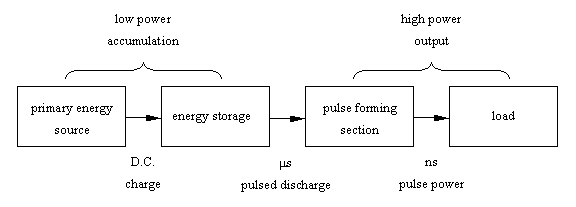
\includegraphics[height=4cm,width=8cm,keepaspectratio=true]{HPMsystem}
 \caption{Primjer ubacivanja slike.}
 \label{fig:prva}
	\end{center}
\end{figure}
\end{verbatim}
Uočite uporabu naredbe \verb|\label| unutar bloka. Na nju se potom u tekstu možemo referencirati pisanjem npr.\ \verb|Na Slici~\ref{fig:prva}| čime \LaTeX{} u tekst uvrsti pripadajući broj slike, kao npr.\ ``Na Slici~\ref{fig:prva} prikazana je osnovna shema HPM sustava.''
Znak \verb|~| iza riječi Slici osigurava točno jedan znak razmaka, što pomaže ukoliko je riječ Slika na kraju retka, da ne razdvoji riječ Slika i pripadajući broj slike.

\begin{figure}[!htbp]
	\begin{center}
 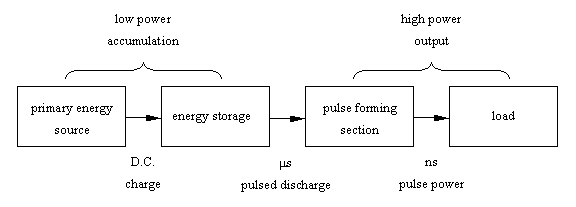
\includegraphics[height=4cm,width=8cm,keepaspectratio=true]{HPMsystem}
 \caption{Primjer ubacivanja slike.}
 \label{fig:prva}
	\end{center}
\end{figure}

Uočite i način prilagođavanja veličine slike. Parametri slike \emph{width} i \emph{height} određuju maksimalne dopuštene dimenzije pri čemu se primarno poštuje manju navedenu dimenziju, a \emph{keepaspectratio} osigurava zadržavanje odnosa dimenzija slike, odnosno sprječava deformaciju slike, nakon proizvoljno unesenih veličina.

Uočite da sve oznake tj.\ \emph{labeli} ne smiju imati razmak u imenu. To vrijedi i općenito, a ne samo za slike.

Također, uočite da nije potrebno pisati ekstenziju slike jer to je uređeno u postavkama glavnoga dokumenta pa time štedi trud. Ekstenzije koje se može izostaviti su: \emph{jpg}, \emph{jpeg}, \emph{png} i \emph{pdf}.

Shema prikazana na Slici~\ref{fig:prva} će biti korištena i za potrebe idućih primjera, a {\color{blue} u mapi na vašem disku ju obrišite nakon što počnete pohranjivati vlastite slike vezane uz vaš rad}.


\section{Ubacivanje podslika}
Ponekada se jedna slika sastoji od dvije ili više podslika kojima želimo opisati neku cjelinu. Slika će dobiti pripadni broj, a podslike slova (a), (b) itd.
To se može postići sljedećom strukturom:
\begin{verbatim}
\begin{figure}[!htpb]
 \begin{center}
  \subfloat[Blok shema HPM sustava.]{\label{fig:HPM}
   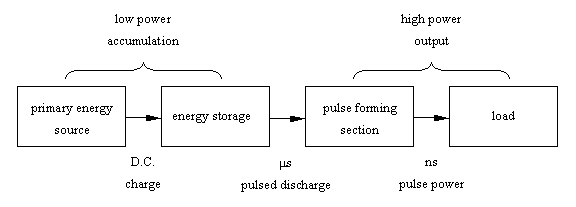
\includegraphics[height=5cm,width=10cm,keepaspectratio=true]{HPMsystem}}\\ 
	    %\hspace{10pt}
   \subfloat[JabRef sučelje za unos ``elektroničke'' reference.]
   {\label{fig:jabref}
   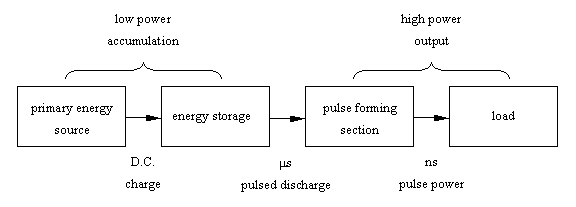
\includegraphics[height=7cm,keepaspectratio=true]{HPMsystem}}
\caption{Primjer ubacivanja više podslika. Ovo je opis cijele slike.}
\label{fig:dvije_podslike}
  \end{center}
\end{figure}
\end{verbatim}
što će uvrstiti ono što se vidi na Slici~\ref{fig:dvije_podslike}, koja se sastoji od dviju podslika.
Podslika~\ref{fig:HPM} pokazuje shemu HPM sustava, a podslika~\ref{fig:jabref} sučelje JabRef programa za unos bibliografskih jedinica.

\begin{figure}[!htpb]
	  \begin{center}
	   \subfloat[Blok shema HPM sustava.]{\label{fig:HPM} 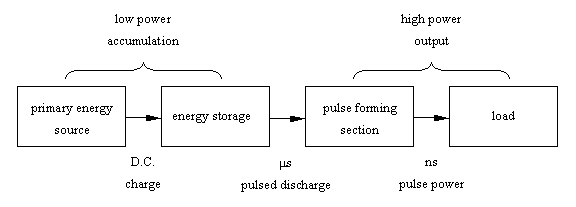
\includegraphics[height=5cm,width=10cm,keepaspectratio=true]{HPMsystem}} \\ %\hspace{10pt}
	   \subfloat[JabRef sučelje za unos ``elektroničke'' reference.]{\label{fig:jabref} 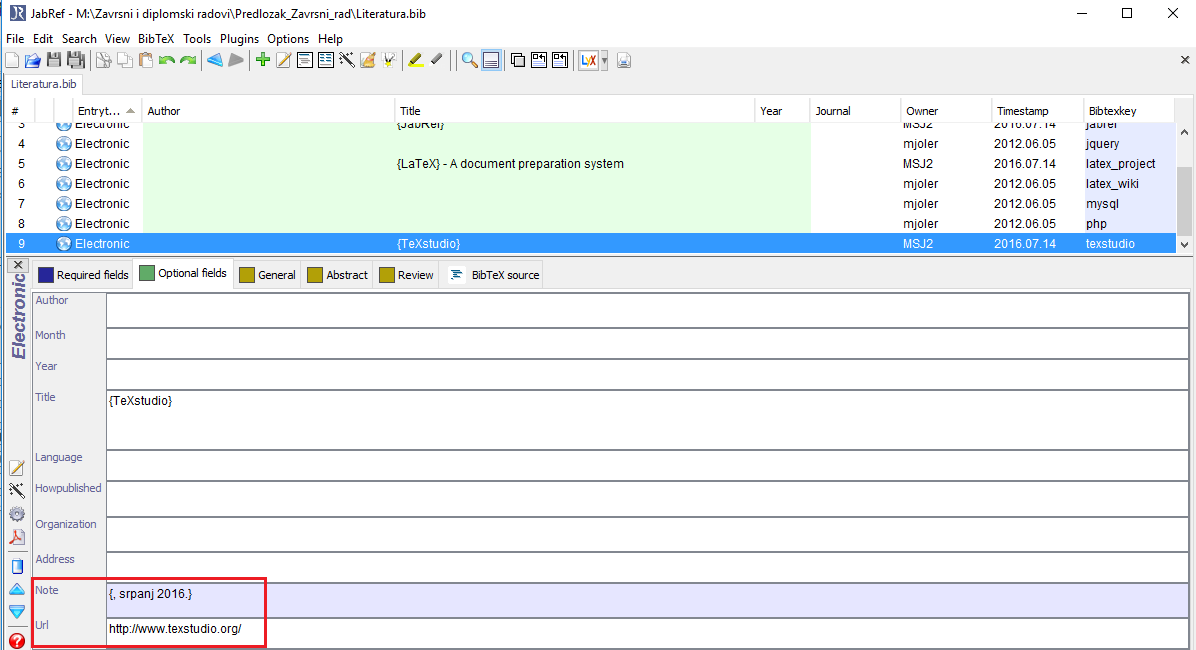
\includegraphics[height=7cm,keepaspectratio=true]{jabref}}
\caption{Primjer ubacivanja više podslika. Ovo je opis cijele slike.}
\label{fig:dvije_podslike}
	  \end{center}
\end{figure}



\section{Ubacivanje tabele} 
Više detalja o kreiranju tabela pročitajte u literaturi, a sljedeći blok vam omogućava kreiranje jednostavne tabele, kao što je prikazano u Tabeli~\ref{tab:prva}.
\begin{verbatim}
\begin{table}[!htbp]
\renewcommand{\arraystretch}{1.2}
\caption{Ovo je primjer izrade tabele.}
\centering
\begin{tabular}{|c|c|c|}
\hline
variabla & vrijednost 1 & vrijednost 2  \\ [0.5ex]
\hline \hline  
A & 5 & 3 \\ [0.5ex] % razmak do iducega retka
B & 4 & 2 \\ [0.5ex]
\hline
\end{tabular}
\label{tab:prva}
\end{table}
\end{verbatim}

\begin{table}[!htbp]
\renewcommand{\arraystretch}{1.2}
\caption{Ovo je primjer izrade tabele.}
\centering
\begin{tabular}{|c|c|c|}
\hline
variabla & vrijednost 1 & vrijednost 2  \\ [0.5ex]
\hline \hline 
A & 5 & 3 \\ [0.5ex] % razmak do iducega retka
B & 4 & 2 \\ [0.5ex]
\hline
\end{tabular}
\label{tab:prva}
\end{table}
%
Podaci koji su u stupcima se u tabeli razdvajaju znakom \&. Novi redak se na kraju aktualnoga retka formira znakom \verb|\\|. Broj stupaca se definira iza \emph{tabular} time što se navedu slova koja označavaju poravnavanje teksta u svakom stupcu, a broj slova znači broj stupaca koji će biti kreiran u tabeli. Vertikalni razmak između redaka u tabeli možete za cijelu tabelu prilagoditi uporabom sljedeće sintakse prije strukture za tabelu:\\
\verb| \renewcommand{\arraystretch}{1.2} | gdje broj u zagradi na kraju (ovdje je 1.2) prilagodite sukladno vašoj preferenciji. Može se prilagoditi i razmak za svaki pojedini redak (uočite \verb|[0.5ex]| na kraju redaka), ali to je manje od interesa jer tipično želimo da svi retci imaju jednaki razmak jedni od drugih.

Slično možete učiniti i za razmak između stupaca tabele navođenjem sljedeće sintakse prije bloka tabele:\\
\verb| \renewcommand{\tabcolsep}{0.3cm} |.



\section{Uporaba kratica u tekstu. Automatsko generiranje popisa kratica.}  \label{sec:kratice}
Listu kratica definirajte u datoteci \verb|Kratice.tex| (vidjeti predložak unutar datoteke). U redovitom tekstu, kraticu  možete ubaciti korištenjem naredbe \verb|\gls{ID_kratice}| gdje je \verb|ID_kraticE| identifikator kratice kako je definiran u datoteci \emph{Kratice.tex}. Pri prvoj uporabi naredbe \verb|\gls|, ispisat će se najprije puni naziv pojma pa u zagradi kratica, a kod svake sljedeće uporabe, ispisat će se samo kratica. Na primjer, kada (nakon prethodnog deklariranja u datoteci \verb|Kratice.tex|) upotrijebite \verb|\gls{gsm}| prvi puta, u tekstu će se ispisati \gls{gsm}, a kada upotrijebite \verb|\gls{gsm}| drugi puta i dalje, u tekstu će se ispisati samo \gls{gsm} (usporedi s definicijom kratice u datoteci \verb|Kratice.tex|). 
 
{\color{red} Listu kratica generirate sljedećim postupkom:} \label{generiranje_liste_kratica}
\begin{enumerate}
	\item Pokrenite kompilaciju cijeloga teksta jedanputa (to će generirati neke datoteke koje su potrebne za daljnju obradu, specifično one s ekstenzijama .ist i .glo).
	\item Otvorite \emph{Command Prompt} aplikaciju na vašem računalu i postavite se u radnu mapu gdje su vam datoteke za diplomski rad. 
	\item Potom pokrenite \emph{makeindex} rutinu (ona će tipično biti već prisutna na vašem računalu) upisujući sljedeću sintaksu: \\
	\verb|makeindex   -s myDoc.ist  -o myDoc.gls   myDoc.glo| \\
	gdje naziv datoteke \emph{myDoc} treba zamijeniti nazivom vaše glavne .tex datoteke, (npr. \verb|JMBAG_Ime_Prezime.tex|).
	\item Pokrenite \LaTeX{} još jednom ili dva puta, ako treba, dok se u uvodu pdf dokumenta ne pojavi lista kratica (pod naslovom \emph{Pojmovnik}).	
\end{enumerate}

Možda isprva zvuči složeno, ali zapravo nije (bar ne uz ovako precizne upute!). Svaki puta kada dodate nove definicije kratica, potrebno je ponoviti ovaj postupak da bi se ažurirale odgovarajuće datoteke i uredno prikazala potpuna lista u pdf-u (a i izbjegle poruke o pogreškama tijekom kompajliranja teksta). 

Nije teško nakon što prvi puta prođete ovaj postupak i omogućava vam u tekstu biti dosljedan u uporabi određene kratice. Da izbjegnete čuđenje, važno je još reći da će se ovim postupkom automatski stvoriti tek lista kratica koje ste u tekstu upotrijebili uporabom sintakse \verb|\gls|, a ne na temelju liste definicija koje ste naveli u datoteci \verb|Kratice.tex|. Zato, ako nijednom u tekstu ne upotrijebite sintaksu \verb|\gls|, neće biti ispisan ni popis kratica tj.\ \emph{Pojmovnik}. {\color{blue} Kako \LaTeX{} na kraju uvijek nagradi trud koji je uložen u savladavanje njegove sintakse, pogodnost ovakvoga automatskoga kreiranja Pojmovnika je i to što uz svaki kraticu \LaTeX{} automatski ispiše i brojeve stranica na kojima se dotična kratica pojavljuje!} U elektroničkom pdf dokumentu, brojevi stranica su ujedno i hiper-veze na te stranice pa se tako može odmah skočiti na stranicu gdje je pojedina kratica upotrijebljena.

Ukoliko vam se prethodno opisani postupak čini presloženim, popis kratica možete napraviti i ručno, isto pomoću datoteke Kratice.tex, u kojoj također postoji kratki predložak i za takav pristup. Za to je onda u osnovnoj datoteci \verb|JMBAG_Ima_Prezime.tex| potrebno deaktivirati liniju koda koja počinje sa \verb|\printglossary|, a aktivirati blok koji počinje sa \verb|\begin{glossary}| i završava sa \verb|end{glossary}|.



\section{Naglašavanje teksta}
\subsection{Navodnici}
Za navodnike s lijeve strane fraze (otvaranje navodnika) koristi se 2x jednostruki navodnik koji se na tipkovnici nalazi lijevo od broja 1, a za navodnike s desne strane fraze (zatvaranje navodnika), koristi se 2x jednostruki navodnik koji se na tipkovnici nalazi na tipki \emph{ć}, što proizvede npr.\ ``abc''.

{\color{blue} Alternativno, u ovom paketu je pripremljena i naredba {\color{red} \verb|\navod{abc}|} gdje je \emph{abc} tekst koji se stavlja između navodnika, tj.\ \navod{abc}.}

\subsection{Kosa i podebljana slova}
Naglašavanje neke riječi ili fraze pomoću kosih (italic) slova možemo dobiti uporabom naredbe {\color{red} \verb|\emph{abc}|} ili pomoću  {\color{red}\verb|\textit{abc}|} gdje je \emph{abc} neki tekst koji se želi naglasiti.

\textbf{Podebljana slova} možemo postići uporabom naredbe {\color{red} \verb|\textbf{abc}|} gdje je \textit{abc} neki tekst koji želimo podebljati.

\section{Verbatim: okruženje za doslovni tekst}
Verbatim okruženje omogućava ispis teksta u izvornom obliku, bez da ga \LaTeX{} tumači po svojiim sintaktičkim pravilima. To je pogodno kada se na stranicu  npr.\ želi kopirati dio programskoga koda iz nekog jezika i kada želimo zadržati sve izvorne znakove u nekoj frazi, bez da \LaTeX{} počne javljati pogreške kod kompajliranja, što bi se moglo pojaviti kada se ne bi koristilo \emph{verbatim okruženje}, pošto bi neke znakove interpretirao kao pogreške u sintaksi.

Postoji kraći i duži oblik verbatima. Kraći služi za kraću frazu od jedne ili par riječi, a duži za više redaka.

\noindent Kraći oblik verbatima ima sintaksu: \verb+\verb|neka fraza|+

\noindent Duži oblik verbatima ima sintaksu:\\
\verb|\begin{verbatim}| \\
\verb|neki tekst| \\
\verb|\end{verbatim}| \\


\section{Kreiranje jedne jednadžbe ili serije jednadžba}

\subsection{Kreiranje jedne jednadžbe}
Jednadžba se napiše u posebnom matematičkom modu koji se kreira pomoću bloka:
\begin{verbatim}
	\begin{equation}
		 A = B + C   \label{eq:prva}
	\end{equation}
\end{verbatim}
što će dati sljedeći izgled:
\begin{equation}
	 A = B + C   \label{eq:prva}
\end{equation}
Da bi se na nju referenciralo, na željenom mjestu u tekstu upišemo \verb|\eqref{eq:prva}|, čime će se uvrstiti njezin pripadni (automatski generirani) broj, a za potpuniji smisao možemo npr.\ napisati \verb| Jednadžba~\eqref{eq:prva}|, rezultat čega je da će u tekstu pisati Jednadžba~\eqref{eq:prva}. 
Ako ju se ne želi numerirati, onda se nakon riječi \emph{begin} stavi zvjezdica, tj.\ \verb|begin*{equation}|.

\subsection{Kreiranje grupe jednadžba}
Grupa jednadžba se kreira uporabom \emph{subequations} sintakse. Na primjer, sljedeći blok će definirati dvije podjednadžbe u grupi, gdje će svaka biti numerirana istim brojem, a razlikovati slovom iza broja.
\begin{verbatim}
	\begin{subequations}
		\begin{align}
		        A &= B + C  	\label{subeq:prva} \\
		        D &= F + G		\label{subeq:druga}
		\end{align}
	\label{subeq:obje}
	\end{subequations}
\end{verbatim}

To će u izlaznom dokumentu rezultirati sljedećim izgledom:
\begin{subequations}
\begin{align}
        A &= B + C  	\label{subeq:prva} \\
        D &= F + G		\label{subeq:druga}
\end{align}
\label{subeq:obje}
\end{subequations}
U \eqref{subeq:prva} je prikazano dobivanje vrijednosti $A$, a u \eqref{subeq:druga} je prikazano dobivanje vrijednosti $D$. Jednadžba~\eqref{subeq:obje} je \emph{čuveni studentov zakon}!



\section{Liste}
Liste su česte forme u tekstu kojima se na pregledni način nabrajaju neke stavke. Stavke obično navodimo ili s točkama na početku, s brojevima ili sa slovima. U \LaTeX-u su upravo ta tri stila unaprijed definirana, a moguće su i složenije definicije stilova i kombinacije lista.

\subsection{Lista s točkama}
Lista s točkama se postigne blokom
\begin{verbatim}
\begin{itemize}
    \item prva nenumerirana stavka
    \item druga nenumerirana stavka
\end{itemize}
\end{verbatim}
što na ekranu proizvede:
\begin{itemize}
% \setlength\itemsep{1ex}   % za lokalnu prilagodbu
	\item prva nenumerirana stavka
	\item druga nenumerirana stavka
\end{itemize}

\subsection{Lista s brojevima}
Numerirana lista s brojevima se postigne blokom
\begin{verbatim}
\begin{enumerate}[itemsep=1ex, topsep=4pt, partopsep=0pt]
     \item prva numerirana stavka
     \item druga numerirana stavka
\end{enumerate}
\end{verbatim}
U uglatoj zagradi su tri parametra kojima se točno može kontrolirati vertikalni razmak između stavki u listi (\emph{itemsep}), razmak između prethodnoga teksta i prve stavke u listi (\emph{topsep}) i dodatni prostor između liste i prethodnoga paragrafa kada lista započinje novi paragraf (\emph{partopsep}), ali te parametre \textbf{ne morate navoditi} tj.\ tu uglatu zagradu ne morate pisati. Tada će se primijeniti vrijednosti parametara koje su definirane za cijeli dokument, a ove parametre se može upotrijebiti tek da u nekom pojedinom slučaju prilagodite razmake.
Za osjetiti efekte ovih parametara, najbolje se malo sam poigrati različitim vrijednostima parametara i vidjeti posljedice toga na listu (pri tome se uz brojeve kao prikladne jedinice za razmak mogu koristiti \emph{pt}, \emph{ex} ili \emph{em}).

\subsection{Proizvoljno označena lista}
Takva se lista može postići u sklopu općenitije forme koja omogućuje proizvoljni opis ispred pojedine stavke, pomoću sljedećega bloka:
\begin{verbatim}
\begin{description}
     \item[a)] prva opisna stavka
     \item[b)] druga opisna stavka
\end{description}
\end{verbatim}
što na ekranu proizvede:
\begin{description}%[itemsep=1ex, topsep=4pt, partopsep=0pt] za lokalnu prilagodbu
	\item[a)] prva opisna stavka
	\item[b)] druga opisna stavka \\
\end{description}
%
Kod ove strukture, u uglatu zagradu iza naredbe \verb|\item|, navodi se proizvoljna oznaka kojom se želi na neki način ``numerirati'' listu.
%:::::::::::::::::::::::::::::::::::::::::::::::::::
\chapter{Dodatne informacije}
\section{Primjeri uporabe sintaktičkih struktura}
\begin{enumerate}
	\item Za uvid u kontekstualnu primjenu raznih sintaktičkih struktura, možete otvoriti datoteku \href{run:Intro.tex}{{\color{blue}Intro.tex}}, unutar koje su napisane i ove upute. 
	\item Primjere složenijih sintaktičkih struktura, kao što su ubacivanje slike, tabele ili jednadžbe, možete naći u datoteci \href{run:sintaksa_cestih_struktura.tex}{{\color{blue}sintaksa\_cestih\_struktura.tex}} koja je dio paketa. Odabrane se strukture može kopirati i zalijepiti u vaš tekst, uz minimalne prilagodbe kao što su naziv slike, veličina slike, opis i ID slike, a analogno i za tabele i jednadžbe.
	\item Konačno, za više detalja o bilo čemu, potražite informacije u dvama priručnicima koji su priloženi u mapi \href{run:prirucnici}{{\color{blue}prirucnici}} ili na webu, gdje se, među obiljem drugih informacija, nalaze i korisne wiki stranice \cite{latex_wiki,tex_exchange} o \LaTeX-u pomoću kojih se obično brzo pronađe upute i zadovoljavajuće rješenje kakvom sintaksom se može urediti željeni dio teksta.
\end{enumerate}

\section{Savjeti za lakše uređivanje teksta}
Vjerujem da vam ovaj dokument može uvelike pomoći u pripremi teksta vašega završnog/diplomskog rada i omogućiti da glavninu vremena trošite na sadržaj rada, a manje na formatiranje rada jer to će za vas sada obaviti \LaTeX{}! 

No, korektnosti radi, potrebno je napomenuti i sljedeće: \LaTeX{} je vrlo osjetljiv na pogreške u sintaksi naredbi (da, baš kao što su i programski jezici) pa vas može povremeno ugnjaviti javljanjem pogreške koju nikako ne uspijevate uočiti gdje je. Iskustvo kojim se izbjegava ta nelagoda jest sljedeće:
\begin{itemize}
	\item svako poglavlje napišite u novoj datoteci (da biste količinu teksta razdvojili na preglednije i manje cjeline) koju imenujte prikladnim imenom (bez razmaka u imenu). Potom te datoteke samo pozivajte iz glavnoga dokumenta \verb|JMBAG_Ime_Prezime.tex| pomoću naredbe \verb|\include{ime_datoteke}|. Takav je pristup upravo i korišten u pripremi ovoga paketa.
	%
	\item {\color{red} budite koncentrirani dok pišete \LaTeX{} naredbe, poglavito zagrade, posebne znakove i matematički tekst gdje se zahtijeva uporaba znaka \$!}
	%
	\item kompajlirajte tekst prije nego se skupi puno teksta jer tako ćete imati manje teksta za prekontrolirati u slučaju pogreške. Također vam za provjeru tek manjega dijela dokumenta može pomoći paket \verb|\usepackage{syntonly}| i naredba \verb|syntaxonly|, a isto tako i naredba \verb|\includeonly{ime_datoteke}| kojom ćete kompajlirati samo tu navedenu datoteku, čime  ispred ``neželjenih'' datoteka ne morate stavljati znak ``komentara'' (\%).
	%
	\item ako niste sigurni hoće li vam raditi neka naredba nakon pisanja, radije tekst kompajlirajte odmah po pisanju te naredbe---da vidite što ćete dobiti i riješite dvojbu, nego da čekate da se skupi još dubioznih mjesta u tekstu, kada će nakon kompajliranja biti teže detektirati koja linija teksta zapravo izaziva probleme (\LaTeX-ov prozor s porukama često nije odveć precizan u lociranju i opisu pogrešaka, ovisno o editoru teksta koji koristite).
\end{itemize}


\section{Završne napomene}
Ovime zaključujemo uvodne upute koje će najvećem broju studenata biti dovoljne (ili barem dovoljna osnova) za uspješno pisanje završnog odnosno diplomskog rada.

Prije nego prijeđete na kreiranje vlastitoga sadržaja učinite još sljedeće akcije kojima ćete deaktivirati dio paketa koji će biti nepotreban:
\begin{enumerate}
	\item u mapi \href{run:slike}{{\color{blue}slike}}, obrišite datoteke \verb|HPMsystem.png| i \verb|jabref.png| jer su one služile tek za ilustracije u ovim Uputama.
	%
	\item u glavnoj datoteci  \href{run:JMBAG\_Ime\_Prezime.tex}{{\color{blue}JMBAG\_Ime\_Prezime.tex}} stavite znak komentara ``\%'' ispred linije \verb|
\chapter{Kako koristiti paket za pisanje završnoga rada u \LaTeX-u}
Ovo su uvodne napomene za korištenje predloška za pisanje završnoga ili diplomskoga rada studenata Tehničkoga fakulteta u Rijeci. Prije korištenja paketa, pročitajte ovaj tekst jer će vam dati nužne uvodne informacije, znatno vam olakšati i ubrzati uređivanje teksta nakon toga, pri čemu će vas i voditi kroz uporabu ovoga paketa na praktičan način.

Paket je pripremljen tako da student što prije može pisati vlastiti tekst u već pripremljenom predlošku koji će, uz minimalno učenje sintakse \LaTeX-a, studentu olakšati urediti svoj rad. U paketu su uključene potrebne upute i sintaktičke strukture koje bi trebale udovoljiti potrebama većine studenta, a dodatne informacije postoje u dvama priručnicima koji su uključeni u ovom paketu te, naravno, na raznim web stranicama na internetu koje su posvećene \LaTeX-u (vidi u nastavku).

{\color{red} POZOR: paket treba biti prekopiran negdje na disk ne mijenjajući originalnu strukturu mapa (foldera) i ne mijenjajući nazive datoteka koje su u mapi \emph{tex\_aux}!}


\section{Opis sadržaja paketa}
\vspace{-2ex}
Paket se sastoji od:
\begin{itemize}
 \item datoteke \href{run:UPUTE.pdf}{{\color{blue} UPUTE.pdf}} koja sadrži postupak instalacije potrebnih alata na računalo te korištenja paketa. \emph{UPUTE} su bazirane na Windows OS, a korisnici drugih OS-ova si na naznačenim web lokacijama samo trebaju naći instalacije za njihov OS.
 %
 \item datoteke \verb|JMBAG_Ime_Prezime.tex| koja je središnja datoteka koja povezuje sve cjeline i kompajliranjem koje se dobije izlazni \verb|JMBAG_Ime_Prezime.pdf| dokument (naravno, tijekom rada, upisat ćete svoj specifični JMBAG i ime i prezime).\\ U ovoj se datoteci inicijalno nalaze i upute za korištenje paketa kao i primjeri osnovne uporabe najčešćih sintaktičkih struktura u \LaTeX-u koje bi trebale biti dovoljne većini studenata za pisanje rada.
 %
 \item mape \verb|tex_aux| u kojoj su \emph{interne datoteke} koje definiraju stilove, formate i sl.\ koji služe u slaganju izlaznoga formata. \textbf{Student/ica s njima ne treba \emph{ništa} raditi}, ali one trebaju biti u \verb|tex_aux| mapi pod glavnom mapom završnoga rada, kao što je postavljeno u ovom paketu.
 %
 \item mape \emph{slike} u koju student treba pohraniti sve slike koje će koristiti u radu. Ime mape se ne smije preimenovati bez boljega poznavanja sintakse \LaTeX-a jer ovaj paket da bi ispravno radio očekuje baš takvo ime mape!
 %
 \item datoteke \verb|sintaksa_cestih_struktura.tex| koja ne sudjeluje izravno u kompajliranju pdf dokumenta, nego služi kao repozitorij u kojemu su sadržane najčešće potrebne sintaktičke strukture koje su spremne za kopiranje u vaš tekst uz minimalnu prilagodbu parametara (npr.\ opis slike, ime datoteke specifične slike koju se ubacuje i proizvoljni ID te slike za kasnije referenciranje).
 %
 \item mape \href{run:prirucnici}{{\color{blue}prirucnici}} u kojoj se nalazi nekoliko najpopularnijih priručnika za uporabu \LaTeX-a. 
\end{itemize}
%%%%%%%%%%%%%%%%%%%%%%%%%%%%%%%%%%%%%%%%%%%%%%%%%%%%%%%%%%%%%%%
\section{Čime se opremiti za pisanje rada}
Da bi se rad napisao pomoću \LaTeX-a (a to vrijedi svake lipe!), najprije je na računalo potrebno instalirati:
\begin{enumerate}
	\item obavezno: \LaTeX{} software 
	\item obavezno: editor za uređivanje teksta 
	\item neobavezno, ali korisno: softver za opis literature. (Premda dodatni softver nije nužan jer se popis literature može obraditi i ručno (no to je manje sofisticirano kod uvrštavanja referenca), sugeriram instalaciju softvera koji pomoću intuitivnih sučelja korisniku omogućava opis pojedine korištene literature (kao mala baza podataka), a potom se pojedina jedinica literature jednostavno ubacuje u tekst, a popis literature se na kraju automatski formira (više o tome pročitajte u nastavku).
\end{enumerate}

\subsection{Instalacija \LaTeX-a}
\begin{enumerate}
	\item odite na središnji \LaTeX{} portal \cite{latex_project}: \url{http://www.latex-project.org/}
	\item kliknite na poveznicu \href{http://www.latex-project.org/ftp.html}{Getting LaTeX} i potom uočite i povucite instalaciju koja odgovara vašem OS-u (npr.\ proTeXt za Windows, MacTeX za Mac, TeX Live za Linux). Pozor: instalacijski paket je velik i može duže potrajati čak i na brzoj vezi---dajte si dovoljno vremena za obaviti download.
	\item Instalirajte \LaTeX{} slijedeći upute koje su priložene za odabranu instalaciju (npr.\ proTeXt za Windowse daje kratki pdf s uputama koje vas vode kroz instalaciju korak po korak).
\end{enumerate}

\subsection{Instalacija editora teksta}
Instalirajte editor koji je pogodan za pisanje \LaTeX{} koda. \textbf{Za Windows OS, toplo preporučam}  \href{http://www.texstudio.org}{{\color{blue} TeXstudio}} \cite{texstudio} jer je bogat opcijama, ugodan za rad i stabilan, a instalacije postoje i za Linux i Mac OS. TeXstudio se zasebno povuče i instalira na računalo, a neke editore teksta koji već dođu u paketu za instalaciju LaTeXa možete ignorirati (npr.\ za Windows je do nedavno bio popularan \emph{TeXnicCenter} i dolazi već upakiran u proTeXt-u (a možda ćete naći i \emph{TeXworks}), za Mac je kvalitetan \emph{TeXShop} koji sada također dolazi u paketu s MacTeX-om). 

\label{encoding1} {\color{red} POZOR: Premda će ovo biti još napomenuto na stranici~\pageref{encoding2}, prije samoga početka pisanja vašega rada, što prije želim napomenuti sljedeći važni detalj: za svaki vaš tekst koji pišete u editoru teksta, uvjerite se da je kodna stranica postavljena na \navod{windows-1250}, što je ključno da bi se u izlaznom pdf-u ispravno ispisivali hrvatski dijakritički znakovi! U TeXstudiu, aktualnu kodnu stranicu se može vidjeti i promijeniti preko maloga izbornika u doljnjem desnom kutu glavnoga prozora, gdje se nalazi opcija ``Encoding''. Ukoliko tu ne piše ``windows-1250'', kliknite na izbornik, odaberite opciju ``More Encodings'' pa u potom otvorenom sučelju odaberite kodnu stranicu ``windows-1250 / CP 1250'' i potvrdu sa ``Change To''.}

\subsection{Instalacija programa za opis korištene literature}
\emph{Ponavljamo: Korištenje BiBTeX programa za opis literature \textbf{nije} neophodno, ali jest korisno. U datoteci po imenu \href{run:Literatura.tex}{{\color{blue}Literatura.tex}}, koja je uključena u ovaj paket, već su namještene postavke kao da će se literatura opisati pomoću BiBTeX programa (npr.\ JabRef-a) i ne treba ništa mijenjati, ali ispod toga se može pronaći i upute i za drugi--ručni-- način (p)opisivanja literature.}

Kao bibtex program za opis literature, preporučam \href{http://www.jabref.org}{{\color{blue} JabRef}} program \cite{jabref}. To je legalno besplatno dostupni program za Windows OS (ali postoji i za Mac, a i platformski neovisna instalacija) koji nam omogućava opisivanje literature na lak način pomoću intuitivnih sučelja, a kao rezultat kreira \emph{BibTeX} datoteku \emph{Literatura.bib} (gdje je (\emph{Literatura} naziv koji korisnik treba dodijeliti pri pohrani JabRef datoteke na disk u slučaju ovoga predloška, da bi paket funkcionirao) u kojoj je literatura opisana na način koji \LaTeX{} razumije. 

Uočite da ako ne koristite JabRef, već se odlučite za ručni unos literature, što se isprva doima jednostavnijim, tada će vam redoslijed referenca u popisu literature odgovarati točno redoslijedu koji ste naveli u tom popisu --- dakle morate paziti da redoslijed formirate onim redom kojim pozivate reference u vašem tekstu (što kod nekog kasnije ubacivanja dodatne reference unutar već postojećega redoslijeda traži brigu da ju se ubaci na odgovarajuće mjesto u popisu literature), a također trebate paziti i na formatiranje teksta svake reference! 

Za razliku od toga, korištenjem JabRef-a, izbjegavate ručno formiranje popisa literature i ne trebate brinuti o redoslijedu referenca, već samo pomoću JabRefa trebate unijeti sve jedinice literature koju ćete navesti, a \LaTeX{} će vam automatski formirati listu referenca onim redoslijedom kojim reference bude pozivali u tekstu!

Nakon što kompajlirate projekt, stvorit će vam se pomoćna datoteka imena \href{run:JMBAG_Ime_Prezime.bbl}{{\color{blue}JMBAG\_Ime\_Prezime.bbl}} u kojoj će jedinice literature tijekom kompilacije biti formatirane i odatle se ubacuju u konačnu verziju teksta. Stoga, \textbf{ukoliko ima ikakvih detalja koje u opisu literature treba prilagoditi, a ne možete automatskim putem}, uvijek vam kao ``zadnja crta obrane'' ostaje otvoriti \verb|bbl| datoteku i tamo ručno napraviti izmjene. Potom ponovo kompajlirajte projekt i te će se promjene vidjeti u pdf-u tj.\ ručno unijete promjene neće biti poništene sve dok ne obrišete cijelu datoteku.

Umjesto da rukom pišete cijelu bibliografiju, vremenski vam je vjerojatno učinko\-vitije popis literature generirate uporabom JabRef-a, a potom ako išta još treba prilagoditi, onda samo to napraviti ručno u \verb|bbl| datoteci.


\subsubsection{Osnovna uporaba JabRef programa}
Upoznajte se s najvažnijim opcijama u \emph{JabRef}-u:
\begin{itemize}
	\item uočite ikonu (pod znakom ``+'' i tekstom \emph{New BibTeX Entry}) za unos nove jedinice literature (npr. knjige, članka, web portala i sl.)
	%
	\item kada kliknete za unos nove stavke literature, uočite kakvi se sve tipovi literature nude za odabir. Odabirom opcije koja odgovara naslovu koji želite unijeti, otvorit će vam se novi prozor s poljima u koja se može unijeti informacije o literaturi. Za odabrani tip literature samo su neka polja obavezna (nalaze se pod karticom (eng.\ \emph{tabom}) \emph{Required fields}), dok se pod drugim karticama može i ne mora unijeti dodatne informacije. U slučaju naših završnih/diplomskih radova, bit će znatan udjeli literature koja je na internetu pa za formatiranje iste, pročitajte upute i napomene u nastavku ove sekcije.
	%
	\item kada je više autora, njihova imena se u JabRefu polju za unos autora razdvajaju pisanjem ključne riječi \verb|and| (a ne razmakom, zarezom ili točka-zarezom!)
	%
	\item U popisu literature se neće uvijek pojam prepisati onako kako ste ga vi zapisali u JabRefu! To je posljedica stilova koji su definirani u \verb|bst| datoteci (ne zamarajte se time sada jer je za naprednu razinu \LaTeX-a). No, ako neki pojam baš ne ispadne suvislo napisan u popisu literature ili baš želite forsirati određeni način zapisa (često slučaj kada se riječ s velikim slovima ne interpretira onako kako želite), tada točno određeni zapis možete forsirati na način da \verb|{tu riječ ili frazu stavite unutar vitičastih zagrada}|
	%
	\item prije nego pohranite pojedinu stavku pomoću \emph{Ctrl+S}, \textbf{morate svakoj jedinici literature dodijeliti jedinstveni identifikator}, tzv.\ \emph{Bibtexkey}, što je jedno od polja koja su obavezna za unos. Možete ručno upisati neki proizvoljni string, ali pogodnije je generirati ga automatski.\\ Za to učiniti među ikonama na vrhu imate ikonu koja izgleda kao (čarobni) štapić sa zvjezdicama oko njega, klikom na kojega \emph{JabRef} automatski dodijeli jedinstveni BibTeX \emph{ključ} za tu bibliografsku jedinicu. Pomoću toga ključa se poslije bilo kada i bilo gdje u pisanju vašega rada možete pozvati na tu referencu, a \LaTeX{} će sve ostalo obaviti za vas tj.\ dodijeliti joj odgovarajući broj u tekstu i s tim brojem uvrstiti u popis literature.
	%
	\item korisnik ima mogućnost i promijeniti uzorak po kojem se kreira struktura automatski generiranoga jedinstvenoga BibTeX ključa tako da se otvori opcija izbornika \emph{Options $>>$ Preferences $>>$ BibTeX key generator}, gdje je na vrhu prozora prikazan \emph{default} uzorak, npr. \verb|[auth]:[year]| što znači da se ključ kreira na bazi \verb|prezime(autora):godina(rada)|. To se sada može urediti po nekom novom uzorku, no ovako definirani uzorak u biti zadovoljava, a ako igdje ima potrebe za dodatnim razlikovanjem, može se na automatski generiranom ključu još ručno napraviti korekcija dodavanjem nekog znaka na kraju, kao npr.\ dodavanjem \verb|_a| i sl. (Klikom na karticu \emph{BibTeX source} možete vidjeti kako će unos vaših podataka zapravo biti zapisan u vašoj \emph{Literatura.bib} datoteci koja će se formirati od svih bibliografskih jedinica koje unesete.)
	%
	%
	\item Za \emph{ime} vaše bibliografske datoteke kod pohrane na disk obavezno upišite  \emph{Literatura} jer to ime očekuje ovaj paket. Pozor: Datoteka \emph{Literatura.bib}, koju ste tako kreirali, mora se nalaziti unutar mape ovoga paketa da bi sve ispravno radilo! U paketu je za primjer već kreirana jedna datoteka istoga imena koju za vježbu student može i otvoriti u \emph{JabRef}-u, ali to su samo pokazne bibliografske jedinice unesene kao primjer, koje student treba u konačnici zamijeniti svojim bibliografskim jedinicama.
	%
	\item Za ``elektroničke'' izvore literature (tj.\ sve što ste kao informaciju našli na webu), JabRef nudi tip literature pod nazivom ``Electronic'' (vidi Sl.~\ref{fig:jabref}). U njemu pod karticom (eng.\ tabom) \emph{Optional fields} pod poljem \verb|Title| možete upisati ime web stranice (autor, tvrtka i sl.), pod poljem \verb|url| možete upisati URL adresu te web stranice, a pod poljem \verb|Note| upisati datum kada ste posjetili tu web stranicu (npr.\ \emph{srpanj 2016.} ili \emph{3.~rujna~2016.}). Rezultat toga će u pdf-u biti da je sve napisano redoslijedom koji je predviđen u Uputama RiTeha za pisanje diplomskog rada \cite{riteh_upute}, \emph{osim što u ovom Predlošku do sada nisam uspio riješiti ubacivanje zareza između URL adrese i datuma posjeta toj URL adresi}, koji bi ta dva podatka odvojio, pa je tu potrebna mala ručna \emph{prilagodba na jedan od ovih dvaju načina}:
	\begin{enumerate}[label=\textbf{\roman*)}]
		\item kod unosa datuma u polje \verb|Note| (u sučelju JabRef-a), upišite datum na sljedeći način: \verb|{, <datum>}|, gdje je \verb|<datum>| vaš specifični datum, dok će \emph{zarez} iza prve zagrade izvršiti razdvajanje URL adrese i datuma, a \textbf{vitičaste zagrade} osigurati da se to baš tako točno prenese u pdf-dokument (uključujući i da se mjesec napiše malim početnim slovom, što inače ne bi bio slučaj). (Za neke druge tipove referenca kao npr.\ tip \emph{manual}, zarez vam prije datuma neće trebati jer će naziv literature završiti zarezom.) U Jabrefu vam i inače vrijedi da kada želite forsirati da se pojam baš točno u popisu literature zapiše onako kao ste htjeli, onda se pojam stavi unutar vitičastih zagrada \verb|{kao u ovom primjeru}|.
		\item ako u polju \verb|Note| ne upišete datum na prethodno opisani način, onda vam u pdf dokumentu neće biti upisan zarez između URL adrese i datuma koji ste unijeli, a također će i mjesec biti napisan velikim početnim slovom (što nije strašno, ali je manje poželjno). To možete \emph{ručno} prilagoditi tako da otvorite \verb|.bbl| datoteku i pomoću \emph{Find/Replace} operacije sve nazive mjeseca zamijenite na način da počinju malim početnim slovom (što nije teško kada vam je većina datuma u popisu literature navedena u istom mjesecu), ali zareze ćete svakako morati ubacivati ručno u svaku pojedinu stavku literature jer neće biti nekog predloška kojim biste to riješili automatski pomoću \emph{Find/Replace} operacije. Na kraju opet kompajlirajte projekt. S obzirom na navedeno, prvi način je vremenski štedljiviji!
	\end{enumerate}
\end{itemize}

%%%%%%%%%%%%%%%%%%%%%%%%%%%%%%%%%%%%%%%%%%%%%%%%%%%


\chapter{Primjeri najčešćih sintaktičkih struktura}
Prije stvarnoga početka pisanja svoga rada, upoznajte se s osnovnim sintaktičkim strukturama koje će vam trebati tijekom pisanja rada.

U nastavku su opisane najčešće sintaktičke strukture (dio njih možete naći i u datoteci \emph{Intro.tex}), a dodatne složenije strukture su pohranjene u datoteci \href{run:sintaksa_cestih_struktura.tex}{{\color{blue}sintaksa\_cestih\_struktura.tex}} koja je sastavni dio glave mape ovoga paketa. 

\section{Postavljanje naslova poglavlja i sekcija}
\begin{itemize}
	\item \verb|\chapter{Naslov poglavlja}|: za definiranje naslova poglavlja
	\item \verb|\section{Naslov sekcije}|: za definiranje naslova sekcije unutar poglavlja
	\item \verb|\subsection{Naslov podsekcije}|: za definiranje naslova podsekcije
\end{itemize}


\section{Reference na literaturu} \label{sec:RefLit}
Za referencu na pojedini korišteni izvor informacije (tj.\ jedinicu literature), koristimo naredbu \\
\verb|\cite{bibtexkey}|, gdje je \emph{bibtexkey} jedinstveni ključ kojim prethodno označimo tu jedinicu literature. \verb|Bibtexkey| možemo definirati na jedan od sljedećih načina:
\begin{description}
	\item[I)] ako popis literature definiramo izravno u datoteci \href{run:Literatura.tex}{{\color{blue}Literatura.tex}} (opcija (I) u datoteci), onda ispred svake stavke literature treba definirati i jedinstveni \verb|bibtexkey| pomoću naredbe \verb|\bibitem{bibtexkey}| (vidi predložak u datoteci)
	\item[II)] ako literaturu opisujemo pomoću JabRef datoteke \emph{Literatura.bib} (opcija (II) u datoteci), onda se tamo uz svaku stavku definira \verb|bibtexkey| (bude na dnu JabRef obrasca za upis pojedine jedinice literature)
\end{description}
%
Npr.\ ako negdje u tekstu napišemo \verb|\cite{latex_wiki}|, gdje je \verb|latex_wiki| prethodno definirani \emph{bibtexkey}, tada će se u tekstu u uglatoj zagradi pokazati broj  te bibliografske jedinice pod kojim se nalazi u popisu literature (Bibliografiji) na kraju rada (u ovom primjeru, to je broj \cite{latex_wiki}).


\section{Referenca na sekciju, sliku, tabelu ili stranicu} \label{sec:RefText}

Za referenciranje na pojedine dijelove teksta unutar rada, koristimo
{\color{red} \verb|\label{ID}|} i {\color{red} \verb|\ref{ID}|} na način da se \verb|\label{ID}| postavi uz dio teksta koji želimo označiti internom oznakom i poslije ćemo se u tekstu na to referencirati, a \verb|\ref{ID}| upotrijebimo na mjestu s kojega se referenciramo na dio teksta koji je ranije označen pomoću \verb|\label{ID}|.

Ako se želimo referencirati na specifičnu sliku ili tabelu ili sekciju ili jednadžbu u tekstu, tada unutar bloka toga sadržaja stavimo oznaku \verb|\label{prefiks:ID_objekta}| gdje je \emph{objekt} slika ili tablica ili sekcija teksta ili jednadžba, a na željenom mjestu u tekstu se na to referiramo pomoću \verb|\ref{prefiks:ID_objekta}| (u slučaju referenciranja jednadžbe, bolji oblik naredbe je {\color{red} \verb|\eqref{prefiks:ID_objekta}|}).

\verb|ID_objekta| je proizvoljni string (bez razmaka) koji dodijelimo objektu od interesa, a radi preglednijega uređivanja teksta, uobičajeno je u \LaTeX-u za pojedine tipove oznaka staviti i odgovarajući \emph{prefiks}, kao npr.\ \emph{sec} za oznaku sekcije, \emph{fig} za oznaku slike, \emph{tab} za oznaku tabele, \emph{eq} za oznaku jednadžbe i sl. (Tako bi za sliku kojoj dodijelimo $ID=prva$ bilo \verb|\label{fig:prva}|, za tablicu \verb|\label{tab:prva}|, za sekciju \verb|\label{sec:prva}|, a za jednadžbu \verb|\label{eq:prva}|.)

Za referencirati se na \emph{stranicu} u tekstu gdje se nalazi nešto na što se želite osvrnuti, koristi naredba {\color{red} \verb|\pageref{prefiks:ID_objekta}|}. Za njenu primjenu se također prethodno treba označiti željeni tekst pomoću naredbe \verb|\label|.

Tako npr.\ možemo staviti da je primjer kreiranja tabele \emph{prva} opisan na stranici~\verb|\pageref{tab:prva}|, što će za rezultat imati tekst u kojem piše ``da je primjer kreiranja tabele \emph{prva} opisan na stranici~\pageref{tab:prva}'' (jer se u tekstu ta tabela nakon kompajliranja npr.\ nađe na stranici 12). Kako god se tekst smanjivao ili povećavao i navedena tablica mijenjala broj stranice na kojoj se u konačnici nalazi, mi ne moramo o tome brinuti jer \LaTeX{} brine o tome i na kraju napiše točni broj stranice! (To je još jedna o pogodnosti zbog čega se ljudi i odluče, uz nešto početnoga truda, za korištenje \LaTeX-a!).



\section{Poveznica na neki dokument ili URL adresu}
Naredbe \verb|\url| i \verb|\href| služe za kreiranje poveznice na neku URL adresu ili neki dokument na disku.

{\color{red}\verb|\url{adresa}|} će otisnuti URL adresu točno onako kako je \emph{adresa} navedena unutar zagrada.

{\color{red}\verb|\href{akcija:destinacija}{opis}|} će na papiru/ekranu ispisati tekst \emph{opis} koji je naveden u drugoj zagradi, i izvršiti \emph{akciju} prema \emph{destinaciji} koja je navedena u prvoj zagradi. 
\emph{Akcija} može npr.\ glasiti \emph{run} ili \emph{mailto}, gdje će prvi oblik otvoriti mapu ili datoteku staza koje je navedena kao \emph{destinacija}, a drugi oblik pokrenuti pisanje emaila prema email adresi koja je navedena kao \emph{destinacija}.

Ne pretjerujte ipak s uporabom ovih struktura, odnosno uopće ne morate to koristiti u radu, nego za vanjske reference koristiti samo \verb|\cite{bibtexkey}| naredbu, a za unutrašnje reference (na dijelove teksta) kombinaciju naredbi \verb|\label{ID}| i \verb|\ref{ID}| kako je to opisano u Sekciji~\ref{sec:RefText}. 


\section{Ubacivanje slike}
Sliku možemo ubaciti pomoću sljedećega bloka naredbi:
\begin{verbatim}
\begin{figure}[!htbp]
	\begin{center}
 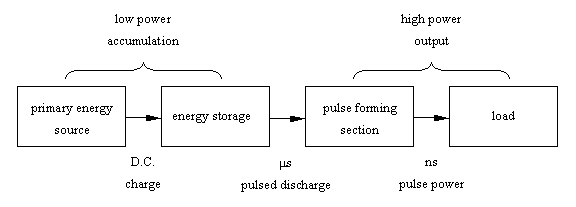
\includegraphics[height=4cm,width=8cm,keepaspectratio=true]{HPMsystem}
 \caption{Primjer ubacivanja slike.}
 \label{fig:prva}
	\end{center}
\end{figure}
\end{verbatim}
Uočite uporabu naredbe \verb|\label| unutar bloka. Na nju se potom u tekstu možemo referencirati pisanjem npr.\ \verb|Na Slici~\ref{fig:prva}| čime \LaTeX{} u tekst uvrsti pripadajući broj slike, kao npr.\ ``Na Slici~\ref{fig:prva} prikazana je osnovna shema HPM sustava.''
Znak \verb|~| iza riječi Slici osigurava točno jedan znak razmaka, što pomaže ukoliko je riječ Slika na kraju retka, da ne razdvoji riječ Slika i pripadajući broj slike.

\begin{figure}[!htbp]
	\begin{center}
 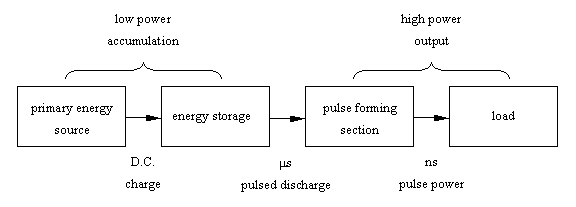
\includegraphics[height=4cm,width=8cm,keepaspectratio=true]{HPMsystem}
 \caption{Primjer ubacivanja slike.}
 \label{fig:prva}
	\end{center}
\end{figure}

Uočite i način prilagođavanja veličine slike. Parametri slike \emph{width} i \emph{height} određuju maksimalne dopuštene dimenzije pri čemu se primarno poštuje manju navedenu dimenziju, a \emph{keepaspectratio} osigurava zadržavanje odnosa dimenzija slike, odnosno sprječava deformaciju slike, nakon proizvoljno unesenih veličina.

Uočite da sve oznake tj.\ \emph{labeli} ne smiju imati razmak u imenu. To vrijedi i općenito, a ne samo za slike.

Također, uočite da nije potrebno pisati ekstenziju slike jer to je uređeno u postavkama glavnoga dokumenta pa time štedi trud. Ekstenzije koje se može izostaviti su: \emph{jpg}, \emph{jpeg}, \emph{png} i \emph{pdf}.

Shema prikazana na Slici~\ref{fig:prva} će biti korištena i za potrebe idućih primjera, a {\color{blue} u mapi na vašem disku ju obrišite nakon što počnete pohranjivati vlastite slike vezane uz vaš rad}.


\section{Ubacivanje podslika}
Ponekada se jedna slika sastoji od dvije ili više podslika kojima želimo opisati neku cjelinu. Slika će dobiti pripadni broj, a podslike slova (a), (b) itd.
To se može postići sljedećom strukturom:
\begin{verbatim}
\begin{figure}[!htpb]
 \begin{center}
  \subfloat[Blok shema HPM sustava.]{\label{fig:HPM}
   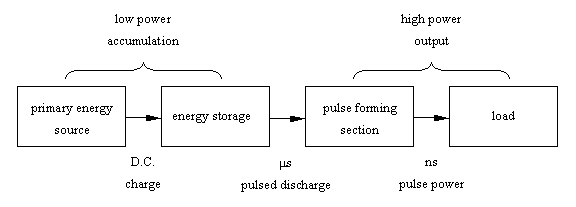
\includegraphics[height=5cm,width=10cm,keepaspectratio=true]{HPMsystem}}\\ 
	    %\hspace{10pt}
   \subfloat[JabRef sučelje za unos ``elektroničke'' reference.]
   {\label{fig:jabref}
   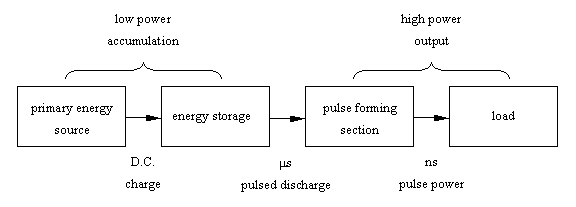
\includegraphics[height=7cm,keepaspectratio=true]{HPMsystem}}
\caption{Primjer ubacivanja više podslika. Ovo je opis cijele slike.}
\label{fig:dvije_podslike}
  \end{center}
\end{figure}
\end{verbatim}
što će uvrstiti ono što se vidi na Slici~\ref{fig:dvije_podslike}, koja se sastoji od dviju podslika.
Podslika~\ref{fig:HPM} pokazuje shemu HPM sustava, a podslika~\ref{fig:jabref} sučelje JabRef programa za unos bibliografskih jedinica.

\begin{figure}[!htpb]
	  \begin{center}
	   \subfloat[Blok shema HPM sustava.]{\label{fig:HPM} 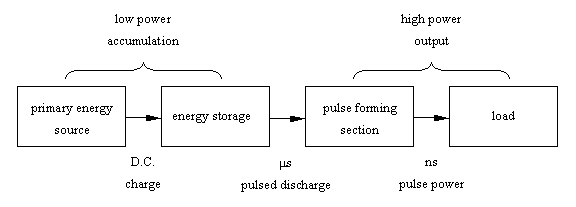
\includegraphics[height=5cm,width=10cm,keepaspectratio=true]{HPMsystem}} \\ %\hspace{10pt}
	   \subfloat[JabRef sučelje za unos ``elektroničke'' reference.]{\label{fig:jabref} 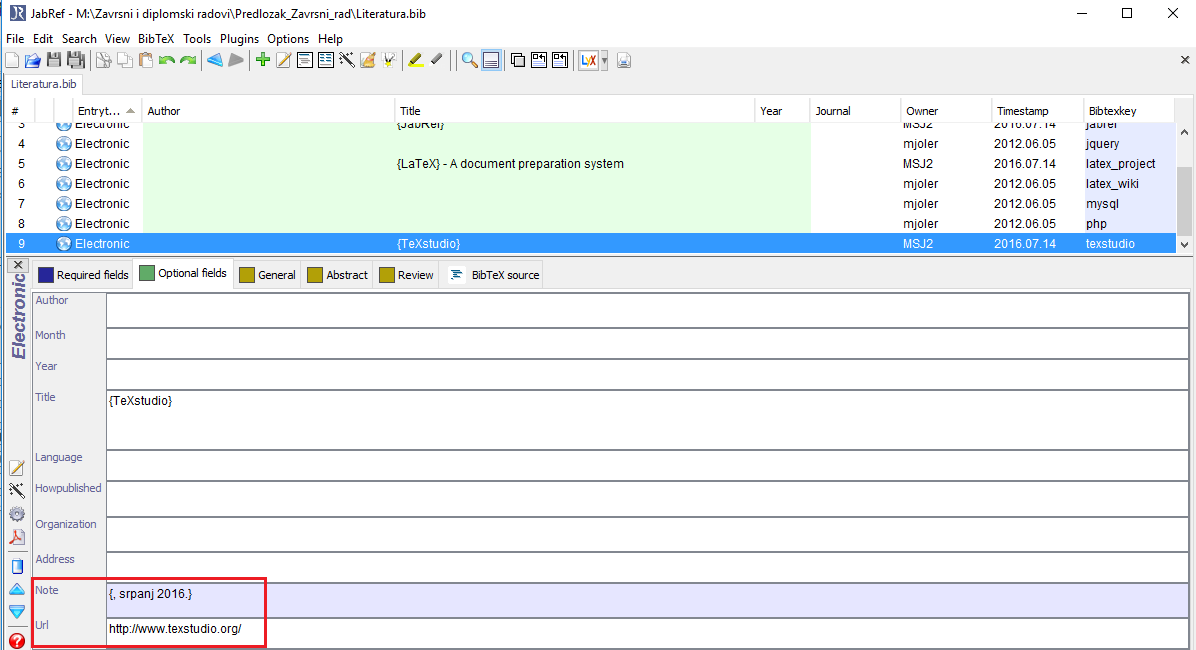
\includegraphics[height=7cm,keepaspectratio=true]{jabref}}
\caption{Primjer ubacivanja više podslika. Ovo je opis cijele slike.}
\label{fig:dvije_podslike}
	  \end{center}
\end{figure}



\section{Ubacivanje tabele} 
Više detalja o kreiranju tabela pročitajte u literaturi, a sljedeći blok vam omogućava kreiranje jednostavne tabele, kao što je prikazano u Tabeli~\ref{tab:prva}.
\begin{verbatim}
\begin{table}[!htbp]
\renewcommand{\arraystretch}{1.2}
\caption{Ovo je primjer izrade tabele.}
\centering
\begin{tabular}{|c|c|c|}
\hline
variabla & vrijednost 1 & vrijednost 2  \\ [0.5ex]
\hline \hline  
A & 5 & 3 \\ [0.5ex] % razmak do iducega retka
B & 4 & 2 \\ [0.5ex]
\hline
\end{tabular}
\label{tab:prva}
\end{table}
\end{verbatim}

\begin{table}[!htbp]
\renewcommand{\arraystretch}{1.2}
\caption{Ovo je primjer izrade tabele.}
\centering
\begin{tabular}{|c|c|c|}
\hline
variabla & vrijednost 1 & vrijednost 2  \\ [0.5ex]
\hline \hline 
A & 5 & 3 \\ [0.5ex] % razmak do iducega retka
B & 4 & 2 \\ [0.5ex]
\hline
\end{tabular}
\label{tab:prva}
\end{table}
%
Podaci koji su u stupcima se u tabeli razdvajaju znakom \&. Novi redak se na kraju aktualnoga retka formira znakom \verb|\\|. Broj stupaca se definira iza \emph{tabular} time što se navedu slova koja označavaju poravnavanje teksta u svakom stupcu, a broj slova znači broj stupaca koji će biti kreiran u tabeli. Vertikalni razmak između redaka u tabeli možete za cijelu tabelu prilagoditi uporabom sljedeće sintakse prije strukture za tabelu:\\
\verb| \renewcommand{\arraystretch}{1.2} | gdje broj u zagradi na kraju (ovdje je 1.2) prilagodite sukladno vašoj preferenciji. Može se prilagoditi i razmak za svaki pojedini redak (uočite \verb|[0.5ex]| na kraju redaka), ali to je manje od interesa jer tipično želimo da svi retci imaju jednaki razmak jedni od drugih.

Slično možete učiniti i za razmak između stupaca tabele navođenjem sljedeće sintakse prije bloka tabele:\\
\verb| \renewcommand{\tabcolsep}{0.3cm} |.



\section{Uporaba kratica u tekstu. Automatsko generiranje popisa kratica.}  \label{sec:kratice}
Listu kratica definirajte u datoteci \verb|Kratice.tex| (vidjeti predložak unutar datoteke). U redovitom tekstu, kraticu  možete ubaciti korištenjem naredbe \verb|\gls{ID_kratice}| gdje je \verb|ID_kraticE| identifikator kratice kako je definiran u datoteci \emph{Kratice.tex}. Pri prvoj uporabi naredbe \verb|\gls|, ispisat će se najprije puni naziv pojma pa u zagradi kratica, a kod svake sljedeće uporabe, ispisat će se samo kratica. Na primjer, kada (nakon prethodnog deklariranja u datoteci \verb|Kratice.tex|) upotrijebite \verb|\gls{gsm}| prvi puta, u tekstu će se ispisati \gls{gsm}, a kada upotrijebite \verb|\gls{gsm}| drugi puta i dalje, u tekstu će se ispisati samo \gls{gsm} (usporedi s definicijom kratice u datoteci \verb|Kratice.tex|). 
 
{\color{red} Listu kratica generirate sljedećim postupkom:} \label{generiranje_liste_kratica}
\begin{enumerate}
	\item Pokrenite kompilaciju cijeloga teksta jedanputa (to će generirati neke datoteke koje su potrebne za daljnju obradu, specifično one s ekstenzijama .ist i .glo).
	\item Otvorite \emph{Command Prompt} aplikaciju na vašem računalu i postavite se u radnu mapu gdje su vam datoteke za diplomski rad. 
	\item Potom pokrenite \emph{makeindex} rutinu (ona će tipično biti već prisutna na vašem računalu) upisujući sljedeću sintaksu: \\
	\verb|makeindex   -s myDoc.ist  -o myDoc.gls   myDoc.glo| \\
	gdje naziv datoteke \emph{myDoc} treba zamijeniti nazivom vaše glavne .tex datoteke, (npr. \verb|JMBAG_Ime_Prezime.tex|).
	\item Pokrenite \LaTeX{} još jednom ili dva puta, ako treba, dok se u uvodu pdf dokumenta ne pojavi lista kratica (pod naslovom \emph{Pojmovnik}).	
\end{enumerate}

Možda isprva zvuči složeno, ali zapravo nije (bar ne uz ovako precizne upute!). Svaki puta kada dodate nove definicije kratica, potrebno je ponoviti ovaj postupak da bi se ažurirale odgovarajuće datoteke i uredno prikazala potpuna lista u pdf-u (a i izbjegle poruke o pogreškama tijekom kompajliranja teksta). 

Nije teško nakon što prvi puta prođete ovaj postupak i omogućava vam u tekstu biti dosljedan u uporabi određene kratice. Da izbjegnete čuđenje, važno je još reći da će se ovim postupkom automatski stvoriti tek lista kratica koje ste u tekstu upotrijebili uporabom sintakse \verb|\gls|, a ne na temelju liste definicija koje ste naveli u datoteci \verb|Kratice.tex|. Zato, ako nijednom u tekstu ne upotrijebite sintaksu \verb|\gls|, neće biti ispisan ni popis kratica tj.\ \emph{Pojmovnik}. {\color{blue} Kako \LaTeX{} na kraju uvijek nagradi trud koji je uložen u savladavanje njegove sintakse, pogodnost ovakvoga automatskoga kreiranja Pojmovnika je i to što uz svaki kraticu \LaTeX{} automatski ispiše i brojeve stranica na kojima se dotična kratica pojavljuje!} U elektroničkom pdf dokumentu, brojevi stranica su ujedno i hiper-veze na te stranice pa se tako može odmah skočiti na stranicu gdje je pojedina kratica upotrijebljena.

Ukoliko vam se prethodno opisani postupak čini presloženim, popis kratica možete napraviti i ručno, isto pomoću datoteke Kratice.tex, u kojoj također postoji kratki predložak i za takav pristup. Za to je onda u osnovnoj datoteci \verb|JMBAG_Ima_Prezime.tex| potrebno deaktivirati liniju koda koja počinje sa \verb|\printglossary|, a aktivirati blok koji počinje sa \verb|\begin{glossary}| i završava sa \verb|end{glossary}|.



\section{Naglašavanje teksta}
\subsection{Navodnici}
Za navodnike s lijeve strane fraze (otvaranje navodnika) koristi se 2x jednostruki navodnik koji se na tipkovnici nalazi lijevo od broja 1, a za navodnike s desne strane fraze (zatvaranje navodnika), koristi se 2x jednostruki navodnik koji se na tipkovnici nalazi na tipki \emph{ć}, što proizvede npr.\ ``abc''.

{\color{blue} Alternativno, u ovom paketu je pripremljena i naredba {\color{red} \verb|\navod{abc}|} gdje je \emph{abc} tekst koji se stavlja između navodnika, tj.\ \navod{abc}.}

\subsection{Kosa i podebljana slova}
Naglašavanje neke riječi ili fraze pomoću kosih (italic) slova možemo dobiti uporabom naredbe {\color{red} \verb|\emph{abc}|} ili pomoću  {\color{red}\verb|\textit{abc}|} gdje je \emph{abc} neki tekst koji se želi naglasiti.

\textbf{Podebljana slova} možemo postići uporabom naredbe {\color{red} \verb|\textbf{abc}|} gdje je \textit{abc} neki tekst koji želimo podebljati.

\section{Verbatim: okruženje za doslovni tekst}
Verbatim okruženje omogućava ispis teksta u izvornom obliku, bez da ga \LaTeX{} tumači po svojiim sintaktičkim pravilima. To je pogodno kada se na stranicu  npr.\ želi kopirati dio programskoga koda iz nekog jezika i kada želimo zadržati sve izvorne znakove u nekoj frazi, bez da \LaTeX{} počne javljati pogreške kod kompajliranja, što bi se moglo pojaviti kada se ne bi koristilo \emph{verbatim okruženje}, pošto bi neke znakove interpretirao kao pogreške u sintaksi.

Postoji kraći i duži oblik verbatima. Kraći služi za kraću frazu od jedne ili par riječi, a duži za više redaka.

\noindent Kraći oblik verbatima ima sintaksu: \verb+\verb|neka fraza|+

\noindent Duži oblik verbatima ima sintaksu:\\
\verb|\begin{verbatim}| \\
\verb|neki tekst| \\
\verb|\end{verbatim}| \\


\section{Kreiranje jedne jednadžbe ili serije jednadžba}

\subsection{Kreiranje jedne jednadžbe}
Jednadžba se napiše u posebnom matematičkom modu koji se kreira pomoću bloka:
\begin{verbatim}
	\begin{equation}
		 A = B + C   \label{eq:prva}
	\end{equation}
\end{verbatim}
što će dati sljedeći izgled:
\begin{equation}
	 A = B + C   \label{eq:prva}
\end{equation}
Da bi se na nju referenciralo, na željenom mjestu u tekstu upišemo \verb|\eqref{eq:prva}|, čime će se uvrstiti njezin pripadni (automatski generirani) broj, a za potpuniji smisao možemo npr.\ napisati \verb| Jednadžba~\eqref{eq:prva}|, rezultat čega je da će u tekstu pisati Jednadžba~\eqref{eq:prva}. 
Ako ju se ne želi numerirati, onda se nakon riječi \emph{begin} stavi zvjezdica, tj.\ \verb|begin*{equation}|.

\subsection{Kreiranje grupe jednadžba}
Grupa jednadžba se kreira uporabom \emph{subequations} sintakse. Na primjer, sljedeći blok će definirati dvije podjednadžbe u grupi, gdje će svaka biti numerirana istim brojem, a razlikovati slovom iza broja.
\begin{verbatim}
	\begin{subequations}
		\begin{align}
		        A &= B + C  	\label{subeq:prva} \\
		        D &= F + G		\label{subeq:druga}
		\end{align}
	\label{subeq:obje}
	\end{subequations}
\end{verbatim}

To će u izlaznom dokumentu rezultirati sljedećim izgledom:
\begin{subequations}
\begin{align}
        A &= B + C  	\label{subeq:prva} \\
        D &= F + G		\label{subeq:druga}
\end{align}
\label{subeq:obje}
\end{subequations}
U \eqref{subeq:prva} je prikazano dobivanje vrijednosti $A$, a u \eqref{subeq:druga} je prikazano dobivanje vrijednosti $D$. Jednadžba~\eqref{subeq:obje} je \emph{čuveni studentov zakon}!



\section{Liste}
Liste su česte forme u tekstu kojima se na pregledni način nabrajaju neke stavke. Stavke obično navodimo ili s točkama na početku, s brojevima ili sa slovima. U \LaTeX-u su upravo ta tri stila unaprijed definirana, a moguće su i složenije definicije stilova i kombinacije lista.

\subsection{Lista s točkama}
Lista s točkama se postigne blokom
\begin{verbatim}
\begin{itemize}
    \item prva nenumerirana stavka
    \item druga nenumerirana stavka
\end{itemize}
\end{verbatim}
što na ekranu proizvede:
\begin{itemize}
% \setlength\itemsep{1ex}   % za lokalnu prilagodbu
	\item prva nenumerirana stavka
	\item druga nenumerirana stavka
\end{itemize}

\subsection{Lista s brojevima}
Numerirana lista s brojevima se postigne blokom
\begin{verbatim}
\begin{enumerate}[itemsep=1ex, topsep=4pt, partopsep=0pt]
     \item prva numerirana stavka
     \item druga numerirana stavka
\end{enumerate}
\end{verbatim}
U uglatoj zagradi su tri parametra kojima se točno može kontrolirati vertikalni razmak između stavki u listi (\emph{itemsep}), razmak između prethodnoga teksta i prve stavke u listi (\emph{topsep}) i dodatni prostor između liste i prethodnoga paragrafa kada lista započinje novi paragraf (\emph{partopsep}), ali te parametre \textbf{ne morate navoditi} tj.\ tu uglatu zagradu ne morate pisati. Tada će se primijeniti vrijednosti parametara koje su definirane za cijeli dokument, a ove parametre se može upotrijebiti tek da u nekom pojedinom slučaju prilagodite razmake.
Za osjetiti efekte ovih parametara, najbolje se malo sam poigrati različitim vrijednostima parametara i vidjeti posljedice toga na listu (pri tome se uz brojeve kao prikladne jedinice za razmak mogu koristiti \emph{pt}, \emph{ex} ili \emph{em}).

\subsection{Proizvoljno označena lista}
Takva se lista može postići u sklopu općenitije forme koja omogućuje proizvoljni opis ispred pojedine stavke, pomoću sljedećega bloka:
\begin{verbatim}
\begin{description}
     \item[a)] prva opisna stavka
     \item[b)] druga opisna stavka
\end{description}
\end{verbatim}
što na ekranu proizvede:
\begin{description}%[itemsep=1ex, topsep=4pt, partopsep=0pt] za lokalnu prilagodbu
	\item[a)] prva opisna stavka
	\item[b)] druga opisna stavka \\
\end{description}
%
Kod ove strukture, u uglatu zagradu iza naredbe \verb|\item|, navodi se proizvoljna oznaka kojom se želi na neki način ``numerirati'' listu.
%:::::::::::::::::::::::::::::::::::::::::::::::::::
\chapter{Dodatne informacije}
\section{Primjeri uporabe sintaktičkih struktura}
\begin{enumerate}
	\item Za uvid u kontekstualnu primjenu raznih sintaktičkih struktura, možete otvoriti datoteku \href{run:Intro.tex}{{\color{blue}Intro.tex}}, unutar koje su napisane i ove upute. 
	\item Primjere složenijih sintaktičkih struktura, kao što su ubacivanje slike, tabele ili jednadžbe, možete naći u datoteci \href{run:sintaksa_cestih_struktura.tex}{{\color{blue}sintaksa\_cestih\_struktura.tex}} koja je dio paketa. Odabrane se strukture može kopirati i zalijepiti u vaš tekst, uz minimalne prilagodbe kao što su naziv slike, veličina slike, opis i ID slike, a analogno i za tabele i jednadžbe.
	\item Konačno, za više detalja o bilo čemu, potražite informacije u dvama priručnicima koji su priloženi u mapi \href{run:prirucnici}{{\color{blue}prirucnici}} ili na webu, gdje se, među obiljem drugih informacija, nalaze i korisne wiki stranice \cite{latex_wiki,tex_exchange} o \LaTeX-u pomoću kojih se obično brzo pronađe upute i zadovoljavajuće rješenje kakvom sintaksom se može urediti željeni dio teksta.
\end{enumerate}

\section{Savjeti za lakše uređivanje teksta}
Vjerujem da vam ovaj dokument može uvelike pomoći u pripremi teksta vašega završnog/diplomskog rada i omogućiti da glavninu vremena trošite na sadržaj rada, a manje na formatiranje rada jer to će za vas sada obaviti \LaTeX{}! 

No, korektnosti radi, potrebno je napomenuti i sljedeće: \LaTeX{} je vrlo osjetljiv na pogreške u sintaksi naredbi (da, baš kao što su i programski jezici) pa vas može povremeno ugnjaviti javljanjem pogreške koju nikako ne uspijevate uočiti gdje je. Iskustvo kojim se izbjegava ta nelagoda jest sljedeće:
\begin{itemize}
	\item svako poglavlje napišite u novoj datoteci (da biste količinu teksta razdvojili na preglednije i manje cjeline) koju imenujte prikladnim imenom (bez razmaka u imenu). Potom te datoteke samo pozivajte iz glavnoga dokumenta \verb|JMBAG_Ime_Prezime.tex| pomoću naredbe \verb|\include{ime_datoteke}|. Takav je pristup upravo i korišten u pripremi ovoga paketa.
	%
	\item {\color{red} budite koncentrirani dok pišete \LaTeX{} naredbe, poglavito zagrade, posebne znakove i matematički tekst gdje se zahtijeva uporaba znaka \$!}
	%
	\item kompajlirajte tekst prije nego se skupi puno teksta jer tako ćete imati manje teksta za prekontrolirati u slučaju pogreške. Također vam za provjeru tek manjega dijela dokumenta može pomoći paket \verb|\usepackage{syntonly}| i naredba \verb|syntaxonly|, a isto tako i naredba \verb|\includeonly{ime_datoteke}| kojom ćete kompajlirati samo tu navedenu datoteku, čime  ispred ``neželjenih'' datoteka ne morate stavljati znak ``komentara'' (\%).
	%
	\item ako niste sigurni hoće li vam raditi neka naredba nakon pisanja, radije tekst kompajlirajte odmah po pisanju te naredbe---da vidite što ćete dobiti i riješite dvojbu, nego da čekate da se skupi još dubioznih mjesta u tekstu, kada će nakon kompajliranja biti teže detektirati koja linija teksta zapravo izaziva probleme (\LaTeX-ov prozor s porukama često nije odveć precizan u lociranju i opisu pogrešaka, ovisno o editoru teksta koji koristite).
\end{itemize}


\section{Završne napomene}
Ovime zaključujemo uvodne upute koje će najvećem broju studenata biti dovoljne (ili barem dovoljna osnova) za uspješno pisanje završnog odnosno diplomskog rada.

Prije nego prijeđete na kreiranje vlastitoga sadržaja učinite još sljedeće akcije kojima ćete deaktivirati dio paketa koji će biti nepotreban:
\begin{enumerate}
	\item u mapi \href{run:slike}{{\color{blue}slike}}, obrišite datoteke \verb|HPMsystem.png| i \verb|jabref.png| jer su one služile tek za ilustracije u ovim Uputama.
	%
	\item u glavnoj datoteci  \href{run:JMBAG\_Ime\_Prezime.tex}{{\color{blue}JMBAG\_Ime\_Prezime.tex}} stavite znak komentara ``\%'' ispred linije \verb|
\chapter{Kako koristiti paket za pisanje završnoga rada u \LaTeX-u}
Ovo su uvodne napomene za korištenje predloška za pisanje završnoga ili diplomskoga rada studenata Tehničkoga fakulteta u Rijeci. Prije korištenja paketa, pročitajte ovaj tekst jer će vam dati nužne uvodne informacije, znatno vam olakšati i ubrzati uređivanje teksta nakon toga, pri čemu će vas i voditi kroz uporabu ovoga paketa na praktičan način.

Paket je pripremljen tako da student što prije može pisati vlastiti tekst u već pripremljenom predlošku koji će, uz minimalno učenje sintakse \LaTeX-a, studentu olakšati urediti svoj rad. U paketu su uključene potrebne upute i sintaktičke strukture koje bi trebale udovoljiti potrebama većine studenta, a dodatne informacije postoje u dvama priručnicima koji su uključeni u ovom paketu te, naravno, na raznim web stranicama na internetu koje su posvećene \LaTeX-u (vidi u nastavku).

{\color{red} POZOR: paket treba biti prekopiran negdje na disk ne mijenjajući originalnu strukturu mapa (foldera) i ne mijenjajući nazive datoteka koje su u mapi \emph{tex\_aux}!}


\section{Opis sadržaja paketa}
\vspace{-2ex}
Paket se sastoji od:
\begin{itemize}
 \item datoteke \href{run:UPUTE.pdf}{{\color{blue} UPUTE.pdf}} koja sadrži postupak instalacije potrebnih alata na računalo te korištenja paketa. \emph{UPUTE} su bazirane na Windows OS, a korisnici drugih OS-ova si na naznačenim web lokacijama samo trebaju naći instalacije za njihov OS.
 %
 \item datoteke \verb|JMBAG_Ime_Prezime.tex| koja je središnja datoteka koja povezuje sve cjeline i kompajliranjem koje se dobije izlazni \verb|JMBAG_Ime_Prezime.pdf| dokument (naravno, tijekom rada, upisat ćete svoj specifični JMBAG i ime i prezime).\\ U ovoj se datoteci inicijalno nalaze i upute za korištenje paketa kao i primjeri osnovne uporabe najčešćih sintaktičkih struktura u \LaTeX-u koje bi trebale biti dovoljne većini studenata za pisanje rada.
 %
 \item mape \verb|tex_aux| u kojoj su \emph{interne datoteke} koje definiraju stilove, formate i sl.\ koji služe u slaganju izlaznoga formata. \textbf{Student/ica s njima ne treba \emph{ništa} raditi}, ali one trebaju biti u \verb|tex_aux| mapi pod glavnom mapom završnoga rada, kao što je postavljeno u ovom paketu.
 %
 \item mape \emph{slike} u koju student treba pohraniti sve slike koje će koristiti u radu. Ime mape se ne smije preimenovati bez boljega poznavanja sintakse \LaTeX-a jer ovaj paket da bi ispravno radio očekuje baš takvo ime mape!
 %
 \item datoteke \verb|sintaksa_cestih_struktura.tex| koja ne sudjeluje izravno u kompajliranju pdf dokumenta, nego služi kao repozitorij u kojemu su sadržane najčešće potrebne sintaktičke strukture koje su spremne za kopiranje u vaš tekst uz minimalnu prilagodbu parametara (npr.\ opis slike, ime datoteke specifične slike koju se ubacuje i proizvoljni ID te slike za kasnije referenciranje).
 %
 \item mape \href{run:prirucnici}{{\color{blue}prirucnici}} u kojoj se nalazi nekoliko najpopularnijih priručnika za uporabu \LaTeX-a. 
\end{itemize}
%%%%%%%%%%%%%%%%%%%%%%%%%%%%%%%%%%%%%%%%%%%%%%%%%%%%%%%%%%%%%%%
\section{Čime se opremiti za pisanje rada}
Da bi se rad napisao pomoću \LaTeX-a (a to vrijedi svake lipe!), najprije je na računalo potrebno instalirati:
\begin{enumerate}
	\item obavezno: \LaTeX{} software 
	\item obavezno: editor za uređivanje teksta 
	\item neobavezno, ali korisno: softver za opis literature. (Premda dodatni softver nije nužan jer se popis literature može obraditi i ručno (no to je manje sofisticirano kod uvrštavanja referenca), sugeriram instalaciju softvera koji pomoću intuitivnih sučelja korisniku omogućava opis pojedine korištene literature (kao mala baza podataka), a potom se pojedina jedinica literature jednostavno ubacuje u tekst, a popis literature se na kraju automatski formira (više o tome pročitajte u nastavku).
\end{enumerate}

\subsection{Instalacija \LaTeX-a}
\begin{enumerate}
	\item odite na središnji \LaTeX{} portal \cite{latex_project}: \url{http://www.latex-project.org/}
	\item kliknite na poveznicu \href{http://www.latex-project.org/ftp.html}{Getting LaTeX} i potom uočite i povucite instalaciju koja odgovara vašem OS-u (npr.\ proTeXt za Windows, MacTeX za Mac, TeX Live za Linux). Pozor: instalacijski paket je velik i može duže potrajati čak i na brzoj vezi---dajte si dovoljno vremena za obaviti download.
	\item Instalirajte \LaTeX{} slijedeći upute koje su priložene za odabranu instalaciju (npr.\ proTeXt za Windowse daje kratki pdf s uputama koje vas vode kroz instalaciju korak po korak).
\end{enumerate}

\subsection{Instalacija editora teksta}
Instalirajte editor koji je pogodan za pisanje \LaTeX{} koda. \textbf{Za Windows OS, toplo preporučam}  \href{http://www.texstudio.org}{{\color{blue} TeXstudio}} \cite{texstudio} jer je bogat opcijama, ugodan za rad i stabilan, a instalacije postoje i za Linux i Mac OS. TeXstudio se zasebno povuče i instalira na računalo, a neke editore teksta koji već dođu u paketu za instalaciju LaTeXa možete ignorirati (npr.\ za Windows je do nedavno bio popularan \emph{TeXnicCenter} i dolazi već upakiran u proTeXt-u (a možda ćete naći i \emph{TeXworks}), za Mac je kvalitetan \emph{TeXShop} koji sada također dolazi u paketu s MacTeX-om). 

\label{encoding1} {\color{red} POZOR: Premda će ovo biti još napomenuto na stranici~\pageref{encoding2}, prije samoga početka pisanja vašega rada, što prije želim napomenuti sljedeći važni detalj: za svaki vaš tekst koji pišete u editoru teksta, uvjerite se da je kodna stranica postavljena na \navod{windows-1250}, što je ključno da bi se u izlaznom pdf-u ispravno ispisivali hrvatski dijakritički znakovi! U TeXstudiu, aktualnu kodnu stranicu se može vidjeti i promijeniti preko maloga izbornika u doljnjem desnom kutu glavnoga prozora, gdje se nalazi opcija ``Encoding''. Ukoliko tu ne piše ``windows-1250'', kliknite na izbornik, odaberite opciju ``More Encodings'' pa u potom otvorenom sučelju odaberite kodnu stranicu ``windows-1250 / CP 1250'' i potvrdu sa ``Change To''.}

\subsection{Instalacija programa za opis korištene literature}
\emph{Ponavljamo: Korištenje BiBTeX programa za opis literature \textbf{nije} neophodno, ali jest korisno. U datoteci po imenu \href{run:Literatura.tex}{{\color{blue}Literatura.tex}}, koja je uključena u ovaj paket, već su namještene postavke kao da će se literatura opisati pomoću BiBTeX programa (npr.\ JabRef-a) i ne treba ništa mijenjati, ali ispod toga se može pronaći i upute i za drugi--ručni-- način (p)opisivanja literature.}

Kao bibtex program za opis literature, preporučam \href{http://www.jabref.org}{{\color{blue} JabRef}} program \cite{jabref}. To je legalno besplatno dostupni program za Windows OS (ali postoji i za Mac, a i platformski neovisna instalacija) koji nam omogućava opisivanje literature na lak način pomoću intuitivnih sučelja, a kao rezultat kreira \emph{BibTeX} datoteku \emph{Literatura.bib} (gdje je (\emph{Literatura} naziv koji korisnik treba dodijeliti pri pohrani JabRef datoteke na disk u slučaju ovoga predloška, da bi paket funkcionirao) u kojoj je literatura opisana na način koji \LaTeX{} razumije. 

Uočite da ako ne koristite JabRef, već se odlučite za ručni unos literature, što se isprva doima jednostavnijim, tada će vam redoslijed referenca u popisu literature odgovarati točno redoslijedu koji ste naveli u tom popisu --- dakle morate paziti da redoslijed formirate onim redom kojim pozivate reference u vašem tekstu (što kod nekog kasnije ubacivanja dodatne reference unutar već postojećega redoslijeda traži brigu da ju se ubaci na odgovarajuće mjesto u popisu literature), a također trebate paziti i na formatiranje teksta svake reference! 

Za razliku od toga, korištenjem JabRef-a, izbjegavate ručno formiranje popisa literature i ne trebate brinuti o redoslijedu referenca, već samo pomoću JabRefa trebate unijeti sve jedinice literature koju ćete navesti, a \LaTeX{} će vam automatski formirati listu referenca onim redoslijedom kojim reference bude pozivali u tekstu!

Nakon što kompajlirate projekt, stvorit će vam se pomoćna datoteka imena \href{run:JMBAG_Ime_Prezime.bbl}{{\color{blue}JMBAG\_Ime\_Prezime.bbl}} u kojoj će jedinice literature tijekom kompilacije biti formatirane i odatle se ubacuju u konačnu verziju teksta. Stoga, \textbf{ukoliko ima ikakvih detalja koje u opisu literature treba prilagoditi, a ne možete automatskim putem}, uvijek vam kao ``zadnja crta obrane'' ostaje otvoriti \verb|bbl| datoteku i tamo ručno napraviti izmjene. Potom ponovo kompajlirajte projekt i te će se promjene vidjeti u pdf-u tj.\ ručno unijete promjene neće biti poništene sve dok ne obrišete cijelu datoteku.

Umjesto da rukom pišete cijelu bibliografiju, vremenski vam je vjerojatno učinko\-vitije popis literature generirate uporabom JabRef-a, a potom ako išta još treba prilagoditi, onda samo to napraviti ručno u \verb|bbl| datoteci.


\subsubsection{Osnovna uporaba JabRef programa}
Upoznajte se s najvažnijim opcijama u \emph{JabRef}-u:
\begin{itemize}
	\item uočite ikonu (pod znakom ``+'' i tekstom \emph{New BibTeX Entry}) za unos nove jedinice literature (npr. knjige, članka, web portala i sl.)
	%
	\item kada kliknete za unos nove stavke literature, uočite kakvi se sve tipovi literature nude za odabir. Odabirom opcije koja odgovara naslovu koji želite unijeti, otvorit će vam se novi prozor s poljima u koja se može unijeti informacije o literaturi. Za odabrani tip literature samo su neka polja obavezna (nalaze se pod karticom (eng.\ \emph{tabom}) \emph{Required fields}), dok se pod drugim karticama može i ne mora unijeti dodatne informacije. U slučaju naših završnih/diplomskih radova, bit će znatan udjeli literature koja je na internetu pa za formatiranje iste, pročitajte upute i napomene u nastavku ove sekcije.
	%
	\item kada je više autora, njihova imena se u JabRefu polju za unos autora razdvajaju pisanjem ključne riječi \verb|and| (a ne razmakom, zarezom ili točka-zarezom!)
	%
	\item U popisu literature se neće uvijek pojam prepisati onako kako ste ga vi zapisali u JabRefu! To je posljedica stilova koji su definirani u \verb|bst| datoteci (ne zamarajte se time sada jer je za naprednu razinu \LaTeX-a). No, ako neki pojam baš ne ispadne suvislo napisan u popisu literature ili baš želite forsirati određeni način zapisa (često slučaj kada se riječ s velikim slovima ne interpretira onako kako želite), tada točno određeni zapis možete forsirati na način da \verb|{tu riječ ili frazu stavite unutar vitičastih zagrada}|
	%
	\item prije nego pohranite pojedinu stavku pomoću \emph{Ctrl+S}, \textbf{morate svakoj jedinici literature dodijeliti jedinstveni identifikator}, tzv.\ \emph{Bibtexkey}, što je jedno od polja koja su obavezna za unos. Možete ručno upisati neki proizvoljni string, ali pogodnije je generirati ga automatski.\\ Za to učiniti među ikonama na vrhu imate ikonu koja izgleda kao (čarobni) štapić sa zvjezdicama oko njega, klikom na kojega \emph{JabRef} automatski dodijeli jedinstveni BibTeX \emph{ključ} za tu bibliografsku jedinicu. Pomoću toga ključa se poslije bilo kada i bilo gdje u pisanju vašega rada možete pozvati na tu referencu, a \LaTeX{} će sve ostalo obaviti za vas tj.\ dodijeliti joj odgovarajući broj u tekstu i s tim brojem uvrstiti u popis literature.
	%
	\item korisnik ima mogućnost i promijeniti uzorak po kojem se kreira struktura automatski generiranoga jedinstvenoga BibTeX ključa tako da se otvori opcija izbornika \emph{Options $>>$ Preferences $>>$ BibTeX key generator}, gdje je na vrhu prozora prikazan \emph{default} uzorak, npr. \verb|[auth]:[year]| što znači da se ključ kreira na bazi \verb|prezime(autora):godina(rada)|. To se sada može urediti po nekom novom uzorku, no ovako definirani uzorak u biti zadovoljava, a ako igdje ima potrebe za dodatnim razlikovanjem, može se na automatski generiranom ključu još ručno napraviti korekcija dodavanjem nekog znaka na kraju, kao npr.\ dodavanjem \verb|_a| i sl. (Klikom na karticu \emph{BibTeX source} možete vidjeti kako će unos vaših podataka zapravo biti zapisan u vašoj \emph{Literatura.bib} datoteci koja će se formirati od svih bibliografskih jedinica koje unesete.)
	%
	%
	\item Za \emph{ime} vaše bibliografske datoteke kod pohrane na disk obavezno upišite  \emph{Literatura} jer to ime očekuje ovaj paket. Pozor: Datoteka \emph{Literatura.bib}, koju ste tako kreirali, mora se nalaziti unutar mape ovoga paketa da bi sve ispravno radilo! U paketu je za primjer već kreirana jedna datoteka istoga imena koju za vježbu student može i otvoriti u \emph{JabRef}-u, ali to su samo pokazne bibliografske jedinice unesene kao primjer, koje student treba u konačnici zamijeniti svojim bibliografskim jedinicama.
	%
	\item Za ``elektroničke'' izvore literature (tj.\ sve što ste kao informaciju našli na webu), JabRef nudi tip literature pod nazivom ``Electronic'' (vidi Sl.~\ref{fig:jabref}). U njemu pod karticom (eng.\ tabom) \emph{Optional fields} pod poljem \verb|Title| možete upisati ime web stranice (autor, tvrtka i sl.), pod poljem \verb|url| možete upisati URL adresu te web stranice, a pod poljem \verb|Note| upisati datum kada ste posjetili tu web stranicu (npr.\ \emph{srpanj 2016.} ili \emph{3.~rujna~2016.}). Rezultat toga će u pdf-u biti da je sve napisano redoslijedom koji je predviđen u Uputama RiTeha za pisanje diplomskog rada \cite{riteh_upute}, \emph{osim što u ovom Predlošku do sada nisam uspio riješiti ubacivanje zareza između URL adrese i datuma posjeta toj URL adresi}, koji bi ta dva podatka odvojio, pa je tu potrebna mala ručna \emph{prilagodba na jedan od ovih dvaju načina}:
	\begin{enumerate}[label=\textbf{\roman*)}]
		\item kod unosa datuma u polje \verb|Note| (u sučelju JabRef-a), upišite datum na sljedeći način: \verb|{, <datum>}|, gdje je \verb|<datum>| vaš specifični datum, dok će \emph{zarez} iza prve zagrade izvršiti razdvajanje URL adrese i datuma, a \textbf{vitičaste zagrade} osigurati da se to baš tako točno prenese u pdf-dokument (uključujući i da se mjesec napiše malim početnim slovom, što inače ne bi bio slučaj). (Za neke druge tipove referenca kao npr.\ tip \emph{manual}, zarez vam prije datuma neće trebati jer će naziv literature završiti zarezom.) U Jabrefu vam i inače vrijedi da kada želite forsirati da se pojam baš točno u popisu literature zapiše onako kao ste htjeli, onda se pojam stavi unutar vitičastih zagrada \verb|{kao u ovom primjeru}|.
		\item ako u polju \verb|Note| ne upišete datum na prethodno opisani način, onda vam u pdf dokumentu neće biti upisan zarez između URL adrese i datuma koji ste unijeli, a također će i mjesec biti napisan velikim početnim slovom (što nije strašno, ali je manje poželjno). To možete \emph{ručno} prilagoditi tako da otvorite \verb|.bbl| datoteku i pomoću \emph{Find/Replace} operacije sve nazive mjeseca zamijenite na način da počinju malim početnim slovom (što nije teško kada vam je većina datuma u popisu literature navedena u istom mjesecu), ali zareze ćete svakako morati ubacivati ručno u svaku pojedinu stavku literature jer neće biti nekog predloška kojim biste to riješili automatski pomoću \emph{Find/Replace} operacije. Na kraju opet kompajlirajte projekt. S obzirom na navedeno, prvi način je vremenski štedljiviji!
	\end{enumerate}
\end{itemize}

%%%%%%%%%%%%%%%%%%%%%%%%%%%%%%%%%%%%%%%%%%%%%%%%%%%


\chapter{Primjeri najčešćih sintaktičkih struktura}
Prije stvarnoga početka pisanja svoga rada, upoznajte se s osnovnim sintaktičkim strukturama koje će vam trebati tijekom pisanja rada.

U nastavku su opisane najčešće sintaktičke strukture (dio njih možete naći i u datoteci \emph{Intro.tex}), a dodatne složenije strukture su pohranjene u datoteci \href{run:sintaksa_cestih_struktura.tex}{{\color{blue}sintaksa\_cestih\_struktura.tex}} koja je sastavni dio glave mape ovoga paketa. 

\section{Postavljanje naslova poglavlja i sekcija}
\begin{itemize}
	\item \verb|\chapter{Naslov poglavlja}|: za definiranje naslova poglavlja
	\item \verb|\section{Naslov sekcije}|: za definiranje naslova sekcije unutar poglavlja
	\item \verb|\subsection{Naslov podsekcije}|: za definiranje naslova podsekcije
\end{itemize}


\section{Reference na literaturu} \label{sec:RefLit}
Za referencu na pojedini korišteni izvor informacije (tj.\ jedinicu literature), koristimo naredbu \\
\verb|\cite{bibtexkey}|, gdje je \emph{bibtexkey} jedinstveni ključ kojim prethodno označimo tu jedinicu literature. \verb|Bibtexkey| možemo definirati na jedan od sljedećih načina:
\begin{description}
	\item[I)] ako popis literature definiramo izravno u datoteci \href{run:Literatura.tex}{{\color{blue}Literatura.tex}} (opcija (I) u datoteci), onda ispred svake stavke literature treba definirati i jedinstveni \verb|bibtexkey| pomoću naredbe \verb|\bibitem{bibtexkey}| (vidi predložak u datoteci)
	\item[II)] ako literaturu opisujemo pomoću JabRef datoteke \emph{Literatura.bib} (opcija (II) u datoteci), onda se tamo uz svaku stavku definira \verb|bibtexkey| (bude na dnu JabRef obrasca za upis pojedine jedinice literature)
\end{description}
%
Npr.\ ako negdje u tekstu napišemo \verb|\cite{latex_wiki}|, gdje je \verb|latex_wiki| prethodno definirani \emph{bibtexkey}, tada će se u tekstu u uglatoj zagradi pokazati broj  te bibliografske jedinice pod kojim se nalazi u popisu literature (Bibliografiji) na kraju rada (u ovom primjeru, to je broj \cite{latex_wiki}).


\section{Referenca na sekciju, sliku, tabelu ili stranicu} \label{sec:RefText}

Za referenciranje na pojedine dijelove teksta unutar rada, koristimo
{\color{red} \verb|\label{ID}|} i {\color{red} \verb|\ref{ID}|} na način da se \verb|\label{ID}| postavi uz dio teksta koji želimo označiti internom oznakom i poslije ćemo se u tekstu na to referencirati, a \verb|\ref{ID}| upotrijebimo na mjestu s kojega se referenciramo na dio teksta koji je ranije označen pomoću \verb|\label{ID}|.

Ako se želimo referencirati na specifičnu sliku ili tabelu ili sekciju ili jednadžbu u tekstu, tada unutar bloka toga sadržaja stavimo oznaku \verb|\label{prefiks:ID_objekta}| gdje je \emph{objekt} slika ili tablica ili sekcija teksta ili jednadžba, a na željenom mjestu u tekstu se na to referiramo pomoću \verb|\ref{prefiks:ID_objekta}| (u slučaju referenciranja jednadžbe, bolji oblik naredbe je {\color{red} \verb|\eqref{prefiks:ID_objekta}|}).

\verb|ID_objekta| je proizvoljni string (bez razmaka) koji dodijelimo objektu od interesa, a radi preglednijega uređivanja teksta, uobičajeno je u \LaTeX-u za pojedine tipove oznaka staviti i odgovarajući \emph{prefiks}, kao npr.\ \emph{sec} za oznaku sekcije, \emph{fig} za oznaku slike, \emph{tab} za oznaku tabele, \emph{eq} za oznaku jednadžbe i sl. (Tako bi za sliku kojoj dodijelimo $ID=prva$ bilo \verb|\label{fig:prva}|, za tablicu \verb|\label{tab:prva}|, za sekciju \verb|\label{sec:prva}|, a za jednadžbu \verb|\label{eq:prva}|.)

Za referencirati se na \emph{stranicu} u tekstu gdje se nalazi nešto na što se želite osvrnuti, koristi naredba {\color{red} \verb|\pageref{prefiks:ID_objekta}|}. Za njenu primjenu se također prethodno treba označiti željeni tekst pomoću naredbe \verb|\label|.

Tako npr.\ možemo staviti da je primjer kreiranja tabele \emph{prva} opisan na stranici~\verb|\pageref{tab:prva}|, što će za rezultat imati tekst u kojem piše ``da je primjer kreiranja tabele \emph{prva} opisan na stranici~\pageref{tab:prva}'' (jer se u tekstu ta tabela nakon kompajliranja npr.\ nađe na stranici 12). Kako god se tekst smanjivao ili povećavao i navedena tablica mijenjala broj stranice na kojoj se u konačnici nalazi, mi ne moramo o tome brinuti jer \LaTeX{} brine o tome i na kraju napiše točni broj stranice! (To je još jedna o pogodnosti zbog čega se ljudi i odluče, uz nešto početnoga truda, za korištenje \LaTeX-a!).



\section{Poveznica na neki dokument ili URL adresu}
Naredbe \verb|\url| i \verb|\href| služe za kreiranje poveznice na neku URL adresu ili neki dokument na disku.

{\color{red}\verb|\url{adresa}|} će otisnuti URL adresu točno onako kako je \emph{adresa} navedena unutar zagrada.

{\color{red}\verb|\href{akcija:destinacija}{opis}|} će na papiru/ekranu ispisati tekst \emph{opis} koji je naveden u drugoj zagradi, i izvršiti \emph{akciju} prema \emph{destinaciji} koja je navedena u prvoj zagradi. 
\emph{Akcija} može npr.\ glasiti \emph{run} ili \emph{mailto}, gdje će prvi oblik otvoriti mapu ili datoteku staza koje je navedena kao \emph{destinacija}, a drugi oblik pokrenuti pisanje emaila prema email adresi koja je navedena kao \emph{destinacija}.

Ne pretjerujte ipak s uporabom ovih struktura, odnosno uopće ne morate to koristiti u radu, nego za vanjske reference koristiti samo \verb|\cite{bibtexkey}| naredbu, a za unutrašnje reference (na dijelove teksta) kombinaciju naredbi \verb|\label{ID}| i \verb|\ref{ID}| kako je to opisano u Sekciji~\ref{sec:RefText}. 


\section{Ubacivanje slike}
Sliku možemo ubaciti pomoću sljedećega bloka naredbi:
\begin{verbatim}
\begin{figure}[!htbp]
	\begin{center}
 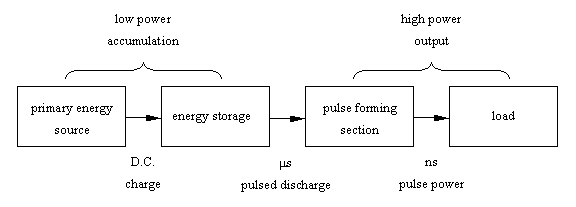
\includegraphics[height=4cm,width=8cm,keepaspectratio=true]{HPMsystem}
 \caption{Primjer ubacivanja slike.}
 \label{fig:prva}
	\end{center}
\end{figure}
\end{verbatim}
Uočite uporabu naredbe \verb|\label| unutar bloka. Na nju se potom u tekstu možemo referencirati pisanjem npr.\ \verb|Na Slici~\ref{fig:prva}| čime \LaTeX{} u tekst uvrsti pripadajući broj slike, kao npr.\ ``Na Slici~\ref{fig:prva} prikazana je osnovna shema HPM sustava.''
Znak \verb|~| iza riječi Slici osigurava točno jedan znak razmaka, što pomaže ukoliko je riječ Slika na kraju retka, da ne razdvoji riječ Slika i pripadajući broj slike.

\begin{figure}[!htbp]
	\begin{center}
 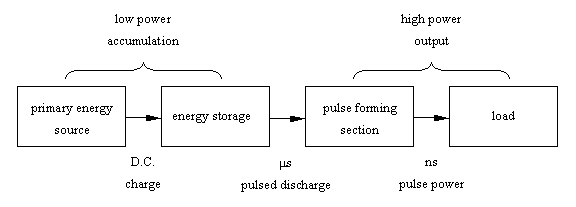
\includegraphics[height=4cm,width=8cm,keepaspectratio=true]{HPMsystem}
 \caption{Primjer ubacivanja slike.}
 \label{fig:prva}
	\end{center}
\end{figure}

Uočite i način prilagođavanja veličine slike. Parametri slike \emph{width} i \emph{height} određuju maksimalne dopuštene dimenzije pri čemu se primarno poštuje manju navedenu dimenziju, a \emph{keepaspectratio} osigurava zadržavanje odnosa dimenzija slike, odnosno sprječava deformaciju slike, nakon proizvoljno unesenih veličina.

Uočite da sve oznake tj.\ \emph{labeli} ne smiju imati razmak u imenu. To vrijedi i općenito, a ne samo za slike.

Također, uočite da nije potrebno pisati ekstenziju slike jer to je uređeno u postavkama glavnoga dokumenta pa time štedi trud. Ekstenzije koje se može izostaviti su: \emph{jpg}, \emph{jpeg}, \emph{png} i \emph{pdf}.

Shema prikazana na Slici~\ref{fig:prva} će biti korištena i za potrebe idućih primjera, a {\color{blue} u mapi na vašem disku ju obrišite nakon što počnete pohranjivati vlastite slike vezane uz vaš rad}.


\section{Ubacivanje podslika}
Ponekada se jedna slika sastoji od dvije ili više podslika kojima želimo opisati neku cjelinu. Slika će dobiti pripadni broj, a podslike slova (a), (b) itd.
To se može postići sljedećom strukturom:
\begin{verbatim}
\begin{figure}[!htpb]
 \begin{center}
  \subfloat[Blok shema HPM sustava.]{\label{fig:HPM}
   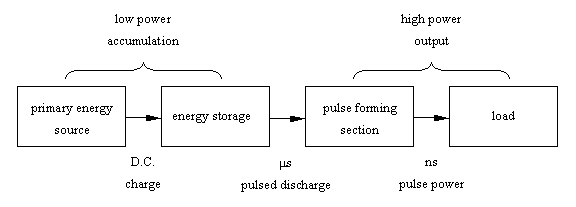
\includegraphics[height=5cm,width=10cm,keepaspectratio=true]{HPMsystem}}\\ 
	    %\hspace{10pt}
   \subfloat[JabRef sučelje za unos ``elektroničke'' reference.]
   {\label{fig:jabref}
   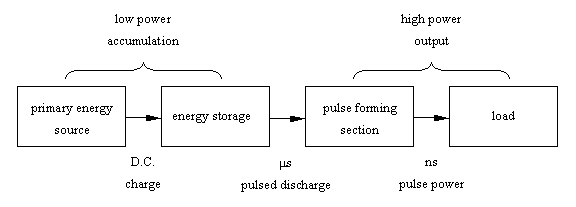
\includegraphics[height=7cm,keepaspectratio=true]{HPMsystem}}
\caption{Primjer ubacivanja više podslika. Ovo je opis cijele slike.}
\label{fig:dvije_podslike}
  \end{center}
\end{figure}
\end{verbatim}
što će uvrstiti ono što se vidi na Slici~\ref{fig:dvije_podslike}, koja se sastoji od dviju podslika.
Podslika~\ref{fig:HPM} pokazuje shemu HPM sustava, a podslika~\ref{fig:jabref} sučelje JabRef programa za unos bibliografskih jedinica.

\begin{figure}[!htpb]
	  \begin{center}
	   \subfloat[Blok shema HPM sustava.]{\label{fig:HPM} 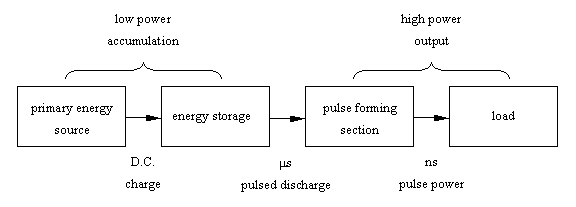
\includegraphics[height=5cm,width=10cm,keepaspectratio=true]{HPMsystem}} \\ %\hspace{10pt}
	   \subfloat[JabRef sučelje za unos ``elektroničke'' reference.]{\label{fig:jabref} 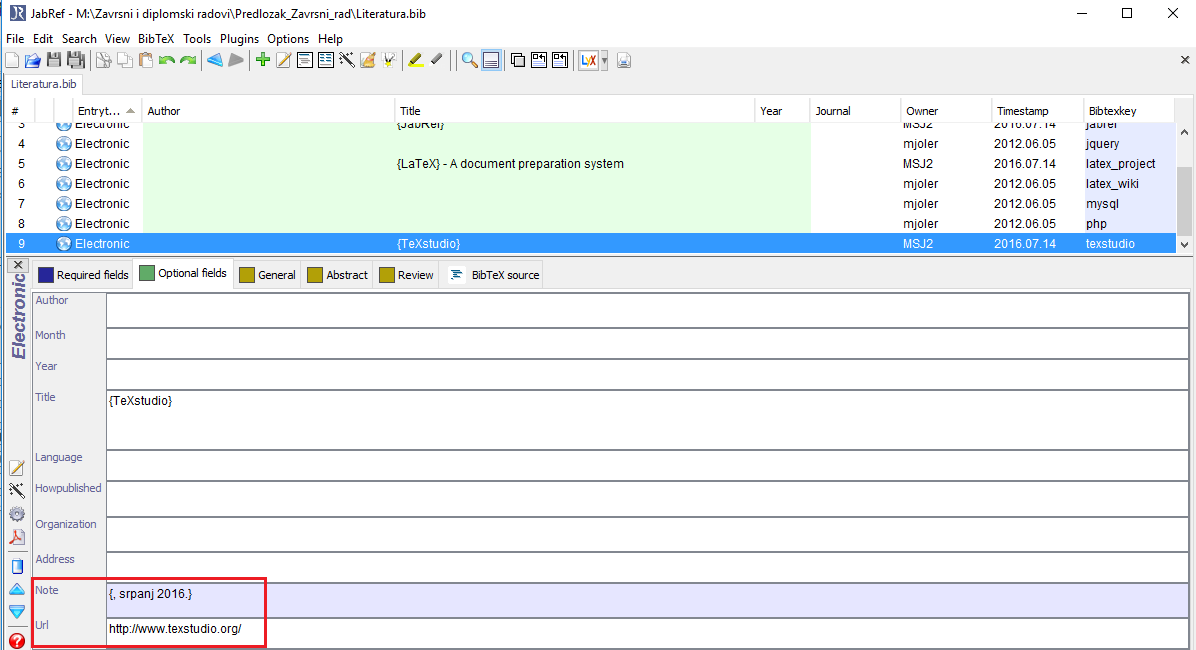
\includegraphics[height=7cm,keepaspectratio=true]{jabref}}
\caption{Primjer ubacivanja više podslika. Ovo je opis cijele slike.}
\label{fig:dvije_podslike}
	  \end{center}
\end{figure}



\section{Ubacivanje tabele} 
Više detalja o kreiranju tabela pročitajte u literaturi, a sljedeći blok vam omogućava kreiranje jednostavne tabele, kao što je prikazano u Tabeli~\ref{tab:prva}.
\begin{verbatim}
\begin{table}[!htbp]
\renewcommand{\arraystretch}{1.2}
\caption{Ovo je primjer izrade tabele.}
\centering
\begin{tabular}{|c|c|c|}
\hline
variabla & vrijednost 1 & vrijednost 2  \\ [0.5ex]
\hline \hline  
A & 5 & 3 \\ [0.5ex] % razmak do iducega retka
B & 4 & 2 \\ [0.5ex]
\hline
\end{tabular}
\label{tab:prva}
\end{table}
\end{verbatim}

\begin{table}[!htbp]
\renewcommand{\arraystretch}{1.2}
\caption{Ovo je primjer izrade tabele.}
\centering
\begin{tabular}{|c|c|c|}
\hline
variabla & vrijednost 1 & vrijednost 2  \\ [0.5ex]
\hline \hline 
A & 5 & 3 \\ [0.5ex] % razmak do iducega retka
B & 4 & 2 \\ [0.5ex]
\hline
\end{tabular}
\label{tab:prva}
\end{table}
%
Podaci koji su u stupcima se u tabeli razdvajaju znakom \&. Novi redak se na kraju aktualnoga retka formira znakom \verb|\\|. Broj stupaca se definira iza \emph{tabular} time što se navedu slova koja označavaju poravnavanje teksta u svakom stupcu, a broj slova znači broj stupaca koji će biti kreiran u tabeli. Vertikalni razmak između redaka u tabeli možete za cijelu tabelu prilagoditi uporabom sljedeće sintakse prije strukture za tabelu:\\
\verb| \renewcommand{\arraystretch}{1.2} | gdje broj u zagradi na kraju (ovdje je 1.2) prilagodite sukladno vašoj preferenciji. Može se prilagoditi i razmak za svaki pojedini redak (uočite \verb|[0.5ex]| na kraju redaka), ali to je manje od interesa jer tipično želimo da svi retci imaju jednaki razmak jedni od drugih.

Slično možete učiniti i za razmak između stupaca tabele navođenjem sljedeće sintakse prije bloka tabele:\\
\verb| \renewcommand{\tabcolsep}{0.3cm} |.



\section{Uporaba kratica u tekstu. Automatsko generiranje popisa kratica.}  \label{sec:kratice}
Listu kratica definirajte u datoteci \verb|Kratice.tex| (vidjeti predložak unutar datoteke). U redovitom tekstu, kraticu  možete ubaciti korištenjem naredbe \verb|\gls{ID_kratice}| gdje je \verb|ID_kraticE| identifikator kratice kako je definiran u datoteci \emph{Kratice.tex}. Pri prvoj uporabi naredbe \verb|\gls|, ispisat će se najprije puni naziv pojma pa u zagradi kratica, a kod svake sljedeće uporabe, ispisat će se samo kratica. Na primjer, kada (nakon prethodnog deklariranja u datoteci \verb|Kratice.tex|) upotrijebite \verb|\gls{gsm}| prvi puta, u tekstu će se ispisati \gls{gsm}, a kada upotrijebite \verb|\gls{gsm}| drugi puta i dalje, u tekstu će se ispisati samo \gls{gsm} (usporedi s definicijom kratice u datoteci \verb|Kratice.tex|). 
 
{\color{red} Listu kratica generirate sljedećim postupkom:} \label{generiranje_liste_kratica}
\begin{enumerate}
	\item Pokrenite kompilaciju cijeloga teksta jedanputa (to će generirati neke datoteke koje su potrebne za daljnju obradu, specifično one s ekstenzijama .ist i .glo).
	\item Otvorite \emph{Command Prompt} aplikaciju na vašem računalu i postavite se u radnu mapu gdje su vam datoteke za diplomski rad. 
	\item Potom pokrenite \emph{makeindex} rutinu (ona će tipično biti već prisutna na vašem računalu) upisujući sljedeću sintaksu: \\
	\verb|makeindex   -s myDoc.ist  -o myDoc.gls   myDoc.glo| \\
	gdje naziv datoteke \emph{myDoc} treba zamijeniti nazivom vaše glavne .tex datoteke, (npr. \verb|JMBAG_Ime_Prezime.tex|).
	\item Pokrenite \LaTeX{} još jednom ili dva puta, ako treba, dok se u uvodu pdf dokumenta ne pojavi lista kratica (pod naslovom \emph{Pojmovnik}).	
\end{enumerate}

Možda isprva zvuči složeno, ali zapravo nije (bar ne uz ovako precizne upute!). Svaki puta kada dodate nove definicije kratica, potrebno je ponoviti ovaj postupak da bi se ažurirale odgovarajuće datoteke i uredno prikazala potpuna lista u pdf-u (a i izbjegle poruke o pogreškama tijekom kompajliranja teksta). 

Nije teško nakon što prvi puta prođete ovaj postupak i omogućava vam u tekstu biti dosljedan u uporabi određene kratice. Da izbjegnete čuđenje, važno je još reći da će se ovim postupkom automatski stvoriti tek lista kratica koje ste u tekstu upotrijebili uporabom sintakse \verb|\gls|, a ne na temelju liste definicija koje ste naveli u datoteci \verb|Kratice.tex|. Zato, ako nijednom u tekstu ne upotrijebite sintaksu \verb|\gls|, neće biti ispisan ni popis kratica tj.\ \emph{Pojmovnik}. {\color{blue} Kako \LaTeX{} na kraju uvijek nagradi trud koji je uložen u savladavanje njegove sintakse, pogodnost ovakvoga automatskoga kreiranja Pojmovnika je i to što uz svaki kraticu \LaTeX{} automatski ispiše i brojeve stranica na kojima se dotična kratica pojavljuje!} U elektroničkom pdf dokumentu, brojevi stranica su ujedno i hiper-veze na te stranice pa se tako može odmah skočiti na stranicu gdje je pojedina kratica upotrijebljena.

Ukoliko vam se prethodno opisani postupak čini presloženim, popis kratica možete napraviti i ručno, isto pomoću datoteke Kratice.tex, u kojoj također postoji kratki predložak i za takav pristup. Za to je onda u osnovnoj datoteci \verb|JMBAG_Ima_Prezime.tex| potrebno deaktivirati liniju koda koja počinje sa \verb|\printglossary|, a aktivirati blok koji počinje sa \verb|\begin{glossary}| i završava sa \verb|end{glossary}|.



\section{Naglašavanje teksta}
\subsection{Navodnici}
Za navodnike s lijeve strane fraze (otvaranje navodnika) koristi se 2x jednostruki navodnik koji se na tipkovnici nalazi lijevo od broja 1, a za navodnike s desne strane fraze (zatvaranje navodnika), koristi se 2x jednostruki navodnik koji se na tipkovnici nalazi na tipki \emph{ć}, što proizvede npr.\ ``abc''.

{\color{blue} Alternativno, u ovom paketu je pripremljena i naredba {\color{red} \verb|\navod{abc}|} gdje je \emph{abc} tekst koji se stavlja između navodnika, tj.\ \navod{abc}.}

\subsection{Kosa i podebljana slova}
Naglašavanje neke riječi ili fraze pomoću kosih (italic) slova možemo dobiti uporabom naredbe {\color{red} \verb|\emph{abc}|} ili pomoću  {\color{red}\verb|\textit{abc}|} gdje je \emph{abc} neki tekst koji se želi naglasiti.

\textbf{Podebljana slova} možemo postići uporabom naredbe {\color{red} \verb|\textbf{abc}|} gdje je \textit{abc} neki tekst koji želimo podebljati.

\section{Verbatim: okruženje za doslovni tekst}
Verbatim okruženje omogućava ispis teksta u izvornom obliku, bez da ga \LaTeX{} tumači po svojiim sintaktičkim pravilima. To je pogodno kada se na stranicu  npr.\ želi kopirati dio programskoga koda iz nekog jezika i kada želimo zadržati sve izvorne znakove u nekoj frazi, bez da \LaTeX{} počne javljati pogreške kod kompajliranja, što bi se moglo pojaviti kada se ne bi koristilo \emph{verbatim okruženje}, pošto bi neke znakove interpretirao kao pogreške u sintaksi.

Postoji kraći i duži oblik verbatima. Kraći služi za kraću frazu od jedne ili par riječi, a duži za više redaka.

\noindent Kraći oblik verbatima ima sintaksu: \verb+\verb|neka fraza|+

\noindent Duži oblik verbatima ima sintaksu:\\
\verb|\begin{verbatim}| \\
\verb|neki tekst| \\
\verb|\end{verbatim}| \\


\section{Kreiranje jedne jednadžbe ili serije jednadžba}

\subsection{Kreiranje jedne jednadžbe}
Jednadžba se napiše u posebnom matematičkom modu koji se kreira pomoću bloka:
\begin{verbatim}
	\begin{equation}
		 A = B + C   \label{eq:prva}
	\end{equation}
\end{verbatim}
što će dati sljedeći izgled:
\begin{equation}
	 A = B + C   \label{eq:prva}
\end{equation}
Da bi se na nju referenciralo, na željenom mjestu u tekstu upišemo \verb|\eqref{eq:prva}|, čime će se uvrstiti njezin pripadni (automatski generirani) broj, a za potpuniji smisao možemo npr.\ napisati \verb| Jednadžba~\eqref{eq:prva}|, rezultat čega je da će u tekstu pisati Jednadžba~\eqref{eq:prva}. 
Ako ju se ne želi numerirati, onda se nakon riječi \emph{begin} stavi zvjezdica, tj.\ \verb|begin*{equation}|.

\subsection{Kreiranje grupe jednadžba}
Grupa jednadžba se kreira uporabom \emph{subequations} sintakse. Na primjer, sljedeći blok će definirati dvije podjednadžbe u grupi, gdje će svaka biti numerirana istim brojem, a razlikovati slovom iza broja.
\begin{verbatim}
	\begin{subequations}
		\begin{align}
		        A &= B + C  	\label{subeq:prva} \\
		        D &= F + G		\label{subeq:druga}
		\end{align}
	\label{subeq:obje}
	\end{subequations}
\end{verbatim}

To će u izlaznom dokumentu rezultirati sljedećim izgledom:
\begin{subequations}
\begin{align}
        A &= B + C  	\label{subeq:prva} \\
        D &= F + G		\label{subeq:druga}
\end{align}
\label{subeq:obje}
\end{subequations}
U \eqref{subeq:prva} je prikazano dobivanje vrijednosti $A$, a u \eqref{subeq:druga} je prikazano dobivanje vrijednosti $D$. Jednadžba~\eqref{subeq:obje} je \emph{čuveni studentov zakon}!



\section{Liste}
Liste su česte forme u tekstu kojima se na pregledni način nabrajaju neke stavke. Stavke obično navodimo ili s točkama na početku, s brojevima ili sa slovima. U \LaTeX-u su upravo ta tri stila unaprijed definirana, a moguće su i složenije definicije stilova i kombinacije lista.

\subsection{Lista s točkama}
Lista s točkama se postigne blokom
\begin{verbatim}
\begin{itemize}
    \item prva nenumerirana stavka
    \item druga nenumerirana stavka
\end{itemize}
\end{verbatim}
što na ekranu proizvede:
\begin{itemize}
% \setlength\itemsep{1ex}   % za lokalnu prilagodbu
	\item prva nenumerirana stavka
	\item druga nenumerirana stavka
\end{itemize}

\subsection{Lista s brojevima}
Numerirana lista s brojevima se postigne blokom
\begin{verbatim}
\begin{enumerate}[itemsep=1ex, topsep=4pt, partopsep=0pt]
     \item prva numerirana stavka
     \item druga numerirana stavka
\end{enumerate}
\end{verbatim}
U uglatoj zagradi su tri parametra kojima se točno može kontrolirati vertikalni razmak između stavki u listi (\emph{itemsep}), razmak između prethodnoga teksta i prve stavke u listi (\emph{topsep}) i dodatni prostor između liste i prethodnoga paragrafa kada lista započinje novi paragraf (\emph{partopsep}), ali te parametre \textbf{ne morate navoditi} tj.\ tu uglatu zagradu ne morate pisati. Tada će se primijeniti vrijednosti parametara koje su definirane za cijeli dokument, a ove parametre se može upotrijebiti tek da u nekom pojedinom slučaju prilagodite razmake.
Za osjetiti efekte ovih parametara, najbolje se malo sam poigrati različitim vrijednostima parametara i vidjeti posljedice toga na listu (pri tome se uz brojeve kao prikladne jedinice za razmak mogu koristiti \emph{pt}, \emph{ex} ili \emph{em}).

\subsection{Proizvoljno označena lista}
Takva se lista može postići u sklopu općenitije forme koja omogućuje proizvoljni opis ispred pojedine stavke, pomoću sljedećega bloka:
\begin{verbatim}
\begin{description}
     \item[a)] prva opisna stavka
     \item[b)] druga opisna stavka
\end{description}
\end{verbatim}
što na ekranu proizvede:
\begin{description}%[itemsep=1ex, topsep=4pt, partopsep=0pt] za lokalnu prilagodbu
	\item[a)] prva opisna stavka
	\item[b)] druga opisna stavka \\
\end{description}
%
Kod ove strukture, u uglatu zagradu iza naredbe \verb|\item|, navodi se proizvoljna oznaka kojom se želi na neki način ``numerirati'' listu.
%:::::::::::::::::::::::::::::::::::::::::::::::::::
\chapter{Dodatne informacije}
\section{Primjeri uporabe sintaktičkih struktura}
\begin{enumerate}
	\item Za uvid u kontekstualnu primjenu raznih sintaktičkih struktura, možete otvoriti datoteku \href{run:Intro.tex}{{\color{blue}Intro.tex}}, unutar koje su napisane i ove upute. 
	\item Primjere složenijih sintaktičkih struktura, kao što su ubacivanje slike, tabele ili jednadžbe, možete naći u datoteci \href{run:sintaksa_cestih_struktura.tex}{{\color{blue}sintaksa\_cestih\_struktura.tex}} koja je dio paketa. Odabrane se strukture može kopirati i zalijepiti u vaš tekst, uz minimalne prilagodbe kao što su naziv slike, veličina slike, opis i ID slike, a analogno i za tabele i jednadžbe.
	\item Konačno, za više detalja o bilo čemu, potražite informacije u dvama priručnicima koji su priloženi u mapi \href{run:prirucnici}{{\color{blue}prirucnici}} ili na webu, gdje se, među obiljem drugih informacija, nalaze i korisne wiki stranice \cite{latex_wiki,tex_exchange} o \LaTeX-u pomoću kojih se obično brzo pronađe upute i zadovoljavajuće rješenje kakvom sintaksom se može urediti željeni dio teksta.
\end{enumerate}

\section{Savjeti za lakše uređivanje teksta}
Vjerujem da vam ovaj dokument može uvelike pomoći u pripremi teksta vašega završnog/diplomskog rada i omogućiti da glavninu vremena trošite na sadržaj rada, a manje na formatiranje rada jer to će za vas sada obaviti \LaTeX{}! 

No, korektnosti radi, potrebno je napomenuti i sljedeće: \LaTeX{} je vrlo osjetljiv na pogreške u sintaksi naredbi (da, baš kao što su i programski jezici) pa vas može povremeno ugnjaviti javljanjem pogreške koju nikako ne uspijevate uočiti gdje je. Iskustvo kojim se izbjegava ta nelagoda jest sljedeće:
\begin{itemize}
	\item svako poglavlje napišite u novoj datoteci (da biste količinu teksta razdvojili na preglednije i manje cjeline) koju imenujte prikladnim imenom (bez razmaka u imenu). Potom te datoteke samo pozivajte iz glavnoga dokumenta \verb|JMBAG_Ime_Prezime.tex| pomoću naredbe \verb|\include{ime_datoteke}|. Takav je pristup upravo i korišten u pripremi ovoga paketa.
	%
	\item {\color{red} budite koncentrirani dok pišete \LaTeX{} naredbe, poglavito zagrade, posebne znakove i matematički tekst gdje se zahtijeva uporaba znaka \$!}
	%
	\item kompajlirajte tekst prije nego se skupi puno teksta jer tako ćete imati manje teksta za prekontrolirati u slučaju pogreške. Također vam za provjeru tek manjega dijela dokumenta može pomoći paket \verb|\usepackage{syntonly}| i naredba \verb|syntaxonly|, a isto tako i naredba \verb|\includeonly{ime_datoteke}| kojom ćete kompajlirati samo tu navedenu datoteku, čime  ispred ``neželjenih'' datoteka ne morate stavljati znak ``komentara'' (\%).
	%
	\item ako niste sigurni hoće li vam raditi neka naredba nakon pisanja, radije tekst kompajlirajte odmah po pisanju te naredbe---da vidite što ćete dobiti i riješite dvojbu, nego da čekate da se skupi još dubioznih mjesta u tekstu, kada će nakon kompajliranja biti teže detektirati koja linija teksta zapravo izaziva probleme (\LaTeX-ov prozor s porukama često nije odveć precizan u lociranju i opisu pogrešaka, ovisno o editoru teksta koji koristite).
\end{itemize}


\section{Završne napomene}
Ovime zaključujemo uvodne upute koje će najvećem broju studenata biti dovoljne (ili barem dovoljna osnova) za uspješno pisanje završnog odnosno diplomskog rada.

Prije nego prijeđete na kreiranje vlastitoga sadržaja učinite još sljedeće akcije kojima ćete deaktivirati dio paketa koji će biti nepotreban:
\begin{enumerate}
	\item u mapi \href{run:slike}{{\color{blue}slike}}, obrišite datoteke \verb|HPMsystem.png| i \verb|jabref.png| jer su one služile tek za ilustracije u ovim Uputama.
	%
	\item u glavnoj datoteci  \href{run:JMBAG\_Ime\_Prezime.tex}{{\color{blue}JMBAG\_Ime\_Prezime.tex}} stavite znak komentara ``\%'' ispred linije \verb|\include{Intro}| kojom se pozivaju ove upute ili obrišite tu liniju koda, čime to više neće biti uključeno u tekst vašeg vlastitoga rada.
\end{enumerate}

Budite slobodni emailati svoje dojmove o razumljivosti i praktičnosti ovoga materijala, kao i informacije o uočenim pogreškama u tekstu. \\

\noindent Ugodan rad! \\

\noindent Miroslav Joler	\\	
\href{mailto:mjoler@riteh.hr}{mjoler@riteh.hr}	\\ \\


{\color{red} A sada, prijeđite na kreiranje vlastitoga sadržaja, pri čemu će vam, za početak, pomoći vodič iz sljedećega poglavlja.}


\chapter{Vodič za pisanje vlastitoga teksta}

\section{Upis uvodnih podataka}
\begin{enumerate}
	\item {\color{red} \textbf{Otvaranje glavne datoteke.}} Pokrenite vaš editor \LaTeX{} teksta i iz njega otvorite središnju datoteku ovoga predloška za pisanje rada, koja je nazvana \href{run:JMBAG\_Ime\_Prezime.tex}{{\color{blue}JMBAG\_Ime\_Prezime.tex}} i nalazi se u središnjoj mapi unutar ovoga paketa (ili probajte klikom na prethodnu poveznicu u tekstu).
	%
	\item {\color{red} \textbf{Upis uvodnih podataka.}} U gornjem dijelu dokumenta nemate ništa za mijenjati, nego skrolajte prema dolje do linije koja glasi: \verb|\begin{document}|. Specifični podaci koje student/ica nakon toga treba upisati bit će uz sljedeće naredbe:
	\begin{itemize}
		\item \verb|\degreesubject|: upisati razinu studija koji pohađate (npr.\ Preddiplomski studij računarstva ili Diplomski studij računarstva i sl.)
		\item \verb|\documenttype|: upisati \emph{Završni rad} ili \emph{Diplomski rad}
		\item \verb|\title|: upisati naslov rada kako je zadano u službenom zadatku
%\item \verb|\date|: upisati samo mjesec predaje rada. Godina se upisuje automatski.
		\item \verb|\author|: upisati svoje ime i prezime
		\item \verb|\jmbag|: zamijeniti postojeći broj vlastitim JMBAG brojem 
		\item \verb|\mentor|: upisati titulu te ime i prezime svojega mentora
	\end{itemize}
	%
	\item {\color{red} \textbf{Prva kompilacija teksta.}} \label{encoding2} \textbf{POZOR: prije prve kompilacije teksta, uvjerite se da vam je kodna stranica postavljena na ``windows-1250'' (alternativni naziv: ``cp1250''). Ona je kod kompilacije ključna za ispravno ispisivanje hrvatskih dijakritičkih znakova u izlaznom PDF dokumentu! Vidite stranicu~\pageref{encoding1} za dodatne upute o postavljanju te kodne stranice.} 
	
	Za prvu probu nakon unešenih podataka, kompajlirajte dokument na način da unutar vašega \emph{TeXstudio} editora odaberete opciju izbornika \emph{Tools} koja je nazvana \emph{Build \& View} ili, kraće, samo stisnete tipku F5 ili kliknete na ikonu dvostrukog zelenog trokuta u glavnoj traci alata. To pokrene postupak kompajliranja svega i rezultat bi trebao biti \emph{PDF} datoteka u kojoj ćete vidjeti lijepo formatirane početne stranice rada. \\
	Za prvu kompilaciju budite strpljivi jer \LaTeX{} će možda tijekom postupka kompilacije povlačiti neke vanjske pakete koji mu trebaju, a nisu još prisutni na vašem računalu nakon instalacije \LaTeX-a. U takvom slučaju, tipično se dovoljno strpjeti oko 30~s prije nego se pojavi PDF dokument kao rezultat kompilacije. Ukoliko se to ne dogodi, u prozoru s porukama će vam \LaTeX{} možebitno napisati da mu nedostaje neka datoteka sa .sty ekstenzijom, što znači da automatsko povlačenje ili nije namješteno kao opcija u vašoj \LaTeX{} instalaciji (ali može se namjestiti u postavkama \LaTeX-a) ili nije uspjelo pa traženi paket možete sami na webu potražiti i povući na vaše računalo (najjednostavnije je uvrstiti ga u glavnu mapu vašega projekta). Pozor: 
		\begin{itemize}
			\item TeXstudio u startu već ima postavljen \emph{PDF} kao format izlaznoga dokumenta, ali ukoliko to iz nekog razloga ne bude slučaj, može se postaviti u izborniku i opcijama za konfiguraciju TeXstudia. 
			%
			\item ponekada je potrebno 2-3 puta pokrenuti \emph{Build} operaciju da bi sve promjene bile ažurirane u \emph{PDF} dokumentu kao što su npr.\ brojevi referenca, popis literature i sl. (TeXstudio, po potrebi, često sam automatski pokrene kompajliranje dva puta zaredom, ali pošto to ne mora biti slučaj svaki puta, dobro je za znati pa onda vi ručno pokrenete drugi puta.)
		\end{itemize}
	%
	\item {\color{red} \textbf{Promjena naziva glavne datoteke.}} Zatvorite \verb|JMBAG_Ime_Prezime.tex| datoteku (i svaku drugu ako je još neka \emph{tex} datoteka otvorena) i u mapi {\color{red} promijenite ime \verb|JMBAG_Ime_Prezime.tex| datoteke} na način da {\color{red} JMBAG, ime i prezime zamijenite vašim specifičnim podacima}. Potom ponovo otvorite tu datoteku jer ona je središnja datoteka koja služi za kompajliranje cijeloga projekta i mora biti otvorena uvijek kada se kompajlira tekst (drugim riječima, tu datoteku kompajlirate). \textbf{(Nakon što idući put kompjalirate projekt pod novim imenom, obrišite u vašoj radnoj mapi sve datoteke koje nose staro ime!)}
	%
	\item {\color{red} \textbf{Definiranje \emph{Posvete}.}} (Neobavezno). Ako želite napisati kratku posvetu (pazi, posveta nije isto što i zahvala, koju imate priliku definirati nakon toga) nekome (majci, ocu, roditeljima i sl.), u glavnoj datoteci vašega rada (stari naziv \verb|JMBAG_Ime_Prezime.tex| koji ste zamijenili novim nazivom) pronađite blok koji počinje tekstom \verb|\begin{dedication}| i u liniji ispod toga tekst predloška zamijenite nekim vašim tekstom suvisle posvete. \\
	Ukoliko nemate potrebu upisati neku Posvetu, u tom slučaju (o)stavite znakove komentara \verb|%| ispred te tri linije koda, da biste to deaktivirali kod kompilacije teksta.
	%
	\item {\color{red} \textbf{Definiranje \emph{Zahvale}.}} (Neobavezno). Ako želite napisati zahvalu nekome (npr.\ mentoru za savjete, roditeljima ili bliskoj osobi za potporu tijekom studija, kolegama za pomoć pri radu i sl.), otvorite datoteku \href{run:Zahvala.tex}{{\color{blue}Zahvala.tex}} i zamijenite tekst predloška nekim vašim osobnim tekstom. Ostale linije predloška ne mijenjajte. Potom snimite datoteku (Ctrl+S) i zatvorite.\\ 
	Ukoliko nemate potrebu pisati neku zahvalu, pronađite u glavnoj datoteci blok koji počinje tekstom \verb|\begin{acknowledgments}| i sve linije toga bloka stavite u komentar. \\
	Naknadne izmjene i prilagodbe teksta Zahvale možete učiniti izmjenama u datoteci \verb|Zahvala.tex|, a aktiviranje ili deaktiviranje teksta Zahvale uklanjanjem ili postavljanjem komentara na taj blok koda u glavnoj datoteci.
	%
	\item {\color{red} \textbf{Uređenje \emph{Izjave o samostalnoj izradi rada}.}} (Obavezno). Otvorite datoteku \href{run:Izjava.tex}{{\color{blue}Izjava.tex}} i:
	\begin{enumerate}
		\item po želji, prilagodite tekst izjave s obzirom na rod glagola (``izradio'' ili ``izradila'')
		\item  u retku gdje piše \verb|Ime Prezime|, umjesto toga upišite svoje ime i prezime.
		\item pomoću linije \verb+\verb|  |+ regulirajte poravnanje imena i prezimena s gornjom crtom.
	\end{enumerate}
	Snimite datoteku na disk i zatvorite.
\end{enumerate}

\section{Početak pisanja glavnoga dijela rada}
\begin{enumerate}
	\item {\color{red} \textbf{Pisanje prvoga poglavlja.}} Otvorite datoteku  \href{run:Poglavlje\_1.tex}{{\color{blue}Poglavlje\_1.tex}} i počnite pisati svoj vlastiti tekst uz postavljanje naslova poglavlja i sekcija (tj. potpoglavlja) po vlastitom izboru, a na kraju proizvoljno možete promijeniti ime te datoteke u nešto što odgovara sadržaju vašega poglavlja i to ime stavite u \verb|\include| naredbu umjesto inicijalnoga naziva \verb|Poglavlje_1| (ako vas ne smeta, možete i ostaviti naziv \verb|Poglavlje_1|).\\ Da bi se tekst toga \verb|Poglavlja_1| uspješno kompajlirao u izlazni dokument, uklonite znak komentara ``\%'' ispred \verb|\include{Poglavlje_1}| naredbe u glavnoj datoteci (stari naziv datoteke bio je  \href{run:JMBAG\_Ime\_Prezime.tex}{{\color{blue}JMBAG\_Ime\_Prezime.tex}}). Tako učinite i za sva nova poglavlja koja ćete potom kreirati.
	%
	\item {\color{red} \textbf{Definiranje \emph{Literature.}}} Popis literature se gradi sukcesivno tijekom pisanja rada. Kao što je opisano u Sekciji~\ref{sec:RefLit} na stranici \pageref{sec:RefLit}, popis literature možete graditi na dva načina---sa i bez uporabe JabRef programa, a oba načina su omogućena u datoteci \href{run:Literatura.tex}{{\color{blue}Literatura.tex}}.\\ 
	Za onaj način za koji ste se odlučili, uklonite komentare ispred toga bloka naredbi u datoteci \verb|Literatura.tex|, a za onaj drugi način postavite znakove komentara, da biste taj drugi način onesposobili kod kompajliranja teksta.\\
	\emph{Spoznajte da se u popisu literature smiju naći samo one stavke koje su referencirane u radu}! Drugim riječima, ne možete definirati popis literature, a da se na pojedinu stavku nijednom ne referencirate u tekstu rada! S druge strane, na pojedinu se literaturu možete u radu referencirati koliko god puta hoćete, ali u popisu literature ju se navodi samo jedanput!
	
	{\color{red} POZOR: ponekada se dogodi da postupak kompajliranja teksta (tvrdoglavo) neće osvježiti popis literature nakon što je u njemu bilo izmjena (npr. redoslijed stavki, redni brojevi i sl.), čak ni nakon dvaju pokretanja kompajlera. \textbf{Tada je najbolje obrisati pomoćne datoteke (među kojima je i \emph{.bbl} datoteka koja je ``zadužena'' za popis literature) uporabom naredbe ``Clean Auxiliary Files\dots'', koja se nalazi pod izbornikom \emph{Tools}, pa ponovo pokrenuti kompajler dva puta.}} Brisanje pomoćnih datoteka ima efekt ``čistoga starta'' i uglavnom će dati željeni rezultat, a kada ni to ne bi pomoglo, onda se može ručnim intervencijama u datoteci \emph{.bbl} izvršiti potrebne promjene.
	%
	\item {\color{red} \textbf{Definiranje \emph{kratica}}} za pojmove korištene u tekstu (neobavezno). Kratice i pripadajuće pune nazive pojmova definirajte u datoteci \href{run:Kratice.tex}{{\color{blue}Kratice.tex}}, prema početnom predlošku koji je u njoj dan. Listu možete sukcesivno proširivati svaki puta kada nađete potrebu definirati neki novi pojam s kraticom.\\
	Uporaba kratica u tekstu je opisana u Sekciji~\ref{sec:kratice}, ali popis kratica (u tekstu zvan \emph{Pojmovnik}) neće automatski biti proširen novim kraticama, već za to trebate provesti postupak za \hyperref[generiranje_liste_kratica]{{\color{blue} generiranje liste kratica}} koji je opisan u Sekciji~\ref{sec:kratice}.
	%
	\item {\color{red} \textbf{Pisanje ostalih dijelova rada.}} Nastavite pisati rad definiranjem \emph{Poglavlja~2}, \emph{Poglavlja~3} itd.\, analogno kako ste činili za \emph{Poglavlje~1}\dots
	%
	\item {\color{red} \textbf{Upis Sažetka rada.}}\\
	Na kraju rada, a prije možebitnih (neobaveznih) priloga, potrebno je napisati \emph{Sažetak} rada i \emph{ključne riječi} na hrvatskom i engleskom (gdje je to naslovljeno s \emph{Abstract} odnosno \emph{keywords}). \\
	Sažetak je forma kratkoga teksta (1-3 paragrafa ukupne dužine manje od pola stranice) u kojemu navedete \emph{što} je u radu prikazano i \emph{ne ulazite u daljnja objašnjavanja}.\\
	Za upis \emph{Sažetka} i \emph{ključnih riječi} odnosno \emph{Abstract}-a i \emph{keywords}-a, otvorite datoteku \href{Sazetak.tex}{{\color{blue}Sazetak.tex}} i tekst predloška zamijenite vlastitim tekstom sažetaka i ključnih riječi na hrvatskom i engleskom, a ostatak strukture koda nemojte mijenjati.
\end{enumerate}

\vspace{10pt}

\begin{flushright}
	Sretno! \\
	Miroslav Joler \\
	\href{mailto:mjoler@riteh.hr}{mjoler@riteh.hr}
\end{flushright}

| kojom se pozivaju ove upute ili obrišite tu liniju koda, čime to više neće biti uključeno u tekst vašeg vlastitoga rada.
\end{enumerate}

Budite slobodni emailati svoje dojmove o razumljivosti i praktičnosti ovoga materijala, kao i informacije o uočenim pogreškama u tekstu. \\

\noindent Ugodan rad! \\

\noindent Miroslav Joler	\\	
\href{mailto:mjoler@riteh.hr}{mjoler@riteh.hr}	\\ \\


{\color{red} A sada, prijeđite na kreiranje vlastitoga sadržaja, pri čemu će vam, za početak, pomoći vodič iz sljedećega poglavlja.}


\chapter{Vodič za pisanje vlastitoga teksta}

\section{Upis uvodnih podataka}
\begin{enumerate}
	\item {\color{red} \textbf{Otvaranje glavne datoteke.}} Pokrenite vaš editor \LaTeX{} teksta i iz njega otvorite središnju datoteku ovoga predloška za pisanje rada, koja je nazvana \href{run:JMBAG\_Ime\_Prezime.tex}{{\color{blue}JMBAG\_Ime\_Prezime.tex}} i nalazi se u središnjoj mapi unutar ovoga paketa (ili probajte klikom na prethodnu poveznicu u tekstu).
	%
	\item {\color{red} \textbf{Upis uvodnih podataka.}} U gornjem dijelu dokumenta nemate ništa za mijenjati, nego skrolajte prema dolje do linije koja glasi: \verb|\begin{document}|. Specifični podaci koje student/ica nakon toga treba upisati bit će uz sljedeće naredbe:
	\begin{itemize}
		\item \verb|\degreesubject|: upisati razinu studija koji pohađate (npr.\ Preddiplomski studij računarstva ili Diplomski studij računarstva i sl.)
		\item \verb|\documenttype|: upisati \emph{Završni rad} ili \emph{Diplomski rad}
		\item \verb|\title|: upisati naslov rada kako je zadano u službenom zadatku
%\item \verb|\date|: upisati samo mjesec predaje rada. Godina se upisuje automatski.
		\item \verb|\author|: upisati svoje ime i prezime
		\item \verb|\jmbag|: zamijeniti postojeći broj vlastitim JMBAG brojem 
		\item \verb|\mentor|: upisati titulu te ime i prezime svojega mentora
	\end{itemize}
	%
	\item {\color{red} \textbf{Prva kompilacija teksta.}} \label{encoding2} \textbf{POZOR: prije prve kompilacije teksta, uvjerite se da vam je kodna stranica postavljena na ``windows-1250'' (alternativni naziv: ``cp1250''). Ona je kod kompilacije ključna za ispravno ispisivanje hrvatskih dijakritičkih znakova u izlaznom PDF dokumentu! Vidite stranicu~\pageref{encoding1} za dodatne upute o postavljanju te kodne stranice.} 
	
	Za prvu probu nakon unešenih podataka, kompajlirajte dokument na način da unutar vašega \emph{TeXstudio} editora odaberete opciju izbornika \emph{Tools} koja je nazvana \emph{Build \& View} ili, kraće, samo stisnete tipku F5 ili kliknete na ikonu dvostrukog zelenog trokuta u glavnoj traci alata. To pokrene postupak kompajliranja svega i rezultat bi trebao biti \emph{PDF} datoteka u kojoj ćete vidjeti lijepo formatirane početne stranice rada. \\
	Za prvu kompilaciju budite strpljivi jer \LaTeX{} će možda tijekom postupka kompilacije povlačiti neke vanjske pakete koji mu trebaju, a nisu još prisutni na vašem računalu nakon instalacije \LaTeX-a. U takvom slučaju, tipično se dovoljno strpjeti oko 30~s prije nego se pojavi PDF dokument kao rezultat kompilacije. Ukoliko se to ne dogodi, u prozoru s porukama će vam \LaTeX{} možebitno napisati da mu nedostaje neka datoteka sa .sty ekstenzijom, što znači da automatsko povlačenje ili nije namješteno kao opcija u vašoj \LaTeX{} instalaciji (ali može se namjestiti u postavkama \LaTeX-a) ili nije uspjelo pa traženi paket možete sami na webu potražiti i povući na vaše računalo (najjednostavnije je uvrstiti ga u glavnu mapu vašega projekta). Pozor: 
		\begin{itemize}
			\item TeXstudio u startu već ima postavljen \emph{PDF} kao format izlaznoga dokumenta, ali ukoliko to iz nekog razloga ne bude slučaj, može se postaviti u izborniku i opcijama za konfiguraciju TeXstudia. 
			%
			\item ponekada je potrebno 2-3 puta pokrenuti \emph{Build} operaciju da bi sve promjene bile ažurirane u \emph{PDF} dokumentu kao što su npr.\ brojevi referenca, popis literature i sl. (TeXstudio, po potrebi, često sam automatski pokrene kompajliranje dva puta zaredom, ali pošto to ne mora biti slučaj svaki puta, dobro je za znati pa onda vi ručno pokrenete drugi puta.)
		\end{itemize}
	%
	\item {\color{red} \textbf{Promjena naziva glavne datoteke.}} Zatvorite \verb|JMBAG_Ime_Prezime.tex| datoteku (i svaku drugu ako je još neka \emph{tex} datoteka otvorena) i u mapi {\color{red} promijenite ime \verb|JMBAG_Ime_Prezime.tex| datoteke} na način da {\color{red} JMBAG, ime i prezime zamijenite vašim specifičnim podacima}. Potom ponovo otvorite tu datoteku jer ona je središnja datoteka koja služi za kompajliranje cijeloga projekta i mora biti otvorena uvijek kada se kompajlira tekst (drugim riječima, tu datoteku kompajlirate). \textbf{(Nakon što idući put kompjalirate projekt pod novim imenom, obrišite u vašoj radnoj mapi sve datoteke koje nose staro ime!)}
	%
	\item {\color{red} \textbf{Definiranje \emph{Posvete}.}} (Neobavezno). Ako želite napisati kratku posvetu (pazi, posveta nije isto što i zahvala, koju imate priliku definirati nakon toga) nekome (majci, ocu, roditeljima i sl.), u glavnoj datoteci vašega rada (stari naziv \verb|JMBAG_Ime_Prezime.tex| koji ste zamijenili novim nazivom) pronađite blok koji počinje tekstom \verb|\begin{dedication}| i u liniji ispod toga tekst predloška zamijenite nekim vašim tekstom suvisle posvete. \\
	Ukoliko nemate potrebu upisati neku Posvetu, u tom slučaju (o)stavite znakove komentara \verb|%| ispred te tri linije koda, da biste to deaktivirali kod kompilacije teksta.
	%
	\item {\color{red} \textbf{Definiranje \emph{Zahvale}.}} (Neobavezno). Ako želite napisati zahvalu nekome (npr.\ mentoru za savjete, roditeljima ili bliskoj osobi za potporu tijekom studija, kolegama za pomoć pri radu i sl.), otvorite datoteku \href{run:Zahvala.tex}{{\color{blue}Zahvala.tex}} i zamijenite tekst predloška nekim vašim osobnim tekstom. Ostale linije predloška ne mijenjajte. Potom snimite datoteku (Ctrl+S) i zatvorite.\\ 
	Ukoliko nemate potrebu pisati neku zahvalu, pronađite u glavnoj datoteci blok koji počinje tekstom \verb|\begin{acknowledgments}| i sve linije toga bloka stavite u komentar. \\
	Naknadne izmjene i prilagodbe teksta Zahvale možete učiniti izmjenama u datoteci \verb|Zahvala.tex|, a aktiviranje ili deaktiviranje teksta Zahvale uklanjanjem ili postavljanjem komentara na taj blok koda u glavnoj datoteci.
	%
	\item {\color{red} \textbf{Uređenje \emph{Izjave o samostalnoj izradi rada}.}} (Obavezno). Otvorite datoteku \href{run:Izjava.tex}{{\color{blue}Izjava.tex}} i:
	\begin{enumerate}
		\item po želji, prilagodite tekst izjave s obzirom na rod glagola (``izradio'' ili ``izradila'')
		\item  u retku gdje piše \verb|Ime Prezime|, umjesto toga upišite svoje ime i prezime.
		\item pomoću linije \verb+\verb|  |+ regulirajte poravnanje imena i prezimena s gornjom crtom.
	\end{enumerate}
	Snimite datoteku na disk i zatvorite.
\end{enumerate}

\section{Početak pisanja glavnoga dijela rada}
\begin{enumerate}
	\item {\color{red} \textbf{Pisanje prvoga poglavlja.}} Otvorite datoteku  \href{run:Poglavlje\_1.tex}{{\color{blue}Poglavlje\_1.tex}} i počnite pisati svoj vlastiti tekst uz postavljanje naslova poglavlja i sekcija (tj. potpoglavlja) po vlastitom izboru, a na kraju proizvoljno možete promijeniti ime te datoteke u nešto što odgovara sadržaju vašega poglavlja i to ime stavite u \verb|\include| naredbu umjesto inicijalnoga naziva \verb|Poglavlje_1| (ako vas ne smeta, možete i ostaviti naziv \verb|Poglavlje_1|).\\ Da bi se tekst toga \verb|Poglavlja_1| uspješno kompajlirao u izlazni dokument, uklonite znak komentara ``\%'' ispred \verb|\chapter{Programska podrška Blender}

\section{Općenito o Blenderu}

Programska podrška Blender (u daljnjem tekstu Blender) je besplatni program za stvaranje otvorenog koda 3D prikaza. Podržava cjelokupni 3D cjevovod (pipeline). Pod time se podrazumijeva: modeliranje, opremanje, animacija, simulacija, renderiranje, sastavljanje i praćenje pokreta. Također, pruža support za uređivanje video uradataka i stvaranje računalnih igrica uz male napore. 

Blender je višeplatformska programska podrška, te podjednako radi na operacijskim sustavima Microsoft Windows, Linux i Macintosh računalima. Za grafičko sučelje koristi OpenGL kako bi iskustvo na svakoj od platformi bilo konzistentno, te se preko samoga sučelja i najčešće koristi. 

Kako grafička sučelja često radi jednostavnosti korištenja i intuitivnosti sakriju pojedine funkcionalnosti, Blender omogućava upravljanje većinom svojih mogućnosti preko aplikacijskog programskog sučelja (u daljnjem tekstu API) napisanog u Python programskom jeziku.

\section{Python API}

Pri izradi ovoga praktičnog dijela ovoga rada, u potpunosti je korišten Python API za postavljanje, kreiranje, simuliranje fizike i renderiranje okvira animacije. To je omogućila pokrivenost funkcionalnosti sa spomenutim API-em iako je i dalje zapisan kao nedovršen od strane programera programa Blender. 

Iako nedovršen, API pruža dovoljne mogućnosti za skriptiranje simulacije u ovome radu, ali i mnoštvo drugih. Primjerice: u radu je korišteno uređivanje scene, mreže koja predstavlja objekt tkanine, manipuliranje položaja čestica te renderiranje okvir-po-okvir (frame-by-frame) kako bi se dobila finalna animacija. Uz to, nekorištene opcije obuhvaćaju kreiranje vlastitih alata, korištenje alata implementiranih od strane drugih korisnika, stvaranje elemenata korisničkog sučelja, mapiranje postojećih elemenata i ostale.

Što se sintakse samog API-a tiče, relativno je zbunjujuća na prvi pogled te zahtjeva korištenje i razumijevanje dokumetacije, ali uz mnoštvo korisnika Blendera, rješenja za jednostavnije upite na forumima ne manjka.

\section{Korisničko sučelje Blendera}

Potrebno je napomenuti i specifičnosti programa, ponajviše specifičnosti korisničkog sučelja koje obuhvaća uređivač teksta (u daljnjem tekstu editor) odnosno Python skripte, prikaz scene (još nazivan "Viewport"), Python konzolu za brzo testiranje linija koda, te desnu traku koja se sastoji od više izbornika koji prikazuju sve objekte na sceni te njihove parametre i postavke. Naravno, cijeli raspored elemenata može se prilagođavati prema korisnikovim željama i potrebama. 
Jedina problematika na koju sam ja naišla pri korištenju korisničkog sučelja je važnost položaja pokazivača u odnosu na sve elemente sučelja. Primjerice, ako se pokazivač nalazi iznad Viewporta, editor neće dopustiti upisivanje iako je kursor vizualno u njemu i Blender prozor je označen. Kao osobi koja se rijetko koristi pokazivačem, odnosno za većinu akcija koristi samo tipkovnicu, to je često ometalo rad i prouzročilo "lomljenja" toka misli.

| naredbe u glavnoj datoteci (stari naziv datoteke bio je  \href{run:JMBAG\_Ime\_Prezime.tex}{{\color{blue}JMBAG\_Ime\_Prezime.tex}}). Tako učinite i za sva nova poglavlja koja ćete potom kreirati.
	%
	\item {\color{red} \textbf{Definiranje \emph{Literature.}}} Popis literature se gradi sukcesivno tijekom pisanja rada. Kao što je opisano u Sekciji~\ref{sec:RefLit} na stranici \pageref{sec:RefLit}, popis literature možete graditi na dva načina---sa i bez uporabe JabRef programa, a oba načina su omogućena u datoteci \href{run:Literatura.tex}{{\color{blue}Literatura.tex}}.\\ 
	Za onaj način za koji ste se odlučili, uklonite komentare ispred toga bloka naredbi u datoteci \verb|Literatura.tex|, a za onaj drugi način postavite znakove komentara, da biste taj drugi način onesposobili kod kompajliranja teksta.\\
	\emph{Spoznajte da se u popisu literature smiju naći samo one stavke koje su referencirane u radu}! Drugim riječima, ne možete definirati popis literature, a da se na pojedinu stavku nijednom ne referencirate u tekstu rada! S druge strane, na pojedinu se literaturu možete u radu referencirati koliko god puta hoćete, ali u popisu literature ju se navodi samo jedanput!
	
	{\color{red} POZOR: ponekada se dogodi da postupak kompajliranja teksta (tvrdoglavo) neće osvježiti popis literature nakon što je u njemu bilo izmjena (npr. redoslijed stavki, redni brojevi i sl.), čak ni nakon dvaju pokretanja kompajlera. \textbf{Tada je najbolje obrisati pomoćne datoteke (među kojima je i \emph{.bbl} datoteka koja je ``zadužena'' za popis literature) uporabom naredbe ``Clean Auxiliary Files\dots'', koja se nalazi pod izbornikom \emph{Tools}, pa ponovo pokrenuti kompajler dva puta.}} Brisanje pomoćnih datoteka ima efekt ``čistoga starta'' i uglavnom će dati željeni rezultat, a kada ni to ne bi pomoglo, onda se može ručnim intervencijama u datoteci \emph{.bbl} izvršiti potrebne promjene.
	%
	\item {\color{red} \textbf{Definiranje \emph{kratica}}} za pojmove korištene u tekstu (neobavezno). Kratice i pripadajuće pune nazive pojmova definirajte u datoteci \href{run:Kratice.tex}{{\color{blue}Kratice.tex}}, prema početnom predlošku koji je u njoj dan. Listu možete sukcesivno proširivati svaki puta kada nađete potrebu definirati neki novi pojam s kraticom.\\
	Uporaba kratica u tekstu je opisana u Sekciji~\ref{sec:kratice}, ali popis kratica (u tekstu zvan \emph{Pojmovnik}) neće automatski biti proširen novim kraticama, već za to trebate provesti postupak za \hyperref[generiranje_liste_kratica]{{\color{blue} generiranje liste kratica}} koji je opisan u Sekciji~\ref{sec:kratice}.
	%
	\item {\color{red} \textbf{Pisanje ostalih dijelova rada.}} Nastavite pisati rad definiranjem \emph{Poglavlja~2}, \emph{Poglavlja~3} itd.\, analogno kako ste činili za \emph{Poglavlje~1}\dots
	%
	\item {\color{red} \textbf{Upis Sažetka rada.}}\\
	Na kraju rada, a prije možebitnih (neobaveznih) priloga, potrebno je napisati \emph{Sažetak} rada i \emph{ključne riječi} na hrvatskom i engleskom (gdje je to naslovljeno s \emph{Abstract} odnosno \emph{keywords}). \\
	Sažetak je forma kratkoga teksta (1-3 paragrafa ukupne dužine manje od pola stranice) u kojemu navedete \emph{što} je u radu prikazano i \emph{ne ulazite u daljnja objašnjavanja}.\\
	Za upis \emph{Sažetka} i \emph{ključnih riječi} odnosno \emph{Abstract}-a i \emph{keywords}-a, otvorite datoteku \href{Sazetak.tex}{{\color{blue}Sazetak.tex}} i tekst predloška zamijenite vlastitim tekstom sažetaka i ključnih riječi na hrvatskom i engleskom, a ostatak strukture koda nemojte mijenjati.
\end{enumerate}

\vspace{10pt}

\begin{flushright}
	Sretno! \\
	Miroslav Joler \\
	\href{mailto:mjoler@riteh.hr}{mjoler@riteh.hr}
\end{flushright}

| kojom se pozivaju ove upute ili obrišite tu liniju koda, čime to više neće biti uključeno u tekst vašeg vlastitoga rada.
\end{enumerate}

Budite slobodni emailati svoje dojmove o razumljivosti i praktičnosti ovoga materijala, kao i informacije o uočenim pogreškama u tekstu. \\

\noindent Ugodan rad! \\

\noindent Miroslav Joler	\\	
\href{mailto:mjoler@riteh.hr}{mjoler@riteh.hr}	\\ \\


{\color{red} A sada, prijeđite na kreiranje vlastitoga sadržaja, pri čemu će vam, za početak, pomoći vodič iz sljedećega poglavlja.}


\chapter{Vodič za pisanje vlastitoga teksta}

\section{Upis uvodnih podataka}
\begin{enumerate}
	\item {\color{red} \textbf{Otvaranje glavne datoteke.}} Pokrenite vaš editor \LaTeX{} teksta i iz njega otvorite središnju datoteku ovoga predloška za pisanje rada, koja je nazvana \href{run:JMBAG\_Ime\_Prezime.tex}{{\color{blue}JMBAG\_Ime\_Prezime.tex}} i nalazi se u središnjoj mapi unutar ovoga paketa (ili probajte klikom na prethodnu poveznicu u tekstu).
	%
	\item {\color{red} \textbf{Upis uvodnih podataka.}} U gornjem dijelu dokumenta nemate ništa za mijenjati, nego skrolajte prema dolje do linije koja glasi: \verb|\begin{document}|. Specifični podaci koje student/ica nakon toga treba upisati bit će uz sljedeće naredbe:
	\begin{itemize}
		\item \verb|\degreesubject|: upisati razinu studija koji pohađate (npr.\ Preddiplomski studij računarstva ili Diplomski studij računarstva i sl.)
		\item \verb|\documenttype|: upisati \emph{Završni rad} ili \emph{Diplomski rad}
		\item \verb|\title|: upisati naslov rada kako je zadano u službenom zadatku
%\item \verb|\date|: upisati samo mjesec predaje rada. Godina se upisuje automatski.
		\item \verb|\author|: upisati svoje ime i prezime
		\item \verb|\jmbag|: zamijeniti postojeći broj vlastitim JMBAG brojem 
		\item \verb|\mentor|: upisati titulu te ime i prezime svojega mentora
	\end{itemize}
	%
	\item {\color{red} \textbf{Prva kompilacija teksta.}} \label{encoding2} \textbf{POZOR: prije prve kompilacije teksta, uvjerite se da vam je kodna stranica postavljena na ``windows-1250'' (alternativni naziv: ``cp1250''). Ona je kod kompilacije ključna za ispravno ispisivanje hrvatskih dijakritičkih znakova u izlaznom PDF dokumentu! Vidite stranicu~\pageref{encoding1} za dodatne upute o postavljanju te kodne stranice.} 
	
	Za prvu probu nakon unešenih podataka, kompajlirajte dokument na način da unutar vašega \emph{TeXstudio} editora odaberete opciju izbornika \emph{Tools} koja je nazvana \emph{Build \& View} ili, kraće, samo stisnete tipku F5 ili kliknete na ikonu dvostrukog zelenog trokuta u glavnoj traci alata. To pokrene postupak kompajliranja svega i rezultat bi trebao biti \emph{PDF} datoteka u kojoj ćete vidjeti lijepo formatirane početne stranice rada. \\
	Za prvu kompilaciju budite strpljivi jer \LaTeX{} će možda tijekom postupka kompilacije povlačiti neke vanjske pakete koji mu trebaju, a nisu još prisutni na vašem računalu nakon instalacije \LaTeX-a. U takvom slučaju, tipično se dovoljno strpjeti oko 30~s prije nego se pojavi PDF dokument kao rezultat kompilacije. Ukoliko se to ne dogodi, u prozoru s porukama će vam \LaTeX{} možebitno napisati da mu nedostaje neka datoteka sa .sty ekstenzijom, što znači da automatsko povlačenje ili nije namješteno kao opcija u vašoj \LaTeX{} instalaciji (ali može se namjestiti u postavkama \LaTeX-a) ili nije uspjelo pa traženi paket možete sami na webu potražiti i povući na vaše računalo (najjednostavnije je uvrstiti ga u glavnu mapu vašega projekta). Pozor: 
		\begin{itemize}
			\item TeXstudio u startu već ima postavljen \emph{PDF} kao format izlaznoga dokumenta, ali ukoliko to iz nekog razloga ne bude slučaj, može se postaviti u izborniku i opcijama za konfiguraciju TeXstudia. 
			%
			\item ponekada je potrebno 2-3 puta pokrenuti \emph{Build} operaciju da bi sve promjene bile ažurirane u \emph{PDF} dokumentu kao što su npr.\ brojevi referenca, popis literature i sl. (TeXstudio, po potrebi, često sam automatski pokrene kompajliranje dva puta zaredom, ali pošto to ne mora biti slučaj svaki puta, dobro je za znati pa onda vi ručno pokrenete drugi puta.)
		\end{itemize}
	%
	\item {\color{red} \textbf{Promjena naziva glavne datoteke.}} Zatvorite \verb|JMBAG_Ime_Prezime.tex| datoteku (i svaku drugu ako je još neka \emph{tex} datoteka otvorena) i u mapi {\color{red} promijenite ime \verb|JMBAG_Ime_Prezime.tex| datoteke} na način da {\color{red} JMBAG, ime i prezime zamijenite vašim specifičnim podacima}. Potom ponovo otvorite tu datoteku jer ona je središnja datoteka koja služi za kompajliranje cijeloga projekta i mora biti otvorena uvijek kada se kompajlira tekst (drugim riječima, tu datoteku kompajlirate). \textbf{(Nakon što idući put kompjalirate projekt pod novim imenom, obrišite u vašoj radnoj mapi sve datoteke koje nose staro ime!)}
	%
	\item {\color{red} \textbf{Definiranje \emph{Posvete}.}} (Neobavezno). Ako želite napisati kratku posvetu (pazi, posveta nije isto što i zahvala, koju imate priliku definirati nakon toga) nekome (majci, ocu, roditeljima i sl.), u glavnoj datoteci vašega rada (stari naziv \verb|JMBAG_Ime_Prezime.tex| koji ste zamijenili novim nazivom) pronađite blok koji počinje tekstom \verb|\begin{dedication}| i u liniji ispod toga tekst predloška zamijenite nekim vašim tekstom suvisle posvete. \\
	Ukoliko nemate potrebu upisati neku Posvetu, u tom slučaju (o)stavite znakove komentara \verb|%| ispred te tri linije koda, da biste to deaktivirali kod kompilacije teksta.
	%
	\item {\color{red} \textbf{Definiranje \emph{Zahvale}.}} (Neobavezno). Ako želite napisati zahvalu nekome (npr.\ mentoru za savjete, roditeljima ili bliskoj osobi za potporu tijekom studija, kolegama za pomoć pri radu i sl.), otvorite datoteku \href{run:Zahvala.tex}{{\color{blue}Zahvala.tex}} i zamijenite tekst predloška nekim vašim osobnim tekstom. Ostale linije predloška ne mijenjajte. Potom snimite datoteku (Ctrl+S) i zatvorite.\\ 
	Ukoliko nemate potrebu pisati neku zahvalu, pronađite u glavnoj datoteci blok koji počinje tekstom \verb|\begin{acknowledgments}| i sve linije toga bloka stavite u komentar. \\
	Naknadne izmjene i prilagodbe teksta Zahvale možete učiniti izmjenama u datoteci \verb|Zahvala.tex|, a aktiviranje ili deaktiviranje teksta Zahvale uklanjanjem ili postavljanjem komentara na taj blok koda u glavnoj datoteci.
	%
	\item {\color{red} \textbf{Uređenje \emph{Izjave o samostalnoj izradi rada}.}} (Obavezno). Otvorite datoteku \href{run:Izjava.tex}{{\color{blue}Izjava.tex}} i:
	\begin{enumerate}
		\item po želji, prilagodite tekst izjave s obzirom na rod glagola (``izradio'' ili ``izradila'')
		\item  u retku gdje piše \verb|Ime Prezime|, umjesto toga upišite svoje ime i prezime.
		\item pomoću linije \verb+\verb|  |+ regulirajte poravnanje imena i prezimena s gornjom crtom.
	\end{enumerate}
	Snimite datoteku na disk i zatvorite.
\end{enumerate}

\section{Početak pisanja glavnoga dijela rada}
\begin{enumerate}
	\item {\color{red} \textbf{Pisanje prvoga poglavlja.}} Otvorite datoteku  \href{run:Poglavlje\_1.tex}{{\color{blue}Poglavlje\_1.tex}} i počnite pisati svoj vlastiti tekst uz postavljanje naslova poglavlja i sekcija (tj. potpoglavlja) po vlastitom izboru, a na kraju proizvoljno možete promijeniti ime te datoteke u nešto što odgovara sadržaju vašega poglavlja i to ime stavite u \verb|\include| naredbu umjesto inicijalnoga naziva \verb|Poglavlje_1| (ako vas ne smeta, možete i ostaviti naziv \verb|Poglavlje_1|).\\ Da bi se tekst toga \verb|Poglavlja_1| uspješno kompajlirao u izlazni dokument, uklonite znak komentara ``\%'' ispred \verb|\chapter{Programska podrška Blender}

\section{Općenito o Blenderu}

Programska podrška Blender (u daljnjem tekstu Blender) je besplatni program za stvaranje otvorenog koda 3D prikaza. Podržava cjelokupni 3D cjevovod (pipeline). Pod time se podrazumijeva: modeliranje, opremanje, animacija, simulacija, renderiranje, sastavljanje i praćenje pokreta. Također, pruža support za uređivanje video uradataka i stvaranje računalnih igrica uz male napore. 

Blender je višeplatformska programska podrška, te podjednako radi na operacijskim sustavima Microsoft Windows, Linux i Macintosh računalima. Za grafičko sučelje koristi OpenGL kako bi iskustvo na svakoj od platformi bilo konzistentno, te se preko samoga sučelja i najčešće koristi. 

Kako grafička sučelja često radi jednostavnosti korištenja i intuitivnosti sakriju pojedine funkcionalnosti, Blender omogućava upravljanje većinom svojih mogućnosti preko aplikacijskog programskog sučelja (u daljnjem tekstu API) napisanog u Python programskom jeziku.

\section{Python API}

Pri izradi ovoga praktičnog dijela ovoga rada, u potpunosti je korišten Python API za postavljanje, kreiranje, simuliranje fizike i renderiranje okvira animacije. To je omogućila pokrivenost funkcionalnosti sa spomenutim API-em iako je i dalje zapisan kao nedovršen od strane programera programa Blender. 

Iako nedovršen, API pruža dovoljne mogućnosti za skriptiranje simulacije u ovome radu, ali i mnoštvo drugih. Primjerice: u radu je korišteno uređivanje scene, mreže koja predstavlja objekt tkanine, manipuliranje položaja čestica te renderiranje okvir-po-okvir (frame-by-frame) kako bi se dobila finalna animacija. Uz to, nekorištene opcije obuhvaćaju kreiranje vlastitih alata, korištenje alata implementiranih od strane drugih korisnika, stvaranje elemenata korisničkog sučelja, mapiranje postojećih elemenata i ostale.

Što se sintakse samog API-a tiče, relativno je zbunjujuća na prvi pogled te zahtjeva korištenje i razumijevanje dokumetacije, ali uz mnoštvo korisnika Blendera, rješenja za jednostavnije upite na forumima ne manjka.

\section{Korisničko sučelje Blendera}

Potrebno je napomenuti i specifičnosti programa, ponajviše specifičnosti korisničkog sučelja koje obuhvaća uređivač teksta (u daljnjem tekstu editor) odnosno Python skripte, prikaz scene (još nazivan "Viewport"), Python konzolu za brzo testiranje linija koda, te desnu traku koja se sastoji od više izbornika koji prikazuju sve objekte na sceni te njihove parametre i postavke. Naravno, cijeli raspored elemenata može se prilagođavati prema korisnikovim željama i potrebama. 
Jedina problematika na koju sam ja naišla pri korištenju korisničkog sučelja je važnost položaja pokazivača u odnosu na sve elemente sučelja. Primjerice, ako se pokazivač nalazi iznad Viewporta, editor neće dopustiti upisivanje iako je kursor vizualno u njemu i Blender prozor je označen. Kao osobi koja se rijetko koristi pokazivačem, odnosno za većinu akcija koristi samo tipkovnicu, to je često ometalo rad i prouzročilo "lomljenja" toka misli.

| naredbe u glavnoj datoteci (stari naziv datoteke bio je  \href{run:JMBAG\_Ime\_Prezime.tex}{{\color{blue}JMBAG\_Ime\_Prezime.tex}}). Tako učinite i za sva nova poglavlja koja ćete potom kreirati.
	%
	\item {\color{red} \textbf{Definiranje \emph{Literature.}}} Popis literature se gradi sukcesivno tijekom pisanja rada. Kao što je opisano u Sekciji~\ref{sec:RefLit} na stranici \pageref{sec:RefLit}, popis literature možete graditi na dva načina---sa i bez uporabe JabRef programa, a oba načina su omogućena u datoteci \href{run:Literatura.tex}{{\color{blue}Literatura.tex}}.\\ 
	Za onaj način za koji ste se odlučili, uklonite komentare ispred toga bloka naredbi u datoteci \verb|Literatura.tex|, a za onaj drugi način postavite znakove komentara, da biste taj drugi način onesposobili kod kompajliranja teksta.\\
	\emph{Spoznajte da se u popisu literature smiju naći samo one stavke koje su referencirane u radu}! Drugim riječima, ne možete definirati popis literature, a da se na pojedinu stavku nijednom ne referencirate u tekstu rada! S druge strane, na pojedinu se literaturu možete u radu referencirati koliko god puta hoćete, ali u popisu literature ju se navodi samo jedanput!
	
	{\color{red} POZOR: ponekada se dogodi da postupak kompajliranja teksta (tvrdoglavo) neće osvježiti popis literature nakon što je u njemu bilo izmjena (npr. redoslijed stavki, redni brojevi i sl.), čak ni nakon dvaju pokretanja kompajlera. \textbf{Tada je najbolje obrisati pomoćne datoteke (među kojima je i \emph{.bbl} datoteka koja je ``zadužena'' za popis literature) uporabom naredbe ``Clean Auxiliary Files\dots'', koja se nalazi pod izbornikom \emph{Tools}, pa ponovo pokrenuti kompajler dva puta.}} Brisanje pomoćnih datoteka ima efekt ``čistoga starta'' i uglavnom će dati željeni rezultat, a kada ni to ne bi pomoglo, onda se može ručnim intervencijama u datoteci \emph{.bbl} izvršiti potrebne promjene.
	%
	\item {\color{red} \textbf{Definiranje \emph{kratica}}} za pojmove korištene u tekstu (neobavezno). Kratice i pripadajuće pune nazive pojmova definirajte u datoteci \href{run:Kratice.tex}{{\color{blue}Kratice.tex}}, prema početnom predlošku koji je u njoj dan. Listu možete sukcesivno proširivati svaki puta kada nađete potrebu definirati neki novi pojam s kraticom.\\
	Uporaba kratica u tekstu je opisana u Sekciji~\ref{sec:kratice}, ali popis kratica (u tekstu zvan \emph{Pojmovnik}) neće automatski biti proširen novim kraticama, već za to trebate provesti postupak za \hyperref[generiranje_liste_kratica]{{\color{blue} generiranje liste kratica}} koji je opisan u Sekciji~\ref{sec:kratice}.
	%
	\item {\color{red} \textbf{Pisanje ostalih dijelova rada.}} Nastavite pisati rad definiranjem \emph{Poglavlja~2}, \emph{Poglavlja~3} itd.\, analogno kako ste činili za \emph{Poglavlje~1}\dots
	%
	\item {\color{red} \textbf{Upis Sažetka rada.}}\\
	Na kraju rada, a prije možebitnih (neobaveznih) priloga, potrebno je napisati \emph{Sažetak} rada i \emph{ključne riječi} na hrvatskom i engleskom (gdje je to naslovljeno s \emph{Abstract} odnosno \emph{keywords}). \\
	Sažetak je forma kratkoga teksta (1-3 paragrafa ukupne dužine manje od pola stranice) u kojemu navedete \emph{što} je u radu prikazano i \emph{ne ulazite u daljnja objašnjavanja}.\\
	Za upis \emph{Sažetka} i \emph{ključnih riječi} odnosno \emph{Abstract}-a i \emph{keywords}-a, otvorite datoteku \href{Sazetak.tex}{{\color{blue}Sazetak.tex}} i tekst predloška zamijenite vlastitim tekstom sažetaka i ključnih riječi na hrvatskom i engleskom, a ostatak strukture koda nemojte mijenjati.
\end{enumerate}

\vspace{10pt}

\begin{flushright}
	Sretno! \\
	Miroslav Joler \\
	\href{mailto:mjoler@riteh.hr}{mjoler@riteh.hr}
\end{flushright}

   % ovo poslije staviti pod komentar kada se nauči koristiti
\chapter{Programska podrška Blender}

\section{Općenito o Blenderu}

Programska podrška Blender (u daljnjem tekstu Blender) je besplatni program za stvaranje otvorenog koda 3D prikaza. Podržava cjelokupni 3D cjevovod (pipeline). Pod time se podrazumijeva: modeliranje, opremanje, animacija, simulacija, renderiranje, sastavljanje i praćenje pokreta. Također, pruža support za uređivanje video uradataka i stvaranje računalnih igrica uz male napore. 

Blender je višeplatformska programska podrška, te podjednako radi na operacijskim sustavima Microsoft Windows, Linux i Macintosh računalima. Za grafičko sučelje koristi OpenGL kako bi iskustvo na svakoj od platformi bilo konzistentno, te se preko samoga sučelja i najčešće koristi. 

Kako grafička sučelja često radi jednostavnosti korištenja i intuitivnosti sakriju pojedine funkcionalnosti, Blender omogućava upravljanje većinom svojih mogućnosti preko aplikacijskog programskog sučelja (u daljnjem tekstu API) napisanog u Python programskom jeziku.

\section{Python API}

Pri izradi ovoga praktičnog dijela ovoga rada, u potpunosti je korišten Python API za postavljanje, kreiranje, simuliranje fizike i renderiranje okvira animacije. To je omogućila pokrivenost funkcionalnosti sa spomenutim API-em iako je i dalje zapisan kao nedovršen od strane programera programa Blender. 

Iako nedovršen, API pruža dovoljne mogućnosti za skriptiranje simulacije u ovome radu, ali i mnoštvo drugih. Primjerice: u radu je korišteno uređivanje scene, mreže koja predstavlja objekt tkanine, manipuliranje položaja čestica te renderiranje okvir-po-okvir (frame-by-frame) kako bi se dobila finalna animacija. Uz to, nekorištene opcije obuhvaćaju kreiranje vlastitih alata, korištenje alata implementiranih od strane drugih korisnika, stvaranje elemenata korisničkog sučelja, mapiranje postojećih elemenata i ostale.

Što se sintakse samog API-a tiče, relativno je zbunjujuća na prvi pogled te zahtjeva korištenje i razumijevanje dokumetacije, ali uz mnoštvo korisnika Blendera, rješenja za jednostavnije upite na forumima ne manjka.

\section{Korisničko sučelje Blendera}

Potrebno je napomenuti i specifičnosti programa, ponajviše specifičnosti korisničkog sučelja koje obuhvaća uređivač teksta (u daljnjem tekstu editor) odnosno Python skripte, prikaz scene (još nazivan "Viewport"), Python konzolu za brzo testiranje linija koda, te desnu traku koja se sastoji od više izbornika koji prikazuju sve objekte na sceni te njihove parametre i postavke. Naravno, cijeli raspored elemenata može se prilagođavati prema korisnikovim željama i potrebama. 
Jedina problematika na koju sam ja naišla pri korištenju korisničkog sučelja je važnost položaja pokazivača u odnosu na sve elemente sučelja. Primjerice, ako se pokazivač nalazi iznad Viewporta, editor neće dopustiti upisivanje iako je kursor vizualno u njemu i Blender prozor je označen. Kao osobi koja se rijetko koristi pokazivačem, odnosno za većinu akcija koristi samo tipkovnicu, to je često ometalo rad i prouzročilo "lomljenja" toka misli.

  % dati neko logicno ime umjesto ``Poglavlje_1''
\chapter{Izračuni, algoritmi i modeli simulacije}

Pri izradi rada testirano je i korišteno više algoritama, verzija izračuna i konstanti prema potrebi situacije simulacije i očekivanog ishoda.

\section{Vektori i normale}

Za shvaćanje i korištenje algoritama korištenih u modeliranju tkanine i simuliranju fizike u trodimenzionalnom svijetu potrebno je shvaćanje vektora, vektorskih veličina i njihovih normala. 
U elementarnoj matematici i fizici, vektor se označava kao veličina koja ima iznos, smjer i orijentaciju. To se donosi samo na trodimenzionalno okruženje s kojime smo najbliže i upoznati iskustvom. Vektori su uvedeni kao složenija veličina od skalara koji predstavljaju samo iznos koji je opisan realnim brojem. Za opis vektora potrebna su tri broja od kojih svaki predstavlja iznos toga vektora u jednoj od tri dimenzije koordinatnog sustava omeđenog sa tri osi - x, y i z.

Kako skalari koriste pravila matematike koje se vežu za samo njihove operacije, atko i vektori prate pravila operacija nad vektorima a u ovome radu su korištene sljedeće:

\begin{enumerate}
    \item Oduzimanje vektora
    \item Vektorski produkt
    \item Duljina vektora
    \item Množenje vektora sa skalarom
    \item Suprotni vektor
    \item Izračun normale više vektora
\end{enumerate}

\section{} 
%\include{Poglavlje_3} % itd.


% !TeX encoding = windows-1250
%I) rucno upisati svaku referencu redoslijedom kojim se prvi puta pozivaju u tekstu
%\begin{thebibliography}{99}
%
%\bibitem{html} .....opis reference .........
%
%\bibitem{php} .......opis reference ........
%
%\bibitem{ajax}  .........opis reference..........
%
%\end{thebibliography}


%II) bolji nacin: pomocu programa JabRef opisati svoje reference i pohraniti u datoteku ``Literatura.bib''. U tekstu samo pozivati zeljene reference, a lista se sama formira.

\bibliographystyle{tex_aux/IEEEtranHR}  % ``unsrt'', ``IEEEtran'', ``ieeetr''
% argument is your BibTeX string definitions and bibliography database(s)

\bibliography{Literatura}
  % ovo je ime Bibtex datoteke koju korisnik kreira


%:::::::::: ukljucenje popisa kratica u tekst ::::::::
% Blok linija koda ispod ovoga generira ukljucenje popisa kratica u tekstu. Za uporabu, vidjeti Upute.
% Nije obavezno. Ako se ne zeli koristiti, onda ovaj blok staviti u komentar pomocu znaka %
\printglossary[type=\acronymtype]
\pagestyle{plain}
\begin{glossary}{Longest string}
	% !TeX encoding = windows-1250
%%%%%%%%%%%%%%%%%%%%%%%%%%%%%%%%%%%%%%%%%%%%%%%%%%%%%%%%%%%%%%%%%%%%%%%%%%%%%%%%%%%%%%%%%%%%%%%%%
%% ovo je jednostavniji (ali neautomatski) primjer definiranja liste akronima, a student neka to zamijeni svojim kraticama i doda sve koje zeli
%% ako se ne zeli deklarirati popis kratica, onda ga staviti pod komentar u glavnoj datoteci
%
%   \item[{\bf HTML}]	Hypertext Markup Language
%   \item[{\bf AJAX}]	Asynchronous JavaScript and XML

%%%%%%%%%%%%%%%%%%%%%%%%%%%%%%%%%%%%%%%%%%%%%%%%%%%%%%%%%%%%%%%%%%%%%%%%%%%%%%%%%%%%%%%%%%

%%%%%%%%%%%%%%%%%%%%%%%%%%%%%%%%%%%%%%%%%%%%%%%%%%%%%%%%%%%%%%%%%%%%%%%%%%%%%%%%%%%%%%%%%%
% Sofisticiraniji nacin definiranja i uporabe kratica je preko sljedeće sintakse

 \addcontentsline{toc}{chapter}{Pojmovnik}
% primjeri definicije kratica
% ove pojmove zamijenite nekim svojima i po tom predlosku nadogradite listu po potrebi
\newacronym{nfc}{NFC}{Near Field Communication}
\newacronym{wlan}{WLAN}{Wireless Local Area Network} 
\newacronym{gsm}{GSM}{Global System for Mobile (Communications)}


%::::::::: UPORABA KRATICA U TEKSTU :::::::::::::::::
% u tekstu jednostavno na mjestu gdje želite koristiti određenu kraticu, upotrijebite naredbu 
%  \gls{id_kratice}, kao npr. \gls{nfc}
% i u tekstu će vam automatski biti ubačena kratica kako je definirana u drugoj zagradi u gornjim definicijama, a ako je u uporabi prvi puta, tada će prvo biti naveden puni naziv, kako je definiran u trećoj zagradi, a potom kratica. Za sve ostale slučajeve uporabe, bit će navedena samo kratica.

%:::::::::::::::::::::::::::::::::::::::::::::::::::::
%  podsjetnik nekoliko mogućih oblika sintakse
% opća uporaba: \gls{nfc} % može i za rječnik i za kratice. Prvi poziv daje dugi i kratki naziv (redoslijedom koji je specificiran u preambuli pomocu \setacronymstyle, a od drugi puta nadalje samo kraticu.
% ako želite nametnuti baš neki oblik korištenja kratice, imate sljedeće naredbe
%\acrshort{nfc} \\  % samo akronim
%\acrfull{nfc} \\   % akronim i puni naziv
%\acrlong{nfc} \\   % samo puni naziv

%::::::::::::::::::::::::::::::::::::::::::::::::::::
% Kako se generira Pojmovnik u tekstu:
%1. pokrenite LaTeX kompilaciju 1x
%2. u Command Promptu odite radnu mapu gdje su vam datoteke diplomskog rada i utipkajte
%	makeindex -s myDoc.ist -o myDoc.gls   myDoc.glo
%	
%	gdje myDoc zamijenite imenom svoje glavne .tex datoteke (JMBAG_Ime_Prezime.tex)
%3. pokrenite LaTeX kompilaciju jos jednom

%::::::::::::::::::::::::::::::::::::::::::::::::::::
\end{glossary}


%:::::::::::: blok za definiranje Sazetka/Abstracta rada 
\begin{abstract}
	% !TeX encoding = windows-1250
\vspace{5pt}

%:::::::::::::::::::::::::::::::::::::::::::::::::::::
%:::::::::::: HRVATSKI :::::::::::::::::::::::::::::::
\noindent
Ovo je tekst u kojem se opiše sažetak vašega rada. Tekst treba imati duh rekapitulacije što je prikazano u radu, nakon čega slijedi 3-5 ključnih riječi (zamijenite dolje postavljene općenite predloške riječi nekim suvislim vlastitim ključnim riječima).
%:::::::::::::::::::::::::::::::::::::::::::::::::::::

\vspace{5pt}
%
\noindent \textbf{\textit{Ključne riječi} --- ključna riječ 1, ključna riječ 2, ključna riječ 3} 

%:::::::::::: KRAJ HRVATSKOG DIJELA :::::::::::::::::::


%::::::::::::::::::::::::::::::::::::::::::::::::::::::
%:::::::::::: ENGLESKI ::::::::::::::::::::::::::::::::

%\vspace{-10pt}
\section*{Abstract}
\vspace{-10pt}
This is a text where a brief summary of your work is outlined. The text should have a sense of recap of what was presented in the thesis, followed by 3-5 keywords (replace the general keyword templates below with some meaningful keywords of your own) .
%:::::::::::::::::::::::::::::::::::::::::::::::::::::::

\vspace{5pt}
%
\noindent \textbf{\textit{Keywords} --- keyword 1, keyword 2, keyword 3}

%::::::::::::::::::::::::::::::::::::::::::::::::::::::
%:::::::::::: KRAJ ENGLESKOG DIJELA :::::::::::::::::::

% !TeX encoding = windows-1250
\vspace{5pt}

%:::::::::::::::::::::::::::::::::::::::::::::::::::::
%:::::::::::: HRVATSKI :::::::::::::::::::::::::::::::
\noindent
Ovo je tekst u kojem se opiše sažetak vašega rada. Tekst treba imati duh rekapitulacije što je prikazano u radu, nakon čega slijedi 3-5 ključnih riječi (zamijenite dolje postavljene općenite predloške riječi nekim suvislim vlastitim ključnim riječima).
%:::::::::::::::::::::::::::::::::::::::::::::::::::::

\vspace{5pt}
%
\noindent \textbf{\textit{Ključne riječi} --- ključna riječ 1, ključna riječ 2, ključna riječ 3} 

%:::::::::::: KRAJ HRVATSKOG DIJELA :::::::::::::::::::


%::::::::::::::::::::::::::::::::::::::::::::::::::::::
%:::::::::::: ENGLESKI ::::::::::::::::::::::::::::::::

%\vspace{-10pt}
\section*{Abstract}
\vspace{-10pt}
This is a text where a brief summary of your work is outlined. The text should have a sense of recap of what was presented in the thesis, followed by 3-5 keywords (replace the general keyword templates below with some meaningful keywords of your own) .
%:::::::::::::::::::::::::::::::::::::::::::::::::::::::

\vspace{5pt}
%
\noindent \textbf{\textit{Keywords} --- keyword 1, keyword 2, keyword 3}

%::::::::::::::::::::::::::::::::::::::::::::::::::::::
%:::::::::::: KRAJ ENGLESKOG DIJELA :::::::::::::::::::

	  % sazetak rada i kljucne rijeci na HR i EN
\end{abstract}


%:::::::::::: PRILOZI (neobavezno) ::::::::::::::::::::
% ispod \appendix zaglavlja pomocu \include dodati poglavlja s prilozima
% ukoliko nemate priloga, ovaj blok linija staviti u komentar
\appendix
% !TeX encoding = windows-1250
\chapter{Naslov priloga}

\section{Naslov sekcije}

\section{Naslov sekcije}

% itd.

%%%%  POGLAVLJE ZAVRSENO  %%%%%
  % dati neko suvislo ime umjesto ovoga
%\include{Prilog_2}  % itd.


\end{document}
